\documentclass[12pt,a4paper]{report}
\usepackage[utf8]{inputenc}
\usepackage{setspace}
\onehalfspacing % Adjusted line spacing
\usepackage[hidelinks]{hyperref}
\hypersetup{
    colorlinks=true,
    linkcolor=blue,
    citecolor=blue,
    urlcolor=blue,
}
\usepackage{geometry}
% acronyms
\usepackage[nolist,nohyperlinks]{acronym}
\acrodef{2d}[2D]{two-dimensional}
\acrodef{gpu}[GPU]{graphics processing unit}
\acrodef{ai}[AI]{artificial intelligence}
\acrodef{3d}[3D]{three-dimensional}
\acrodef{ac}[AC]{articular cartilage}
\acrodef{ae}[AE]{autoencoder}
\acrodef{cpu}[CPU]{central processing unit}
\acrodef{cr}[CR]{compression ratio}
\acrodef{da}[DA]{data augmentation}
\acrodef{dl}[DL]{deep learning}
\acrodef{dz}[DZ]{deep zone}
\acrodef{ml}[ML]{machine learning}
\acrodef{mo}[MO]{material optimization}
\acrodef{mor}[MOR]{model order reduction}
\acrodef{mse}[MSE]{mean squared error}
\acrodef{mz}[MZ]{middle zone}
\acrodef{fe}[FE]{finite element}
\acrodef{ffnn}[FFNN]{feed-forward neural network}
\acrodef{fpbbs}[FPBBS]{fixed-point-based backward scheme}
\acrodef{gnn}[GNN]{graph neural network}
\acrodef{hf}[HF]{high-fidelity}
\acrodef{rom}[ROM]{reduced-order modeling}
\acrodef{hml}[HML]{hybrid \ac{ml}}
\acrodef{lf}[LF]{low-fidelity}
\acrodef{pmse}[PMSE]{pointwise \ac{mse}}
\acrodef{psa}[PSA]{pre-stressing algorithm}
\acrodef{sz}[SZ]{superficial zone}
%

% Adjust the page dimensions
\geometry{top=2.5cm,bottom=2.5cm,left=2.5cm,right=2.5cm}
\usepackage[titletoc]{appendix}
\usepackage{enumitem}
\usepackage{calc}
\usepackage{rotating}

\usepackage[style=authoryear, sorting=nyt, maxcitenames=1]{biblatex}
\usepackage{amsmath}
\usepackage{amssymb}
\usepackage{upgreek}
\usepackage{graphicx}
\usepackage{bm}
\usepackage{titlesec}
\usepackage{booktabs}
\usepackage{longtable,color,caption}
\usepackage{fancyhdr} % For custom headers and footers
\renewcommand{\contentsname}{Table of Contents}
\graphicspath{{img/}}
\usepackage{float} % for figure placement
\addbibresource{ref.bib}

\begin{document}

\begin{titlepage}
    \centering
    \vspace*{1.5cm}
    \textsc{FREE UNIVERSITY OF BOZEN-BOLZANO}\par
    \textsc{FACULTY OF ENGINEERING}\par
    \vspace{2.5cm}
    {\LARGE\bfseries Hybrid Machine Learning and Numerical Analysis of Cartilage Biomechanics\par}
    \vspace{2cm}
    A dissertation submitted in partial fulfillment\par
    of the requirements for the degree of\par
    \vspace{0.5cm}
    {\Large Doctor of Philosophy in Computer Science\par}
    \vspace{2.5cm}
    by\par
    \vspace{0.5cm}
    {\Large \textbf{Seyed Shayan Sajjadinia}\par}
    \vspace{3cm}
    Supervised by Prof. Bruno Carpentieri\par
    Co-supervised by Prof. Gerhard A. Holzapfel\par
    \vspace{1.5cm}
    February 2024
\end{titlepage}

% A blank page with no page number
\thispagestyle{empty}
\mbox{}
\clearpage


% Dedication
\chapter*{}
\ldots dedicated to my beloved parents.

\pagenumbering{Roman}

\chapter*{Abstract}
\addcontentsline{toc}{chapter}{Abstract}

\Ac{ac}, a soft tissue essential for pain-free movement, faces significant biomechanical stress, making it a prime subject for research, especially via non-invasive computer simulations. These simulations often employ time-consuming numerical methods like \ac{fe} analysis. \Ac{ai}, offering a faster alternative, utilizes \ac{ml} as a surrogate model, which replicates numerical analysis using samples of numerical data. However, this approach can be inefficient due to the requirement for extensive training and large datasets. This study introduces an efficient, advanced biomechanical model using multi-physics modeling and a novel \ac{psa}. It generates a limited number of training samples across various fidelities and scales. Subsequently, we propose efficient, multi-fidelity, generalizable surrogate models with innovative preprocessing and training algorithms. These models integrate non-intrusive reduced-order modeling of the multi-physics equation with upstream \ac{ml}. Our empirical results underline the importance of pre-stressing in multiphasic modeling, which entails time-intensive numerical execution. This highlights the utility of efficient surrogate modeling. The surrogate models are then empirically tested, showing a substantial reduction in computational time. Moreover, the scalability and generalizability of the \ac{hml} framework are rigorously evaluated through multiscale simulations. The findings demonstrate the significant impact of our proposed physics-constrained \ac{da} and \ac{gnn} implementation. Therefore, while this study potentially advances the field with the developed \ac{psa} algorithm, it also presents an effective approach to address computational challenges and data scarcity in \ac{ml}-based surrogate modeling of cartilage biomechanics. Besides, this research, though tailored to specific cartilage modeling, potentially paves the way for broader applications of our synergistic methodology through its open-source availability.


\bigskip

\noindent
\textbf{Keywords}: Articular cartilage, knee biomechanics, finite element analysis, surrogate modeling, machine learning.
\acresetall


\chapter*{Acknowledgements}
\addcontentsline{toc}{chapter}{Acknowledgements}
%
I would like to express my deepest appreciation to my supervisors, Prof. Bruno Carpentieri and Prof. Gerhard A. Holzapfel, for their invaluable guidance and mentorship during my research journey. Their expertise and encouragement were not only pivotal in sparking my initial ideas but also played a crucial role in the growth and refinement of my work, greatly influencing the direction and depth of my papers. I am immensely grateful for their consistent support and joint authorship of the publications associated with this study, which has undoubtedly elevated the quality of my academic work.

Furthermore, my heartfelt thanks go to Prof. Shriram Duraisamy for his valuable contributions to the numerical aspects of my research and his co-authorship on two of the related publications. Lastly, I extend my sincere gratitude to the Free University of Bozen-Bolzano for their generous financial support and for providing the vital resources and educational programs that have been instrumental in advancing my project.

\chapter*{Research Outputs}
\addcontentsline{toc}{chapter}{Research Outputs}
This work is based on the following relevant research outputs:
%
\begin{itemize}
\item \textbf{Journal papers}:
\begin{itemize}
    \item Sajjadinia, S.S., B. Carpentieri, and G.A. Holzapfel (2021). ``A backward pre-stressing algorithm for efficient finite element implementation of in vivo material and geometrical parameters into fibril-reinforced mixture models of articular cartilage''. In: \textit{Journal of the Mechanical Behavior of Biomedical Materials} 114, p. 104203. issn: 1751-6161.
    \item Sajjadinia, S.S., B. Carpentieri, D. Shriram, and G.A. Holzapfel (2022). ``Multi-fidelity surrogate modeling through hybrid machine learning for biomechanical and finite element analysis of soft tissues''. In: \textit{Computers in Biology and Medicine} 148, p. 105699. issn: 0010-4825.
    \item Sajjadinia, S.S., B. Carpentieri, and G.A. Holzapfel (under review). ``Bridging diverse physics and scales of knee cartilage with efficient and augmented graph representation learning''.
\end{itemize}
\item \textbf{Conference proceedings papers}:
\begin{itemize}
    \item Sajjadinia, S.S., B. Carpentieri, and G.A. Holzapfel (2021). ``A pointwise evaluation metric to visualize errors in machine learning surrogate models''. In: \textit{Proceedings of CECNet 2021}. Ed. by A.J. Tall\'{o}n-Ballesteros. Vol. 345. Frontiers in Artificial Intelligence and Applications. IOS Press, pp. 26–34.
    \item Sajjadinia, S.S., B. Carpentieri, and G.A. Holzapfel (in press). ``Large-scale finite element modeling of pre-stress in articular cartilage''. In: \textit{CMBBE 2023: Lecture Notes in Computational Vision and Biomechanics}.
\end{itemize}
\item \textbf{Invited book chapter}:
\begin{itemize}
    \item Sajjadinia, S.S., B. Carpentieri, and G.A. Holzapfel (in press). ``Hybrid data-driven and numerical modeling of articular cartilage''. In: \textit{Big Data Analysis and Artificial Intelligence for Medical Sciences}. Ed. by B. Carpentieri and P. Lecca. In press. Wiley.
\end{itemize}
\begin{samepage}
\item \textbf{Talk abstracts}:
\begin{itemize}
    \item Sajjadinia, S.S., B. Carpentieri, D. Shriram, and G.A. Holzapfel (2021). ``Biomechanical modeling of soft tissue multiphysics using hybrid machine learning and finite element analysis''. \textit{17th International Symposium on Computer Methods in Biomechanics and Biomedical Engineering}. Online.
    \item Sajjadinia, S.S., B. Carpentieri, and G.A. Holzapfel (2023). ``Bridging tissue-scale multi-physics to organ-scale biomechanics through multi-fidelity machine learning''. \textit{18th International Symposium on Computer Methods in Biomechanics and Biomedical Engineering}. Paris, France.
\end{itemize}
\end{samepage}
\item \textbf{Poster abstracts}:
\begin{itemize}
    \item Sajjadinia, S.S., B. Carpentieri, and G.A. Holzapfel (2021). ``A pointwise evaluation metric to visualize errors in machine learning surrogate models''. \textit{The 3rd International Conference on Machine Learning and Intelligent Systems}. Online.
    \item Sajjadinia, S.S., B. Carpentieri, and G.A. Holzapfel (2023). ``Large-scale finite element modeling of pre-stress in articular cartilage''. \textit{18th International Symposium on Computer Methods in Biomechanics and Biomedical Engineering}. Paris, France.
\end{itemize}
\item \textbf{Research data}:
\begin{itemize}
    \item Sajjadinia, S.S. (2021). ``PMSE: Pointwise mean squared error''. Data corresponding to Chapter~\ref{ch2}, available at \href{https://github.com/shayansss/pmse}{github.com/shayansss/pmse}.
    \item Sajjadinia, S.S. (2022). ``HML: Hybrid machine learning''. Data corresponding to Chapter~\ref{ch4}, available at \href{https://github.com/shayansss/hml}{github.com/shayansss/hml}.
    \item Sajjadinia, S.S. (2023). ``PSA: Pre-stress algorithm''. Data corresponding to Chapter~\ref{ch3}, available at \href{https://github.com/shayansss/psa}{github.com/shayansss/psa}.
    \item Sajjadinia, S.S. (2024). ``EHML: Extended hybrid machine learning''. Data corresponding to Chapter~\ref{ch5}, available at \href{https://github.com/shayansss/ehml}{github.com/shayansss/ehml}.
\end{itemize}
\end{itemize}

\clearpage

\tableofcontents
\newpage

\chapter*{List of Acronyms}\addcontentsline{toc}{chapter}{List of Acronyms}
%
%\begin{multicols}{2}
\begin{description}[itemindent=80pt,labelwidth=80pt]
    \item[2D] Two-Dimensional
    \item[3D] Three-Dimensional
    \item[AC] Articular Cartilage
    \item[AE] Autoencoder
    \item[AI] Artificial Intelligence
    \item[CPU] Central Processing Unit
    \item [CR] Compression Ratio
    \item[DA] Data Augmentation
    \item[DL] Deep Learning
    \item[DZ] Deep Zone
    \item[FE] Finite Element
    \item[FFNN] Feed-Forward Neural Network
    \item[FPBBS] Fixed-Point-Based Backward Scheme
    \item[GNN] Graph Neural Network
    \item[GPU] Graphics Processing Unit
    \item[HF] High-Fidelity
    \item[HML] Hybrid Machine Learning
    \item[LF] Low-Fidelity
    \item[ML] Machine Learning
    \item[MO] Material Optimization
    \item[MOR] Model Order Reduction
    \item[MSE] Mean Squared Error
    \item[MZ] Middle Zone
    \item[PMSE] Pointwise Mean Squared Error
    \item[PSA] Pre-Stressing Algorithm
    \item[ROM] Reduced-Order Modeling
    \item[SZ] Superficial Zone
\end{description}
%\end{multicols}

\listoffigures\addcontentsline{toc}{chapter}{List of Figures}
\newpage

\listoftables\addcontentsline{toc}{chapter}{List of Tables}
\newpage

\acresetall
\chapter{Introduction}\pagenumbering{arabic}

\Ac{ac}, a soft tissue that provides smooth load-bearing between articulating bones with excellent lubrication, allows for pain-free movement. This tissue, under normal conditions, shows remarkable shock-absorbing properties and resistance [\cite{lu2008}]. However, biomechanical factors, such as extreme loads on the tissue, can cause significant damage to it, leading to substantial health care expenditures [\cite{salmon2016}]. Understanding the biomechanics of cartilage is therefore crucial, particularly for early damage detection or prevention [\cite{moreno2019}].

In this regard, \ac{ai}, or more precisely \ac{ml}, has been widely adopted. Recent research has demonstrated progress in various aspects: detection of damage via biomechanical markers [\cite{alunnicardinali2023}], location-dependent material characterization of cartilage [\cite{niasar2023}], and prediction of the tissue's fibrillar orientation [\cite{mirmojarabian2023}]. Nonetheless, gathering clinical or experimental data for generating (training) these \ac{ml} models remains a significant hurdle, leading to a preference for physics models (which, due to their complexity, are commonly approximated by numerical approaches).

\Ac{fe} modeling, a prominent type of numerical modeling in this context, breaks down the complex physics domain into smaller, manageable elements, used for numerical approximation of the solution. This method is applied in diverse scenarios, such as simulating the fibrillar orientation [\cite{sajjadinia2021b}], and analyzing the hyperphysiological (potentially damaging) compression [\cite{occhetta2019}], and image-based modeling in human joints [\cite{thienkarochanakul2020}]. Despite their effectiveness, these methods involve iterative algorithms that can be computationally intensive, with processing times ranging from minutes to even days [\cite{donahue2002,kazemi2011,naghibi2016,wang2018b,lorza2021}].

To mitigate the high computational demands of the numerical methods, \ac{ml} has been commonly employed to develop data-driven replacements of numerical models, known as surrogates. These surrogate models, which are trained on the numerically generated data samples, can significantly reduce computation time, as demonstrated in multitudes of cartilage studies [\cite{paiva2012,arbabi2016a,arbabi2016b,egli2021}]. Despite these advantages, they still face significant limitations, including a lack of generalizability and the need for a large number of training samples (which leads to an oversimplification of the numerical model to efficiently generate them). Addressing these issues is the main motivation for this work.

The aim of this project is to develop a new computer simulation tool that balances computational cost and the fidelity of a numerical model across various scales. To achieve this, the complex mathematical models will be optimized for efficient and advanced implementation of key cartilage physics while maintaining sufficient accuracy. Subsequently, highly efficient machine learning \ac{ml} surrogates will be developed to expedite simulations, overcoming the aforementioned limitation. Accordingly, the research questions posed are as follows:
%
\begin{enumerate}
    \item How can a complex multi-physics model of cartilage biomechanics be implemented efficiently enough to generate the required training datasets?
    \item How can machine learning techniques be integrated into the numerical model for efficient surrogate modeling?
    \item Is the new machine learning system scalable and generalizable across different scales?
    \item What are the potential implications of the proposed methods for future research?
\end{enumerate}

In the subsequent chapter, we provide a comprehensive overview of the theoretical foundations, encompassing aspects of numerical analysis, biomechanics, and data-driven methodologies, culminating with a simplified illustration of a surrogate model to aid in understanding. Following this, the chapter thereafter we regard the first research question, by presenting the development of a novel complex yet fully automated multi-physics model. It is particularly emphasized that special consideration must be given to the tissue pre-stressing, which will be demonstrated to be crucial for \ac{hf} simulations across various scales.

In light of the third research question, Chapter~\ref{ch4} introduces a novel \ac{hml}, integrating \ac{ml} with a reduced-order, \ac{lf}, numerical approach. This model, as we will demonstrate, achieves sufficient accuracy even with limited \ac{hf} data and boasts efficient training processes, thereby addressing the third research question. Next, regarding Chapter~\ref{ch5}, we further enhance this \ac{hml} technique by incorporating additional techniques such as a new \ac{da}, improving its ability to generalize across different scales and thus responding to the third question. In other words, this chapter further enhances the single-scale few-shot learning and evaluates the model's potential in achieving zero-shot generalizability.

The final chapter summarizes the innovative contributions of this work and provides direct responses to the research questions, including the last question regarding the possible future directions.

\chapter{Review of Preliminaries}\label{ch2}
This work draws from diverse disciplines, each of which may be the primary focus of distinct research groups. Recognizing that many readers might not be thoroughly versed in all these areas, this chapter aims to present an overview of the foundational concepts, with the assumption that readers have a basic understanding of tensor calculus [\cite{fleisch2011}], linear algebra [\cite{strang2023}], and stochastic programming [\cite{birge2011}]. The opening section elucidates the principles of cartilage biomechanics, exploring both joint scale and tissue scale properties. Subsequent sections delve into the complexities of implicit \ac{fe} analysis and its mathematical intricacies that are used to generate the datasets. The final section unfolds machine learning techniques, highlighting their prominence in this context. This chapter is finished, by implementing a simplified and educational example.

\section{Cartilage Biomechanics}
\subsection{Joint-Scale Properties}
The human knee is a complex structure, considering that it houses the tibiofemoral joint, the largest human joint. This joint is a union of the femur and tibia bones, intertwined with cartilage, ligaments, and menisci (Fig.~\ref{knee}).
These are the soft tissues that safeguard the joint from abnormal movements and potential harm, stabilizing the joint movement and reducing the concentrated pressure [\cite{walker1975,mameri2022}]. This unique cam-shape design, perfected by evolution, accommodates the asymmetrical and complex musculoskeletal movements executed by the human body [\cite{dye1987,goldblatt2003}]. Nonetheless, damage to each of these tissues might induce cartilage degeneration, known as osteoarthritis.
%
\begin{figure}
\centering
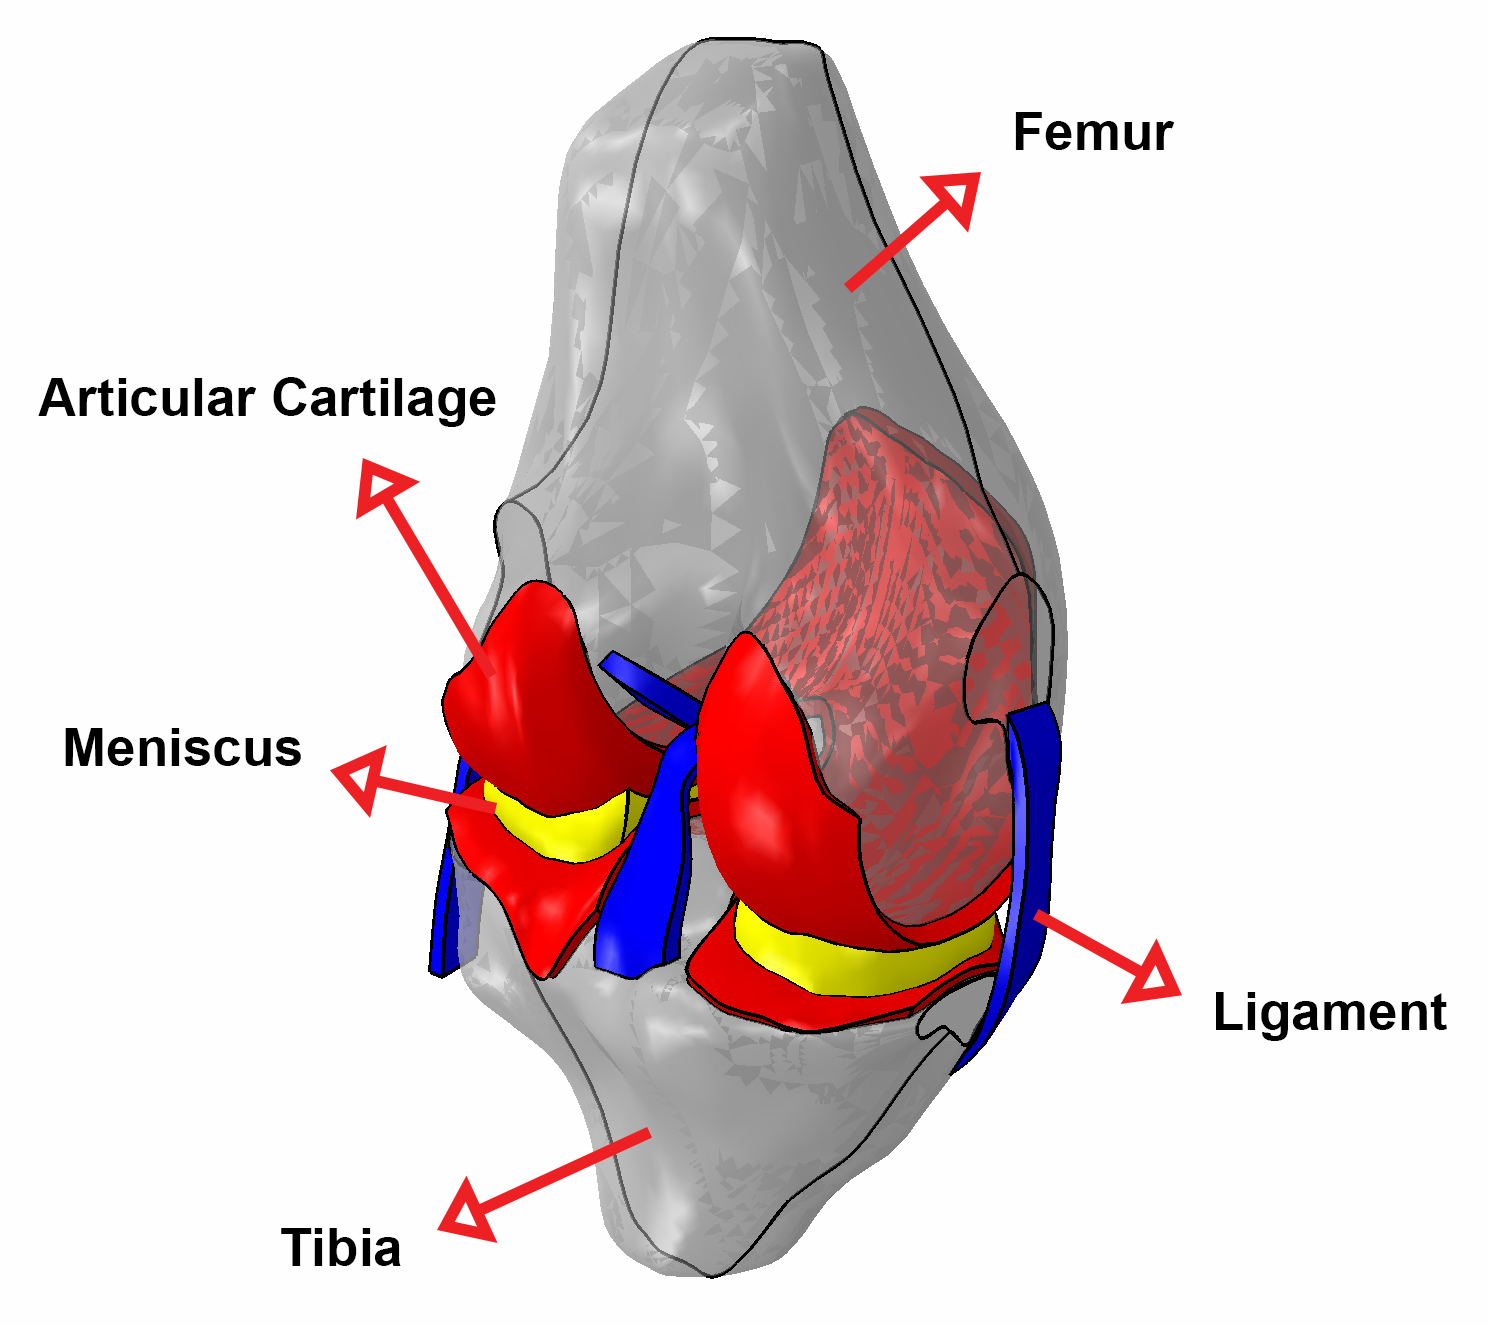
\includegraphics[width=0.6\linewidth]{knee.jpg}
\caption{Main substructures of a tibiofemoral model shown in different colors.
\label{knee}}
\end{figure}

Osteoarthritis is a degenerative ailment that affects cartilage, causing pain, discomfort, and eventual joint malfunction [\cite{lespasio2017}]. Predominantly seen in older individuals, especially women, this condition exerts considerable strain on health organizations due to its socioeconomic implications [\cite{Chen2012,gillian2019}]. Multiple factors, ranging from genetics to lifestyle choices, contribute to its onset [\cite{loeser2016,mobasheri2017,astephen2021}]. To analyze this disease, it is essential to first understand cartilage biomechanics regardless of its damage. Consequently, a significant portion of the research, including this study, has focused on this aspect [\cite{kong2022}].

Similarly to other connective tissues, the functional attributes of \ac{ac} predominantly stem from its extracellular elements, particularly proteoglycans and collagen network [\cite{culav1999,brody2015}]. Given this, biomechanical investigations heavily concentrate on modeling how these elements interplay [\cite{klika2016,ebrahimi2019,sajjadinia2019,lin2021,paz2022}]. This topic is further explored in the following subsection.

\subsection{Tissue-Scale Properties}
\Ac{ac} is an intricate mix of solid and fluid constituents. Around $60-80\%$ of the tissue is water, brought about by the cartilage's osmotic pressure (caused by proteoglycans) and its porous architecture [\cite{cederlund2022}]. This water content does not just ensure smooth lubrication on the cartilage surface but also presents formidable resistance against applied loads on tissue, more than most other microstructural components [\cite{quiroga2017,sajjadinia2019}]. Therefore, it is common to assume a biphasic composition forms \ac{ac} with a fluid phase (water) and an effective solid phase (solid components with other biomechanical parameters like osmotic pressure).

Aggrecans, the most prevalent cartilage proteoglycans, are attached to hyaluronic acid chains, creating aggregates within the collagen network. Owing to its glycosaminoglycan components, these aggregates carry fixed negative charges. This establishes a chemical gradient, causing water attraction through the osmosis mechanism, explaining the presence of water in the tissue [\cite{kiani2002,gomez2020,johnson2021}]. This results in the above-mentioned osmotic pressure which, by counteracting external forces, plays a role in the tissue's load-bearing ability. Furthermore, this internal pressure increases tissue size and stretches the collagen fibrils, resulting in reversible tissue deformation and higher stiffness [\cite{dudhia2005}].

\begin{figure}
\centering
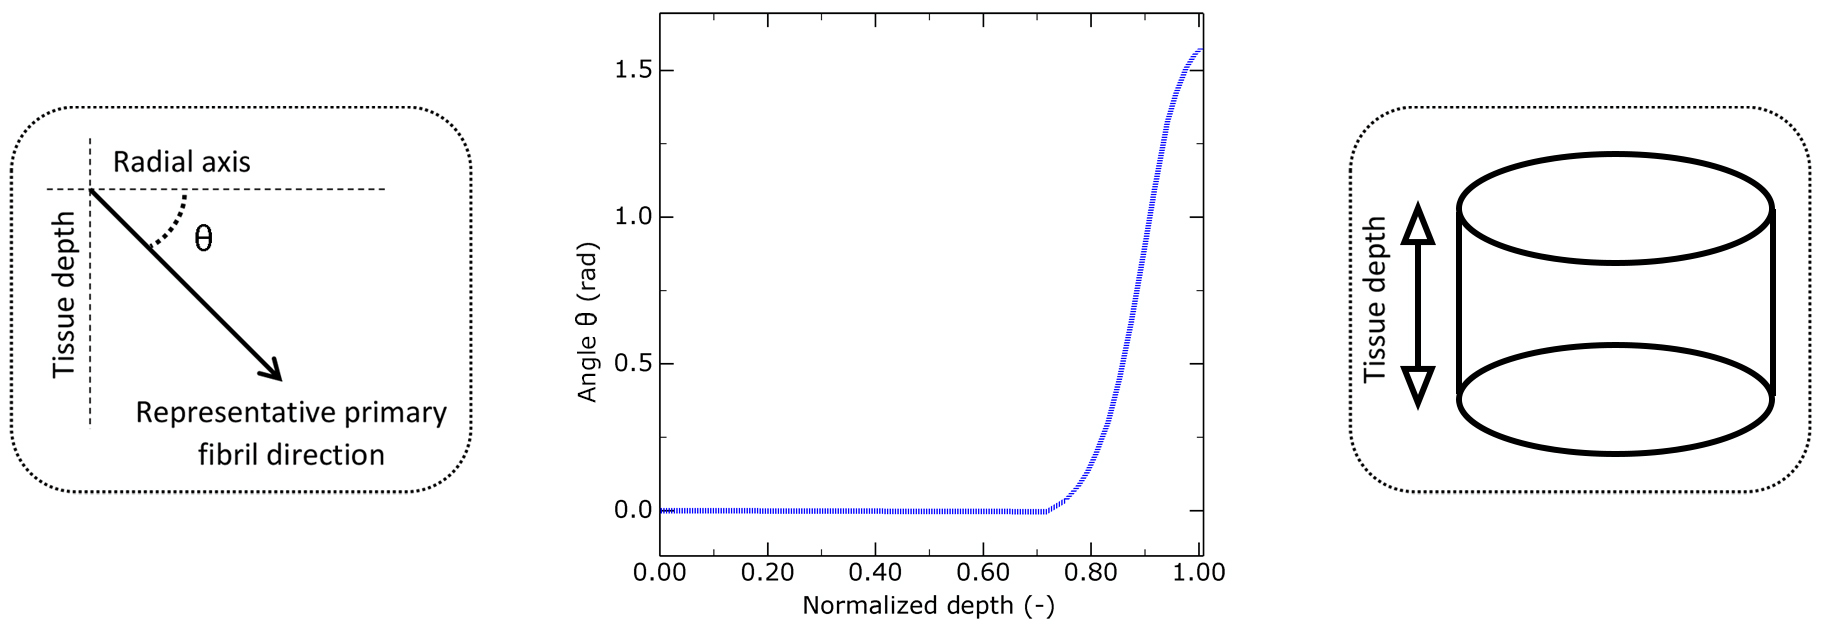
\includegraphics[width=0.9\linewidth]{arcade.jpg}
\caption{In the \emph{in vivo} state of a circular cartilage plug, the angle between the radial axis and one of the primary fibrils is denoted as 
$\uptheta$ for illustration, based on \cite{benninghoff1925} and \cite{wilson2004a} studies.
\label{arcade}}
\end{figure}
%
The extracellular matrix is reinforced by collagen fibrils, which protect \ac{ac} against tensile strains. This is analogous to the reinforcement provided by structural cables, marking it as another significant solid component to consider [\cite{laurent2007,bielajew2020}]. These fibrils can be categorized into primary (anisotropic) and secondary (isotropic) groups [\cite{clark1985,wilson2004a}]. The latter, in healthy tissue, run in all spatial directions, while the former have an arcade-like orientation (Fig.~\ref{arcade}), starting vertically from the deeper \ac{ac} sections and undergoing a mid-course twist to run parallel to the cartilage surface [\cite{wilson2004a}]. These superficial fibrils help protect the surface from shear stresses [\cite{shirazi2008,motavalli2014}]. Therefore, these fibrillar bundles are commonly integrated into mathematical models of cartilage, along with the aforementioned components, as will be discussed in the next section.

\section{Physics-Based Modeling}
%
Note that in the following of this work, we may very occasionally use the same mathematical symbols for different purposes. This is an intentional choice, made to avoid the use of non-standard symbols, and the context can clarify their meanings. Also, note that while ``$:=$'' signifies a definition, ``$:$'' represents the double dot product.

\subsection{Governing Equations}
%
In physics-based modeling of \ac{ac}, inertia and weight are often overlooked due to the tissue's low-density structure [\cite{pearle2005}]. Newton's second law suggests that any force applied to the tissue, or surface traction, will reach equilibrium with other applied forces, leading to cartilage deformation. Below is a simplified representation of the 3D equilibrium equation for this phenomenon:
%
\begin{equation}
    \int_s \mathbf{T} {\rm d}S = \mathbf{0},
\end{equation}
%
where the surface area of the deformed solid material is $S$, and the associated traction on this surface, $\mathbf{T}$, is related to the full Cauchy stress tensor $\boldsymbol{\sigma}_{\rm T}$ as:
%
\begin{equation}\label{eq-traction}
    \mathbf{T} = \boldsymbol{\sigma}_{\rm T} \cdot \textbf{n},
\end{equation}
%
with $\textbf{n}$ being the external normal to the surface. The stress tensor provides a general view of how forces are distributed at each location. Assuming stress as a field parameter and according to the divergence theorem, the flux of the field on a closed surface can be correlated to the field's spatial divergence within the volume $V$. Thus:
%
\begin{equation}
    \int_S \boldsymbol{\sigma}_{\rm T} \cdot \textbf{n} {\rm d}S = \int_V \nabla_\textbf{x} \boldsymbol{\sigma}_{\rm T} {\rm d}V,
\end{equation}
%
where $\nabla_\textbf{x}$ denotes the gradient operator with respect to the position vector after deformation, i.e., $\textbf{x}$. From this, the following differential equation can be deduced without integration [\cite{gerhard-book}]:
%
\begin{equation}\label{eq-strong}
    \nabla_\textbf{x} \boldsymbol{\sigma}_{\rm T} = \textbf{0}.
\end{equation}

For considering the biomechanical role of the fluid phase, the continuity equation can be used. It implies that the rate of change of fluid within the tissue is equal to the amount passing the boundary, based on the premise that \ac{ac} is a water-saturated porous medium:
%
\begin{equation}
    \frac{{\rm d}}{{\rm d}t}\left ( \int_V \rho \phi^{\rm F} {\rm d}V \right ) + \int_S \rho \phi^{\rm F} \textbf{n} \cdot \textbf{v}_{\rm r} {\rm d}S = 0,
\end{equation}
%
where $\textbf{v}_{\rm r}$ is the relative fluid velocity with respect to the solid framework, $\rho$ represents fluid mass density, and $\phi^{\rm F}$ is the local fluid volume fraction. By inserting the volume ratio $J$ in the first term (to account for the solid phase deformation) and applying the divergence theorem to the second term, we get the following partial differential equation:
%
\begin{equation}\label{eq-pde}
    \frac{1}{J}\frac{{\rm d}}{{\rm d}t}\left (J\rho \phi^{\rm F} \right ) + \nabla \cdot \left ( \rho \phi^{\rm F} \textbf{v}_{\rm r} \right ) = 0.
\end{equation}
%
In the next step, the material (constitutive) equations will be defined using finite strain theory, as explained in the following reference [\cite{gerhard-book}].

We assume that $\nabla_\mathbf{X}$ is the gradient operator with respect to the position vector before deformation, $\mathbf{X}$. If $\mathbf{I}$ represents the identity tensor, then the deformation gradient $\mathbf{F}$ is:
%
\begin{equation}
    \mathbf{F} = \nabla_\mathbf{X} \mathbf{u} + \mathbf{I}.
\end{equation}
%
This second-order tensor is a metric of relative deformation, which can be split into the rotation tensor $\mathbf{R}$ and the symmetric tensor that is left stretch tensor $\mathbf{V}$:
%
\begin{equation}
    \mathbf{F} = \mathbf{V} \mathbf{R}. \label{eq1-1}
\end{equation}
%
To eliminate the effects of rigid body rotation on tissue stress and deformation (since inertia effects are ignored), we use the orthogonality of the rotation tensor, i.e., $\mathbf{R}^{\rm T}\mathbf{R} = \mathbf{I}$. Accordingly, the left Cauchy-Green deformation tensor $\mathbf{B}$ is defined to encompass only the stretches, as follows:
%
\begin{equation}
\mathbf{B} = \mathbf{F} \mathbf{F}^{\rm T} = \mathbf{V}^2.
\end{equation}
%
In this way, the volume ratio can also be determined as:
%
\begin{equation}
J = \sqrt{\det \mathbf{B}}.
\end{equation}
%
Next, the logarithmic strain, denoted as $\bm{\epsilon}$, serves as another measure of deformation and is defined by:
%
\begin{equation}
\bm{\epsilon} := \ln \mathbf{B}.
\end{equation}
%
Subsequently, we can use Hook's law, the simplest (linear and isotropic) constitutive model, as follows:
%
\begin{equation}\label{eq-isotropic_elastic}
\bm{\sigma} := \frac{1 + \nu}{E} \left[ \bm{\epsilon} + \frac{\nu}{1 - 2\nu} \left( \mathrm{tr}(\bm{\epsilon}) \mathbf{I} \right) \right].
\end{equation}
%
Here, Young's modulus $E$ and Poisson's ratio $\nu$ are the material constants. A superior alternative is the nearly incompressible neo-Hookean model, which exhibits some nonlinearity during extensive deformations akin to rubber-like materials:
%
\begin{equation}\label{eq-hyperelastic}
\bm{\sigma} :=\frac{2}{J}
\mathbf{F}\frac{\partial\Psi}{\partial\mathbf{C}}\mathbf{F}^{\rm T},
\quad \text{where }
\Psi = C_{10}(\bar{I}_1 - 3) + \frac{1}{D_1}(J - 1)^2.
\end{equation}
%
Here, $\Psi$ represents the empirically defined strain-energy function. The right Cauchy–Green tensor is denoted by \( \mathbf{C} \) and is related by the equation \( \mathbf{C} = \mathbf{F}^{\top} \mathbf{F} \). Moreover, the first invariant of the deviatoric part of \( \mathbf{C} \) is represented as \( \bar{I}_1 \). Notably, this stress definition does not account for the different cartilage phases essential for achieving \ac{hf} results [\cite{gerhard-book}].

To model the interaction between the solid and fluid phases, we employ the well-recognized porous media theory in conjunction with Darcy's law. This law posits that the fluid transition from an area of elevated pressure to one of diminished pressure is determined by the constitutive behavior, such as the dynamic viscosity $\mu$, i.e., the fluid's inherent resistance to flow [\cite{karl1943,fa1979}]:
%
\begin{equation}\label{eq-darcy}
    \phi^F \mathbf{v}_{\rm r} = -\frac{1}{\mu }\mathbf{K} \cdot \nabla_\mathbf{x} P,
\end{equation}
%
where the fluid volume fraction is denoted by $\phi^{\rm F}$ and the permeability tensor $\mathbf{K}$ determines the porous structure's ability to permit fluid flow within the solid matrix. This results in fluid pressure $P$ and effective solid stress $\boldsymbol{\sigma}^{\rm EFF}$ as follows:
%
\begin{equation}\label{eq-stress}
    \boldsymbol{\sigma} :=  \boldsymbol{\sigma}^{\rm EFF} - P\mathbf{I}.
\end{equation}
%
The constrained mixture theory~[\cite{klisch1999}] is frequently adopted to account for the contributions of different phases to the effective stress in AC. According to this theory, non-fluid segments are bound to each other, leading them to exhibit similar deformation. This is expressed as:
%
\begin{equation}\label{eq-cartilage_solid}
    \boldsymbol{\sigma}^{\rm{EFF}} :=  \boldsymbol{\sigma}^{\rm{COL}} + \boldsymbol{\sigma}^{\rm{MAT}} - \boldsymbol{\sigma}^{\rm{GAG}}.
\end{equation}
%
Within this framework, the annotations ${\rm COL}$, ${\rm MAT}$, and ${\rm GAG}$ denote the stress contributions from the collagen network, the non-fibrillar solid matrix, and the osmotic pressure, respectively~[\cite{mow1980,wilson2005,sajjadinia2019}].

Regarding the osmotic pressure, it can be approximated by the electrostatic forces of glycosaminoglycans. This force is also strictly associated with solid matrix deformation [\cite{ateshian2004}]. Making this assumption simplifies the expression to an exponential form with material constants \(\alpha_1\) and \(\alpha_2\) [\cite{ateshian2004,buschmann1995,stender2013}]:
%
\begin{equation}\label{eq-osmotic}
    \boldsymbol{\sigma}^{\text{GAG}} = \alpha_1 J^{-\alpha_2} \mathbf{I}.
\end{equation}
%
As to the collagen fibrils, a nonlinear relationship between loads and strains is evident through experimentation [\cite{charlebois2004}]. Focusing on a specific fibrillar bundle $I$, this relationship can be represented as $(E_1 + E_2 \epsilon^I) \epsilon^I$, with $E_1$ and $E_2$ highlighting the nonlinearity extent. Then,
%
\begin{equation}
    \epsilon^I = \log (\lambda^I).
\end{equation}
%
Here, the fibrillar stretch is represented by $\lambda^I$, which is related to the total deformation by
%
\begin{equation}\label{eq:phi}
    \lambda^I = \sqrt{\mathbf{n}^I \cdot \mathbf{B} \cdot\mathbf{n}^I},
\end{equation}
where, $\mathbf{n}^I$ is the new direction of the fibril bundle $I$ after deformation, which is correlated with the initial direction vector $\mathbf{N}^I$ via 
%
\begin{equation}\label{eq:n}
\mathbf{n}^I = \frac{\mathbf{F} \cdot \mathbf{N}^I}{\left \| \mathbf{F} \cdot\mathbf{N}^I \right \|_{2}},
\end{equation}
%
where $\left \| \bullet \right \|_{2}$ denotes the $l^2$ norm of $\bullet$.  Furthermore, to account for surface area variations, the aforementioned constitutive equation of fibril $I$ can be multiplied with $\lambda^I/J$, the inverse of the surface area of the fibril bundle, yielding
%
\begin{equation}
    \sigma^I = \phi^{\rm S}_0 \rho_{\rm C}^I \frac{\lambda^I}{J}(E_1 + E_2 \epsilon^I) \epsilon^I \quad \text{if } \epsilon^I > 0,
\end{equation}
%
where, $\rho_{\rm C}^I$ represents the volume fraction of pertinent fibrils and $\phi^{\rm S}_0$ indicates the solid's initial volume fraction. The volume fractions are inserted in the equation to encompass the contribution of each phase based on mixture theory. Considering the compressibility of the porous solid structure of cartilage, these values are updated by the continuity equation, as follows
%
\begin{equation}
    \label{continuity}
    \varphi = \frac{\varphi_0}{J} 
    \qquad 
    \varphi \in \left \{\phi^{\rm S}, \: \rho^{\rm COL} \right \}.
\end{equation}
%
Now, the total stress in the collagen fibrils at all directions, expressed as $\boldsymbol{\sigma}^{\rm COL}$ can be determined by [\cite{wilson2004a}]:
%
\begin{equation}\label{eq-fibril_stress}
    \boldsymbol{\sigma}^{\rm COL} = \sum_{I=1}^9 \sigma^I \mathbf{n}^I \otimes \mathbf{n}^I,
\end{equation}
%
where $\otimes$ represents the dyadic product.

Finally, the other parts of the solid material can be modeled by nonlinear isotropic elastic models. One such common model is the neo-Hookean equation, grounded in rubber-like material thermodynamics [\cite{kim2012}]. This equation is adjusted to reflect the volume fractions of the material components [\cite{wilson2007,sajjadinia2019}]:
%
\begin{equation}\label{eq-non_fibrillar}
    \boldsymbol{\sigma}^{\rm MAT} = 
    \phi^{\rm S}_0 G_m \frac{1 - \rho_0^{\rm COL}}{J} \left[\frac{\ln{J}}{2} 
    \left( \frac{1}{3} + \frac{J + \phi^{\rm S}_0}{J - \phi^{\rm S}_0} - \frac{\phi^{\rm S}_0 J\ln{J}}{( J - \phi^{\rm S}_0)^2} \right) \mathbf{I} 
    + (\mathbf{B} - J^{2/3}\mathbf{I}) \right].
\end{equation}
%
Here, \( G_m \) is a material constant. Hence, the stress in the components of this \ac{hf} multi-physics model correlates with the deformation in the tissue.

The multiphasic model can be further simplified either by ignoring the contributions of some of its components or by using an alternative monophasic (elastic) model. An additional possible assumption in monophasic models is to incorporate a level of viscosity to model the time-dependent response (without including the fluid phase that makes biphasic models time-dependent). To exemplify a viscoelastic model, we first denote the deviatoric (DEV) and hydrostatic parts of a symmetrical second-order tensor \textbf{A} with superscripts \textit{D} and \textit{H}, respectively. Accordingly, we have [\cite{backus1970}]
%
\begin{equation}
    \text{DEV} (\textbf{A}) = \textbf{A} - \textbf{A}^{H}, \quad \text{where } \textbf{A}^{H} = \frac{1}{3}\text{tr}(\textbf{A})\mathbf{I}.
\end{equation}
%
Defining the Kirchhoff stress $\boldsymbol{\tau}=J\boldsymbol{\sigma}$, its instantaneous value (without viscosity) is denoted by the subscript 0. Then, a simplified viscoelastic model is formulated as:
%
\begin{align}\label{eq-visco}
    \boldsymbol{\tau} &= \boldsymbol{\tau}_{0} - \text{DEV}\left[ \frac{\mathcal{G}}{\mathcal{T}} \int_{0}^{t} \mathbf{\bar{F}}_{t}^{-1}(t-s) \cdot \text{DEV}(\boldsymbol{\tau}_{0}(t-s)) \cdot \mathbf{\bar{F}}_{t}^{-T}(t-s) e^{-s/\mathcal{T}} \, ds\right] \\
    &-  \frac{\mathcal{K}}{\mathcal{T}} \int_{0}^{t} \boldsymbol{\tau}_{0}^{H}(t-s) e^{-s/\mathcal{T}} \, ds.
\end{align}
%
Here, $\mathbf{\bar{F}}_{t}^{-1}(t-s)=\mathbf{\bar{F}}(t)\cdot\mathbf{\bar{F}}^{-1}(t-s)$ and its transposed are used as a transformation operator to shift the stress tensor to the current configuration (as it can be rotated for the deviatoric part), where $\mathbf{\bar{F}} = J^{-1/3}\mathbf{F}$ is the distortion gradient (disregarding the volume change since $\det \mathbf{\bar{F}}=1$). Also, $\mathcal{G}$ and $\mathcal{K}$ are material constants controlling the time-dependent shear and bulk moduli, respectively, while $\mathcal{T}$ is another constitutive constant controlling the tissue relaxation time until equilibrium is reached [\cite{fazekas2018,abaqus,simo1987}].



\subsection{Implicit Finite Element Analysis}
%
The algorithms behind \ac{fe} analysis typically make use of the weak formulation of differential equations. For this reason, the virtual work principle [\cite{antman1979}] can be applied to the eq.~(\ref{eq-strong}), yielding to
%
\begin{equation}\label{eq-weak-alt}
    \int_V \boldsymbol{\sigma}_{\mathrm{T}} \nabla_\mathbf{x} \cdot \delta \mathbf{u} \, \mathrm{d}V = 0,
\end{equation}
%
with $\delta \mathbf{u}$ signifying the virtual displacement vector contributing to the virtual work. This way, the strong form, eq.~\ref{eq-strong}, is transformed into a simpler equation with scalar output due to the existence of the integrals and dot product. Next, by applying integration by parts, the divergence theorem, and leveraging eq.~\ref{eq-traction}, boundary, and volumetric parts are distinguished, as follows [\cite{gerhard-book,belytschko2014}]:
%
\begin{equation}
    \int_V \delta \mathbf{u} \nabla_\mathbf{x} \boldsymbol{\sigma}_{\mathrm{T}} \, \mathrm{d}V - \int_S \mathbf{T} \delta \mathbf{u} \, \mathrm{d}S = 0.
\label{eq-alt-dode}
\end{equation}
%
In case the fluid phase is also modeled, we first discretize the time derivatives using finite differences, particularly through the backward Euler approach. For instance, applying this to a function $y$, in this case the first term of eq.~\ref{eq-pde}, results in
%
\begin{equation}
    \frac{\mathrm{d}y}{\mathrm{d}t} \bigg|_{t+\Delta t} \approx \frac{y_{t+\Delta t} - y_t}{\Delta t}.
\end{equation}
%
After finding the derivative and then finding the weak form with a method similar to the weak form derivation of the equilibrium equation, a weak formulation for this equation is also obtained using
%
\begin{eqnarray}
    & & \int_V \left( \left[ \delta P \right]_{t+\Delta t} \left( \left[ J \rho \phi^{\rm F} \right]_{t+\Delta t} - \left[ J \rho \phi^{\rm F} \right]_{t} \right) - \Delta t \left[ \rho \phi^{\rm F} \nabla_{\mathbf{x}} \delta P \cdot \mathbf{v}_{\rm r} \right]_{t+\Delta t} \right) \, \mathrm{d}V \nonumber \\
    & & + \Delta t \int_S \left[ \delta P \rho \phi^{\rm F} \mathbf{n} \cdot \mathbf{v}_{\rm r} \right]_{t+\Delta t} \, \mathrm{d}S = 0,\label{eq-fluid}
\end{eqnarray}
%
where $\delta P$ indicates the virtual fluid pressure. Combining this with eq.~\ref{eq-darcy} gives
%
\begin{eqnarray}\label{eq-fluid-2}
    & & \int_V \left( \left[ \delta P \right]_{t+\Delta t} \left( \left[ J \rho \phi^{\rm F} \right]_{t+\Delta t} - \left[ J \rho \phi^{\rm F} \right]_{t} \right) - \Delta t \left[ \rho \phi^{\rm F} \nabla_{\mathbf{x}} \delta P \cdot \mathbf{v}_{\rm r} \right]_{t+\Delta t} \right) \, \mathrm{d}V \nonumber \\
    & & - \Delta t \int_S \left[ \delta P \frac{\rho}{\mu } \mathbf{n} \cdot \mathbf{K} \cdot \nabla_\mathbf{x} P \right]_{t+\Delta t} \, \mathrm{d}S = 0.
\end{eqnarray}
%
This equation, together with eq.~\ref{eq-alt-dode} with one of the solid constitutive equations applied, defines the possible weak formulation in which the integrals can be calculated numerically after discretizing the physics domain into smaller elements, called \ac{fe}s.

For clarification of the spatial discretization in \ac{fe} analysis, a nonlinear 1D function, \( f(x) \), is exemplified by its approximation after discretization, \( \bar{f}(x) \):
%
\begin{equation}\label{eq-alt-shape}
    \bar{f}(x) = \sum_{i=1}^{n} \mathcal{N}^{i}(x) f(x_i),
\end{equation}
%
where the spatial space is divided into 1D \ac{fe}s with nodal inputs \( x_i \) associated with outcomes \( f(x_i) \) over the domain \( [x_{i-1}, x_i] \) of element $i$. The defined shape functions of the element, \( \mathcal{N}^i(x) \), are then expressed on two nodes, as follows:
%
\begin{equation}
    \mathcal{N}_1^{i}(x) = \frac{x - x_{i-1}}{x_i - x_{i-1}} 
    \quad \text{and} \quad 
    \mathcal{N}_2^{i}(x) = \frac{x_i - x}{x_i - x_{i-1}}.
\end{equation}
%
These shape or interpolation functions represent \( f(x) \) as a sequence of interconnected simpler functions at the nodal points. In practice, the interpolation can be of higher order and dimensions, allowing more accurate numerical integrations, as illustrated in Fig.~\ref{fea}.
%
\begin{figure}
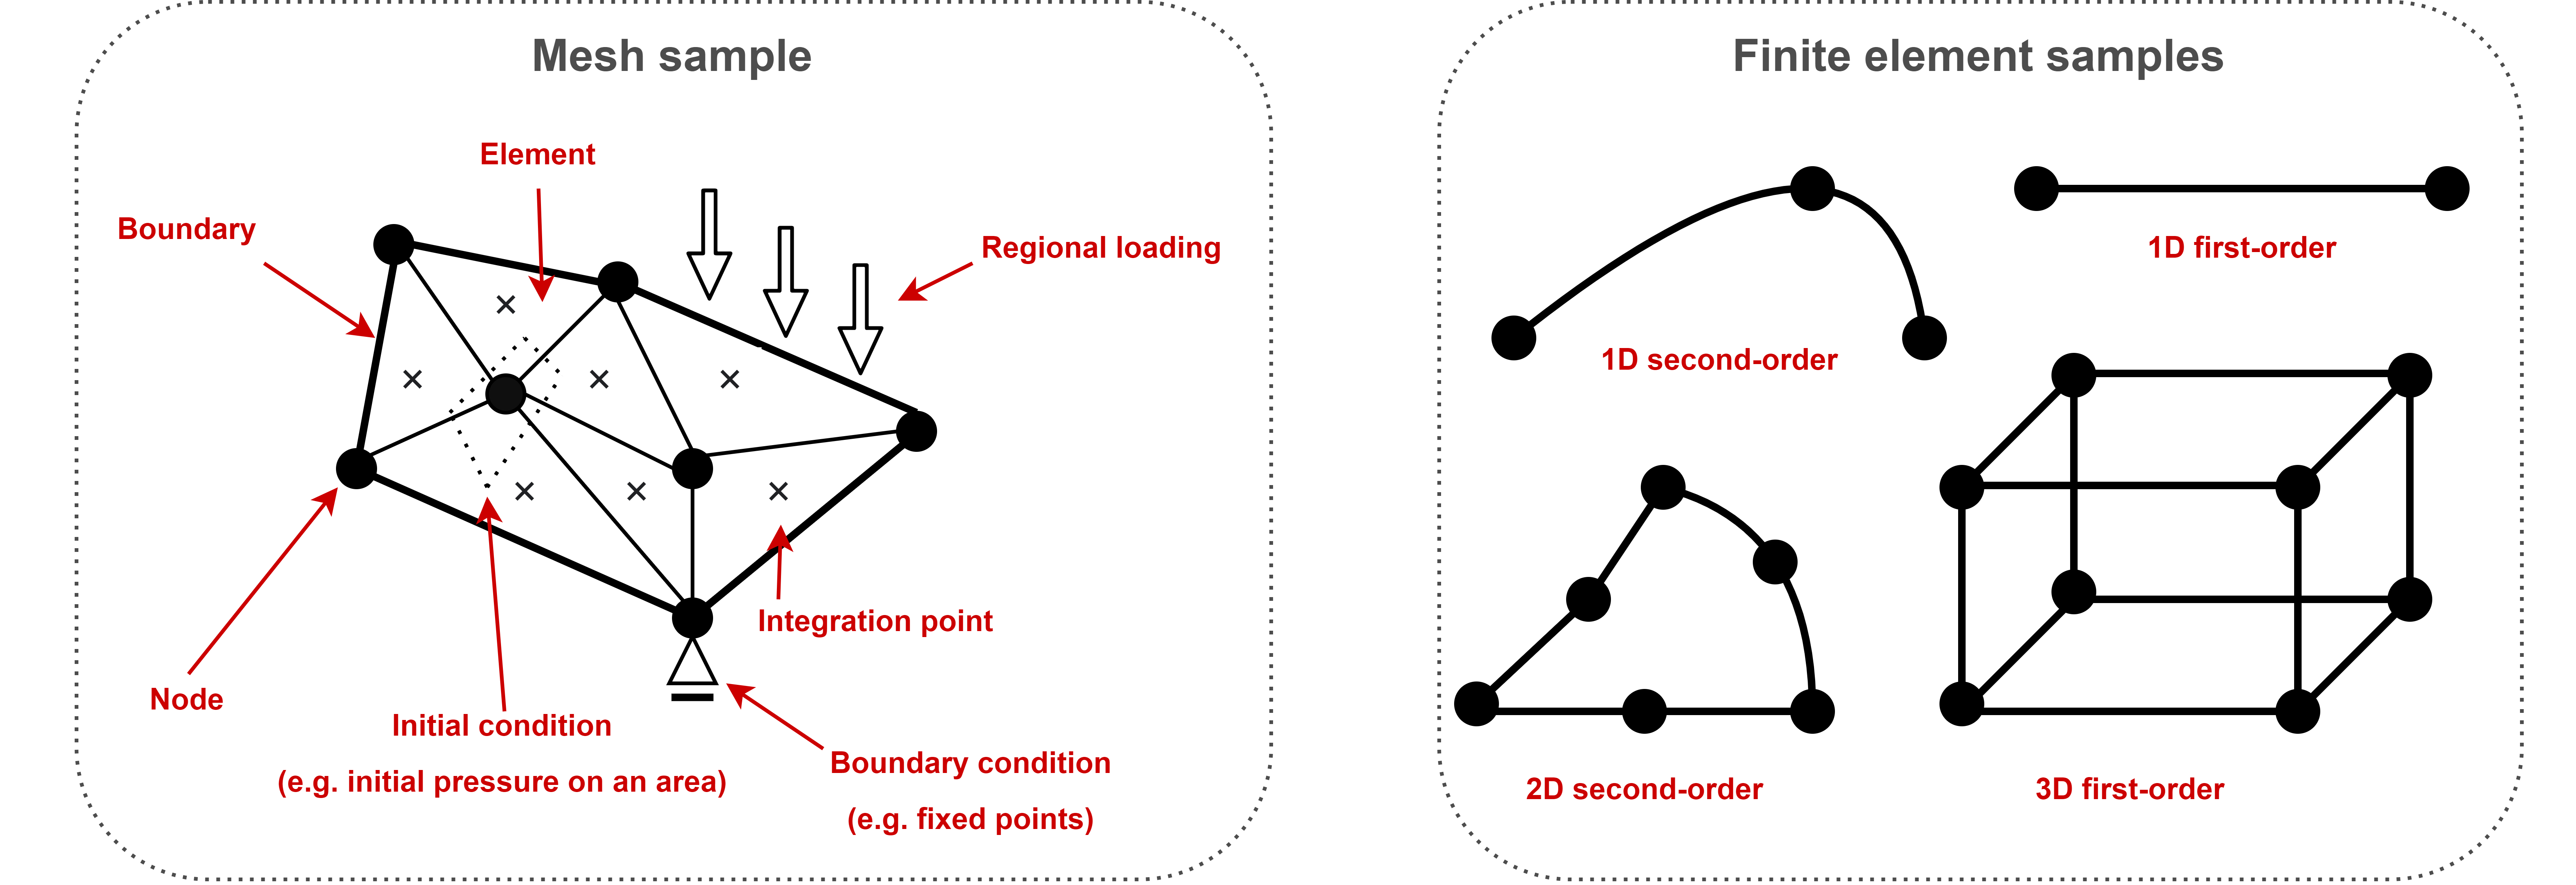
\includegraphics[width=1\linewidth]{fea.png}
\caption{Examples of \acp{fe} and mesh entities: typically, the geometric domain is discretized into \acp{fe}, and the boundary conditions are applied to the nodes. In this manner, integrals are computed at integration points and are then usually extrapolated to the nodes. The choice of element definition depends on dimensionality and physical characteristics, such as geometric complexity.}
\label{fea}
\end{figure}

Extending the concept of 1D \acp{fe} to 3D space of this multi-physics equation, shape functions, \( \mathcal{N}^P \) and \( \mathcal{N}^\mathbf{u} \), are introduced similarly for spatial discretization of \( P \) and \( \mathbf{u} \) (along with their virtual variations). Inserting them into eqs.~\ref{eq-fluid-2} and \ref{eq-alt-dode}, we get

%
\begin{equation}
    \mathcal{F} =
    \begin{bmatrix}
        \left[\int_V \mathcal{N}^\textbf{u} \nabla_\textbf{x} \boldsymbol{\sigma} \, {\mathrm d}V - \int_S \textbf{T} \mathcal{N}^\textbf{u} \, {\mathrm d}S\right]_{t+\Delta t} \\
        \begin{aligned}
            &\int_V \left ( \mathcal{N}^p_{t+\Delta t} \left( \left[ J \rho \phi^F \right]_{t+\Delta t} - \left[ J \rho \phi^F \right]_{t} \right) - \Delta t \left[ \rho \phi^F \nabla_{\mathbf{x}} \mathcal{N}^p \cdot \mathbf{v}_{\rm r} \right]_{t+\Delta t} \right) \, {\mathrm d}V \\
            &\hookrightarrow + \Delta t \int_S \left[ \mathcal{N}^p \frac{\rho}{\mu } \mathbf{n} \cdot \mathbf{K} \cdot \nabla_\mathbf{x} \mathcal{N}^p \bar{P} \right]_{t+\Delta t} \, {\mathrm d}S
        \end{aligned}
    \end{bmatrix}
    = \textbf{0}.
    \label{eq:alt-deq-matrix}
\end{equation}
%
Since both of the shape functions are geometrical functions, their gradients can be determined. Therefore, the governing equations are fully discretized, and all derivatives are approximated. The final form of this equation depends on the exact formulation of the shape functions, the selected constitutive equations, the numerical integration method, and the dimensionality of the problem. Depending on the fidelity, the final form can be different, for instance, when viscosity is used instead of the fluid pressure, or when contact equations are also added [\cite{pore2021,orava2022,orozco2022,oleg2023}]. Therefore, eq.~\ref{eq:alt-deq-matrix} is merely an illustrative example, and as we used \cite{abaqus} here, interested readers might refer to its documentation for more specific equations.

This approach is termed implicit \ac{fe} analysis, as it yields equations connecting unknown parameters at $t + \Delta t$ with known values at time $t$ after discretization. By the way, it remains a set of nonlinear equations that first need to be linearized and then solved, for example, by Newton's method [\cite{almeida1997,belytschko2014}]. In this regard, the system's variables, in this case, $\left\{ u_1, u_2, u_3, P \right\}$, are denoted by $\mathfrak{U}$. In the 3D Cartesian system, $u_1, u_2$, and $u_3$ are the $\mathbf{u}$ components. To apply Newton's method for linearizing eq.~\ref{eq:alt-deq-matrix}, represented by $\mathcal{F}$, the Jacobian matrix $\mathfrak{J}^{(i)}$ is used during each iteration step $i$. This matrix is formulated as
%
\begin{equation}
    \label{eq:j}
    \mathfrak{J}^{(i)} := \begin{bmatrix}
        \frac{\partial \mathcal{F}^{(i)}_1}{\partial u^{(i)}_1} & \cdots & \frac{\partial \mathcal{F}^{(i)}_1}{\partial P^{(i)}}\\
        \frac{\partial \mathcal{F}^{(i)}_2}{\partial u^{(i)}_1} & \cdots & \frac{\partial \mathcal{F}^{(i)}_2}{\partial P^{(i)}}
    \end{bmatrix},
\end{equation}
%
with
%
\begin{equation}
    \mathcal{F}^{(i)} := \mathcal{F}\Big|_{\substack{\mathfrak{U}^t=\mathfrak{U}^{(i-1)}, \: \mathfrak{U}^{t+\Delta t}=\mathfrak{U}^{(i)}}}.
\end{equation}
%
Let $\mathfrak{U}^{(0)}$ be the known value of $\mathfrak{U}$ determined at the start of the increment, using $\mathfrak{U}^{(1)}$ as the initial guess, the nonlinear equations are linearized sequentially as:
%
\begin{equation}\label{eq-fea_opt}
    \mathcal{F}^{(i+1)} := \mathcal{F}^{(i)} + \left ( \mathfrak{U}^{(i+1)} - \mathfrak{U}^{(i)} \right ) \cdot \mathfrak{J}^{(i)}.
\end{equation}
%
These linear equations can then be solved using any standard linear algebra techniques to determine $\mathfrak{U}^{(i+1)}$. Convergence is confirmed when $\mathcal{F}^{(i+1)}$ approaches zero, indicating that the unknowns are well-approximated [\cite{belytschko2014}].

A user of Abaqus can define numerical problems, such as boundary conditions, geometry, constitutive behavior, element formulation, and more. The software implements eq.~\ref{eq-fea_opt} for the specified problem automatically, and its integration with Python scripts, simplifies numerical implementation. However, implementing a multiphasic model is an exception. Although Abaqus can approximate biphasic behavior using the soil consolidation theory [\cite{verruijt1984}], Fortran subroutines are necessary for implementing multiphasic equations. In these subroutines, eq.~\ref{eq-cartilage_solid} is directly coded along with its contribution to the Jacobian matrix (eq.~\ref{eq:j}). This can be approximated using a generic finite difference algorithm [\cite{miehe1996}]. Interested readers might refer to previous tutorials [\cite{nolan2022,fehervary2020}] for more details.

Such numeral methods, while could be expensive, still might systematically generate training data for possibly efficient surrogate modeling. These \ac{ml}-based algorithms are commonly implemented using deep learning, as explained in the following.

\section{Data-Driven Modeling}
\subsection{Deep Learning}

In supervised machine learning, the central task involves designing a model function $f$, mapping each element in a set of input data $\mathcal{X}$ to a corresponding element in an output set $\mathcal{Y}$. This relationship is mathematically expressed as $f: \mathcal{X} \longrightarrow \mathcal{Y}.$ The elements in $\mathcal{Y}$, also known as labels, are derived from either human or automated supervision, and are used to develop and assess the model. These labels, in conjunction with input data, are characterized by multidimensional features. For instance, if the values of boundary conditions in a simulation can be seen as the input features, the labels would be the observed or calculated deformation in the tissue.

Deep learning algorithms, like many of the other supervised machine learning methods, seek the most effective function $f$ using a group of labeled data $\mathcal{Z}\subset \mathcal{X} \times \mathcal{Y}$ and applying an optimization algorithm. This is achieved through minimizing errors, quantified by a loss function $\mathcal{L}: \mathcal{M} \left ( \mathcal{X},\mathcal{Y} \right ) \times \mathcal{Z} \longrightarrow \mathbb{R},$ where $\mathcal{M}$ denotes the set of all potential learnable functions, which can have various hypothetical definitions like different artificial neural networks [\cite{abiodun2019}].

A simple network is the multi-layer \ac{ffnn}, which links a sequence of input features through dense (fully connected) layers to subsequent layers until the final output layer is reached [\cite{rumelhart1986}]. For an FFNN model $\Psi \in \mathcal{M}\left ( \mathcal{X},\mathcal{Y} \right )$ with $L$ layers, the function can be expressed as:
%
\begin{equation}\label{eq-ffnn}
\Psi (x; \cdot, \Theta )= \psi^{(L)} \left( \psi^{(L-1)} \left(\cdots \left(\psi^{(1)} \left( \psi^{(0)} \left(x \right ) \right ) \right )\right )\right ).
\end{equation}
%
In this model, $\psi^{(i)}$ represents the transformation through layer $i$, with $0$ being the input layer, and $\Theta$ includes the set of trainable parameters to be determined by the optimization algorithm. The simplest form of $\psi^{(i)}$ for regression problems is:
%
\begin{equation}\label{eq-layer}
    \psi^{(i)}(x) = \begin{cases}
        W^{(L)}\psi^{(L-1)}(x) + b^{(L)}, & \text{if } i = L, \\ 
        a \left( W^{(i)}\psi^{(i-1)}(x) + b^{(i)} \right), & \text{otherwise},
    \end{cases}
\end{equation}
%
where $W$ and $b$ are the vectors of weight and bias parameters, and $a(\cdot)$ is the activation function, which introduces nonlinearity to capture complex nonlinear patterns [\cite{berner2022}]. Accordingly, a neuron, which is the most basic computational unit, is each member of $\psi^{(i)}$.

A common activation function, used in eq.~\ref{eq-layer}, is the rectified linear unit (ReLU) [\cite{fukushima1980,nair2010}], defined as:
%
\begin{equation}
\text{ReLU}(x) = \max(0, x).
\end{equation}
%
This piecewise linear function only outputs the positive input signal that mimics the threshold-based firing in biological neurons. Due to the simplicity of this function, it has many optimized implementations, and therefore it is highly used.  However, it can encounter the "dying ReLU" issue during optimization, where the neurons might become too inactive. A frequently used alternative is the exponential linear unit (ELU) which defines a small exponential function for the negative signal, as follows :
%
\begin{equation}
 \text{ELU}(x;\lambda^{\text{ELU}}) = 
\begin{cases} 
x & \text{if } x > 0, \\
\lambda^{\text{ELU}} (e^x - 1) & \text{if } x \leq 0,
\end{cases}
\end{equation}
%
where $\lambda^{\text{ELU}}$ is a hyperparameter, meaning it is a parameter that cannot be learned and must be specified by the user to define the network architecture. During the training process, an initial guess is made for the learnable parameters ($\Theta$), which are then iteratively adjusted by the optimizer based on the parameter gradient. While it is possible to adjust hyperparameters using another optimizer, this approach, known as hyperparameter search or tuning, can be overly time-consuming. Therefore, especially in the context of this study, hyperparameters are usually set by the user through trial and error, especially by considering commonly applied settings.

The input during training consists of batches of concatenated samples. A large batch size can accelerate training by processing larger chunks of data, while a smaller batch size introduces noise into the training process. This noise can help the optimizer escape suboptimal local minima. Additionally, deep neural networks often encounter the issue of vanishing or exploding gradients, stemming from inconsistent scaling of network signal values. A common modification to eq.~\ref{eq-ffnn} involves using normalization layers either after or before each hidden layer, typically applied on either the batch or feature dimension. Although the input layer is usually normalized for the same reason, the output layer is sometimes normalized as well, especially if the features are of different scales. This approach enables more stable training and convergence [\cite{ioffe2015, bjorck2018, jingjing2019, gao2020, singh2022}].

In addition to normalization, the method used for parameter initialization also determines the speed of convergence. These methods sample parameters for each layer in proportion to the number of input or output signals so that each layer with a higher number of signals has a smaller variance range. Thus, during training initialization, the network may maintain a consistent layer-wise variance of activations and gradients across layers. The Xavier initialization technique [\cite{glorot2010}] considers both input and output signals, whereas the He initialization [\cite{he2015}] assumes the number of output signals to be the same as the inputs, which might be more appropriate with certain activation functions [\cite{mlbook}].

Alternatively, the LeCun initialization [\cite{lecun2012}] only considers the input signals, which may be more suitable for the scaled ELU (SELU) activation function [\cite{klambauer2017, mlbook}]. This function is a scaled version of the ELU function that empirically ensures self-normalization, thus potentially obviating the need for normalization layers. It is defined as follows:
%
\begin{equation}
 \text{SELU}(x) \approx 1.0507 \begin{cases} 
x & \text{if } x > 0, \\
1.6733 ( e^x - 1) & \text{if } x \leq 0 .
\end{cases}
\end{equation}

Regardless of the selected training settings and network architecture, once the parameters are initialized, optimizers adjust them by:
%
\begin{equation}\label{eq-optimization}
\theta_{t+1} = \theta_t - \alpha U_t,
\end{equation}
%
where \(\alpha\) is the learning rate hyperparameter and \(U_t\) is the update function. In the context of deep learning, where high-order optimizers could be ill-conditioned due to the noise in each mini-batch of labeled data, Adam, a popular and efficient first-order optimizer, is used. This optimizer is an extension and combination of previous first-order optimization methods [\cite{kiefer1952, polyak1964, nesterov1983, duchi2011, hinton2012}], defined by:
%
\begin{equation}\label{eq-update}
U_t = \frac{\hat{m}_t}{\sqrt{\hat{v}_t} + \epsilon},
\end{equation}
%
with \(\epsilon\) being a small constant to prevent zero-division. Also, \(\hat{m}_t\) and \(\hat{v}_t\) are respectively the modified first and second moments, defined by:
%
\begin{equation}\label{eq-momont1}
\hat{m}_t = \frac{m_t}{1-\beta_1^t},
\end{equation}
%
\begin{equation}\label{eq-momont2}
\hat{v}_t = \frac{v_t}{1-\beta_2^t},
\end{equation}
%
where \(\beta_1\) and \(\beta_2\) are typically hyperparameters close to one. \(m\) and \(v\) are respectively the mean and variance estimates, updated by:
%
\begin{equation}\label{eq-momont1update}
{m}_t = \beta_1{m}_{t-1} + (1-\beta_1)\nabla_{\Theta} \mathcal{L}(\Theta_t)
\end{equation}
%
\begin{equation}\label{eq-momont2update}
{v}_t = \beta_2 {v}_{t-1} + (1-\beta_2)\left(\nabla_{\Theta} \mathcal{L}(\Theta_t)\right)^2.
\end{equation}
%
Conceptually, since these metrics are initially zeroed, they are biased toward small values in the early iterations, and therefore their values are augmented by eqs.~\ref{eq-momont1} \& \ref{eq-momont2}. The hyperparameters in eqs.~\ref{eq-momont1update} \& \ref{eq-momont2update} help in smoothing out the updates to dampen oscillations. These accumulations of gradient and its standard deviation are then applied into eq.~\ref{eq-update} so that it adaptively scales down the gradients with huge variances to avoid overshooting the global minimum.

To implement eq.~\ref{eq-optimization}, a loss function should be selected to measure prediction error. Since our deep learning problems here are regression tasks, where even the outliers (like irregular numerical noises) are significant, we used the \(l_2\) loss, known as the \ac{mse}, which is basically the Euclidean distance between the prediction vector and target vector. This differentiable function can now be differentiated, and then, using the chain rule of calculus, it can be related to the gradient of each parameter, i.e., \(\nabla_{\Theta} \mathcal{L}(\Theta_t)\). This process is known as the backpropagation algorithm [\cite{rumelhart1986}], where the gradient is calculated in a backward manner, from the output to the input layers, typically using an automatic differentiation algorithm; see the [\cite{baydin2018}] study for further details.

One of the key aspects of training involves the training loop, where a batch of input data is fed into the model, and the parameters are updated based on the loss function and optimization algorithm. This loop repeats until all data in the training set has been processed, marking the completion of an epoch. Metrics such as MSE are used to assess model performance on different data splits (training, validation, and testing sets), which helps in evaluating the model's generalizability to unseen data. The distinction between in-distribution and out-of-distribution testing errors is made based on the similarity of the testing set to the training set. Additionally, to prevent overfitting, an early stopping mechanism is often employed where the training process is halted if the validation error starts increasing. This ensures that the model retains its generalization ability and does not become overly complex for the given data [\cite{mlbook}].

In practical terms, deep learning models especially for regression tasks, such as those described in this study, are typically implemented using high-level libraries like Keras [\cite{chollet2015}] or Sonnet [\cite{reynolds2017}], together with TensorFlow [\cite{abadi2015}] and other Python tools [\cite{hunter2007,pedregosa2011,kluyver2016,harris2020,virtanen2020}]. These libraries provide a rich set of tools, including built-in network elements, data handling utilities, and automatic implementation of training optimizers and backpropagation. This simplifies the process of setting up and training a model, as most of the complex underlying mechanisms are abstractly handled by the libraries. The user's primary task is to define the network architecture, after which these tools take care of the iterative training process. Also, although these tools offer utilities to help manage overfitting, we chose simplified models for faster training in this study and did not use them. Our main challenge is indeed to prevent underfitting, which can lead to suboptimal performance.

On the other hand, deep learning can also be applied in an unsupervised, or more precisely, self-supervised manner, where the input and output data are the same. These so-called \acp{ae} are designed to learn typically reduced representations (encodings), which are then reconstructed by a decoder and implemented using regular \ac{ffnn}. The primary use case is for dimensionality reduction. However, a notable variation is the denoising \ac{ae}, which involves adding artificial noise to the data in a preprocessing step (often referred to as \ac{da} since it generates new samples). The DAE then learns to remove this noise [\cite{hinton2006,vincent2008}].

Another deep learning model used in this study is the message-passing \acp{gnn}, which allow for permutation invariance, meaning that the input data can be fed in different orders. In such \acp{gnn}, the focus is on local behavior, particularly on a graph node and its neighbors. This updates the nodal representations as follows:
%
\begin{equation}
\label{eq:gnn}
\mathfrak{v}'_n = \text{FFNN} \left(\sum_{i \in \Gamma(n)}\mathfrak{v}_i, \mathfrak{v}_n\right),
\end{equation}
%
where $\mathfrak{v}'_n$ is the updated nodal feature. The effectiveness of the model can be further enhanced by incorporating edge features and updating them with another \ac{ffnn} [\cite{cai2018,zhou2020,wu2021}]. The main application here is in scenarios where geometrical generalizability is critical. This is achieved by first learning local behavior and then generalizing to other geometries.

In summary, the selection of a DL method depends largely on the objectives at hand, with a focus on employing such learnable \ac{ai} systems instead of relying on predefined physical models. This approach, particularly in the current era dominated by Python and its extensive libraries, becomes increasingly feasible given the availability of sufficient data and computational resources.

\subsection{Surrogate Modeling}
%
Surrogate methodologies offer a synergy of data-driven strategies and computational analytics, providing efficient simulators widely applied in diverse fields such as healthcare [\cite{holzapfel2021,shim2020,liang2018b}] and engineering [\cite{pfaff2021,gao2020b,kalyuzhnyuk2019}]. These methods, particularly deep learning or alternative regression techniques, are adept at identifying patterns within FE model samples. As both physics-based and \ac{ai} methods are relatively easy to implement, surrogate models are also straightforward to apply, especially for simple models.

As an illustrative example (Fig.~\ref{basic_surrogate}), a basic FE model is formulated in Abaqus to examine contact mechanics in a 2D rectangular tissue with an embedded circular hole to complicate mesh organization. This model employs a straightforward monophasic framework (i.e., an incompressible neo-Hookean formulation). Simulation results are obtained for each mesh point, from the vertical Cauchy stress. An FFNN is then employed to learn the physics on a regular computer. This open-sourced\footnote{\href{https://github.com/shayansss/pmse}{https://github.com/shayansss/pmse}.} surrogate model mirrors those found in standard cartilage research but further simplifications for clarity [\cite{paiva2012,arbabi2016a,arbabi2016b}]. To expedite the learning process, the model's complexity is reduced by incorporating a single hidden layer that contains a mere fraction of the neurons compared to the final layer. This approach parallels the concept of reduced-order models for fast training [\cite{pant2021}], albeit utilizing an FFNN.
%
\begin{sidewaysfigure}
    \centering
    \includegraphics[width=\textheight,keepaspectratio]{pmse.jpg}
    \caption{Example of a surrogate model and its evaluation. Training performance is depicted using global metrics, with emphasis on the widely recognized MSE metric. The \( \textrm{SE}_m \) box plot, highlights sample anomalies as well. The PMSE contours are superimposed on the initial configuration. Observing the final snapshots indicates the inaccuracy in learning where the element shapes varied. PMSE offers valuable insights for further interpretability, yet MSE remains a conventional standard for metric comparison.}
    \label{basic_surrogate}
\end{sidewaysfigure}

For the evaluation of the surrogates, global metrics, such as the MSE, are widely used [\cite{phellan2021}]. For a surrogate, for instance, we assume that it can predict the outputs of the numerical model extracted at \( N \) assigned points (such as FE nodes) evaluated on \( M \) test samples. Accordingly,
%
\begin{equation}\label{eq:msem}
    \text{MSE} = \frac{1}{M}\sum_{m=1}^{M}\text{SE}_m
    \quad \text{with} \quad
    \text{SE}_m = \frac{1}{N}\sum_{n=1}^{N}
    (\bar{y}_{m,n} - y_{m,n})^2.
\end{equation}
%
Here, \( \bar{y}_{m,n} \) and \( y_{m,n} \) are the prediction and target values of the \( n^{\text{th}} \) point of sample \( m \), respectively, and \( \text{SE}_m \) is the averaged squared error corresponding to sample \( m \). Despite the benefits of these popular global or averaged metrics, they might be barely interpretable beyond performance comparison \cite{molnar2019}. Therefore, it is common practice to visualize the prediction for each sample [\cite{sanchez2020}]. However, this approach focuses only on each sample separately, which might bias our inference towards those selected samples. A better alternative is to use local metrics that enable pointwise visualization of the errors [\cite{giselle2019}], such as the \ac{pmse} on point \( n \), i.e.,
%
\begin{equation}\label{eq:pmse}
    \text{PMSE}_n = \frac{1}{M}\sum_{m=1}^{M}
    (\bar{y}_{m,n} - y_{m,n})^2.
\end{equation}
%
This metric allows us to visualize a contour plot of errors on the physical system, helping us to see the direct correlation between the machine learning and numerical mesh, if relevant. For other performance comparisons, MSE is preferred.

For very simplified models, as exemplified above, a surrogate may be generated efficiently. However, for complex multi-physics equations of cartilage, especially at a large scale, having a large training dataset for machine learning is not feasible. If the primary purpose of applying ML is to enhance efficiency, the models should ideally be trained on a limited number of samples, especially when the numerical generation of these samples is costly [\cite{forrester2008}]. This factor often leads to the underutilization of AI-enhanced modeling techniques. This research gap — the development of an advanced yet efficient \ac{fe} analysis and \ac{ml} synergy for cartilage surrogate modeling — will be addressed in the upcoming chapters. It involves advancements in both the numerical aspects and the machine learning components of the cartilage surrogate model.

\chapter{Finite Element Analysis with Pre-Stressing Optimizers}\label{ch3}

This study focuses on surrogate modeling of the multi-physics cartilage \ac{fe} model, a critical aspect of which is using an accurate and efficient simulator to generate datasets. This chapter explores the complexities of FE simulation, highlighting a significant challenge: the pre-stress conditions in the solid matrix that are physiologically present. We implement, compare, and validate various pre-stressing algorithms proven effective in cartilage multi-physics modeling. These algorithms employ efficient optimization techniques to determine the initial, unknown \textit{in vivo} conditions—those conditions without pre-stressing—crucial for a \ac{hf} cartilage simulator, which will be used in subsequent chapters. The algorithm is initially applied to 2D test cases and then expanded to a 3D simulation test.

\section{Related Work}

\paragraph{Pre-stressing effects.} As explained in Chapter~\ref{ch2}, \ac{ac} is generally considered a fibril-reinforced mixture within a charged medium, potentially leading to osmotic pressure. This pressure often serves as the primary load-bearing component in AC, as demonstrated in both healthy [\cite{quiroga2017}] and damaged [\cite{sajjadinia2019}] models; therefore, it should not be overlooked in multi-physics analyses. The initial value of this pressure can be established by considering the initial condition (no deformation), i.e., $J = 1$, in eq.~\ref{eq-osmotic}, yielding $\boldsymbol{\sigma}^{\text{GAG}}_0 = \alpha_1 \mathbf{I}$. This \textit{in vivo} initial pressure induces stress in the otherwise stress-free state of the tissue; thus, it is termed the cartilage pre-stress $\boldsymbol{\sigma}_0$. This can be calculated by applying the initial conditions of a stress-free state (without any external load or deformation), i.e., $\textbf{F}_0=\textbf{I}$ and $P_0 = 0$, into eq.~\ref{eq-stress}, resulting in $\boldsymbol{\sigma}_0 = -\alpha_1 \mathbf{I}$.

The FE code primarily implements pre-stressing by assuming a stress-free state as the initial condition. Introducing this swelling stress into the \ac{fe} mesh naturally causes it to expand, stretching the fibers until reaching equilibrium, i.e., the pre-stressed state. The biomechanical effect of this pre-stressing-induced swelling has been studied experimentally [\cite{narmoneva1999}] and mathematically [\cite{setton1996}], recording evidence of heterogeneous residual strain field in the pre-stressed tissue. Also, the numerical comparison of fibril-reinforced multi-physics models of cartilage with and without pre-stress reveals significantly different distributions of Cauchy stress in a 2D study [\cite{wang2018}]. Nonetheless, this comparison only includes the effects of the pre-stressing on a small-scale geometrical configuration and therefore in this chapter, it is also extended to a larger-scale 3D model.

\paragraph{Pre-stressing implementation.} The inclusion of cartilage pre-stressing in common FE code is challenging, as the existing literature predominantly records \textit{in vivo} data with a presumption that the pre-stressed condition is the starting point. This is sharply different from most numerical models, where the stress-free state is assumed as the initial condition. This fundamental difference leads to significant inconsistencies between the starting points in numerical models and actual \textit{in vivo} conditions [\cite{wang2018}]. A simplistic solution is to begin the regular numerical analysis with the experimentally determined pre-stressed configuration. However, as stated above, this approach adversely impacts the fidelity of the biomechanical simulation.

An alternative method involves trying various stress-free geometries and manually applying pre-stressing to determine which stress-free configuration most accurately aligns with the experimental configuration after pre-stressing deformation [\cite{sajjadinia2019,stender2016}]. This method, though, is highly inefficient for repetitive tasks such as surrogate modeling, where each case requires a new round of trial and error. Therefore, a \ac{psa} is essential for automatically incorporating pre-stressing in numerical modeling.

The iterative pre-stressing or pre-straining algorithms have been applied across different scientific disciplines, e.g., in the inverse motion problem with finite hyper-elasticity [\cite{govindjee1996}] and the modeling of aortic root and simulation of the stent deployment [\cite{caimi2020,votta2017}]. A common \ac{psa} technique is based on the multiplicative decomposition of deformation gradients [\cite{gee2010,weisbecker2014,pierce2015,zahn2016}]. While effective, these methods often necessitate modifications to \ac{fe} elements or constitutive equations, which might have complex implementations in many FE software.

Mathematical calculation of the pre-stressing is also possible with very specific assumptions on geometry and material properties [\cite{alastru2007,rachev2003,taber1996}]. These methods are too restrictive for complex cartilage problems. An additional approach involves \acp{fpbbs}, known for their efficiency in finding stress-free geometry. These algorithms treat numerical models as closed systems, relying solely on the input and output geometrical values of these systems, without needing to alter the underlying numerical equations [\cite{leach2019}].

In a \ac{fpbbs}, a function, here pre-stressing transformation, is defined so that a state like the stress-free configuration is its fixed point (or objective). Then, starting from an initial estimate, this function is applied, for example, by a forward (regular) FE analysis. In each iteration, the function output becomes its next input, gradually moving closer to its fixed point, while its error is measured by the forward analyses. The term \textit{backward displacement} refers to, for example, implementing a backward (auxiliary) FE analysis to apply a displacement field on the model to reverse the effect of the pre-stressing, and getting the configuration for the next step [\cite{leach2019}].

A noteworthy \ac{psa} based on the \ac{fpbbs} was developed by \cite{wang2018} and implemented in a complex \ac{ac} model. Despite being a significant advancement, it was primarily focused on geometry and did not account for constitutive variations arising from kinematic changes in mixture models. This limitation is addressed by introducing a new \ac{fpbbs} that includes material optimization. This approach optimizes not only the stress-free states for geometric configurations but also the affected material parameters.

\section{Methodology}
In the following, the term $\rm{(REF)}$ in superscript denotes the experimentally verified values that the \ac{fe} model aims to reach once it is under pre-stress and attains a state of equilibrium. The subscript $0$ is used to denote the initial state in an analysis. Additionally, the superscript $(t)$ indicates the values at the $t^{th}$ step in the \ac{psa}, which estimates the stress-free state of the involved parameters.

\subsection{Pre-Stressing Optimizers}

In most FE implementations, a forward analysis initiates from a state where no stress is present. Introducing pre-stress in an \ac{ac} model leads to the deformation of its matrix, culminating in a new configuration. In this equilibrium state, the model's boundary conditions and solid matrix counteract the internal pressure. As the material parameters are subject to change with this new configuration, applying the initial \textit{in vivo} values at the beginning of the simulation can lead to inaccuracies in the starting conditions for subsequent simulations. These initial \textit{in vivo} constitutive parameters can be sourced from existing literature, as depicted in Fig.~\ref{arcade} and the equations below [\cite{wilson2007,rieppo2004,shapiro2001,lipshitz1975}]:
%
\begin{equation}
\phi_0^{S \, \rm{(REF)}}=0.1+0.2z,
\end{equation}
%
\begin{equation}
\rho_0^{\text{COL} \, (\rm{REF})}  =1.4z^2-1.1z+0.59,
\end{equation}
%
where $z$ represents the normalized depth. The \textit{in vivo} data utilized in this study are averages of experimental data, thus excluding outliers.

Regarding the PSA [\cite{bols2013}], the initial \textit{in vivo} (pre-stressed) state and stress-free state are considered known and unknown variables, respectively. In the beginning, a forward analysis begins with the \textit{in vivo} state as the first approximate stress-free state. Subsequently, the stress-free state is adjusted using an update function $\textbf{U}$, and the forward analysis is repeated until the residual function $r$'s value converges to a negligible amount. This suggests that the initial pre-stressed state is closely aligned with the \textit{in vivo} observations. This technique is capable of optimizing either the geometrical configuration alone (as implemented by \cite{wang2018}), or both geometrical and material parameters, as demonstrated in this work (Fig.~\ref{fig:psa_chart}).
%
\begin{figure}
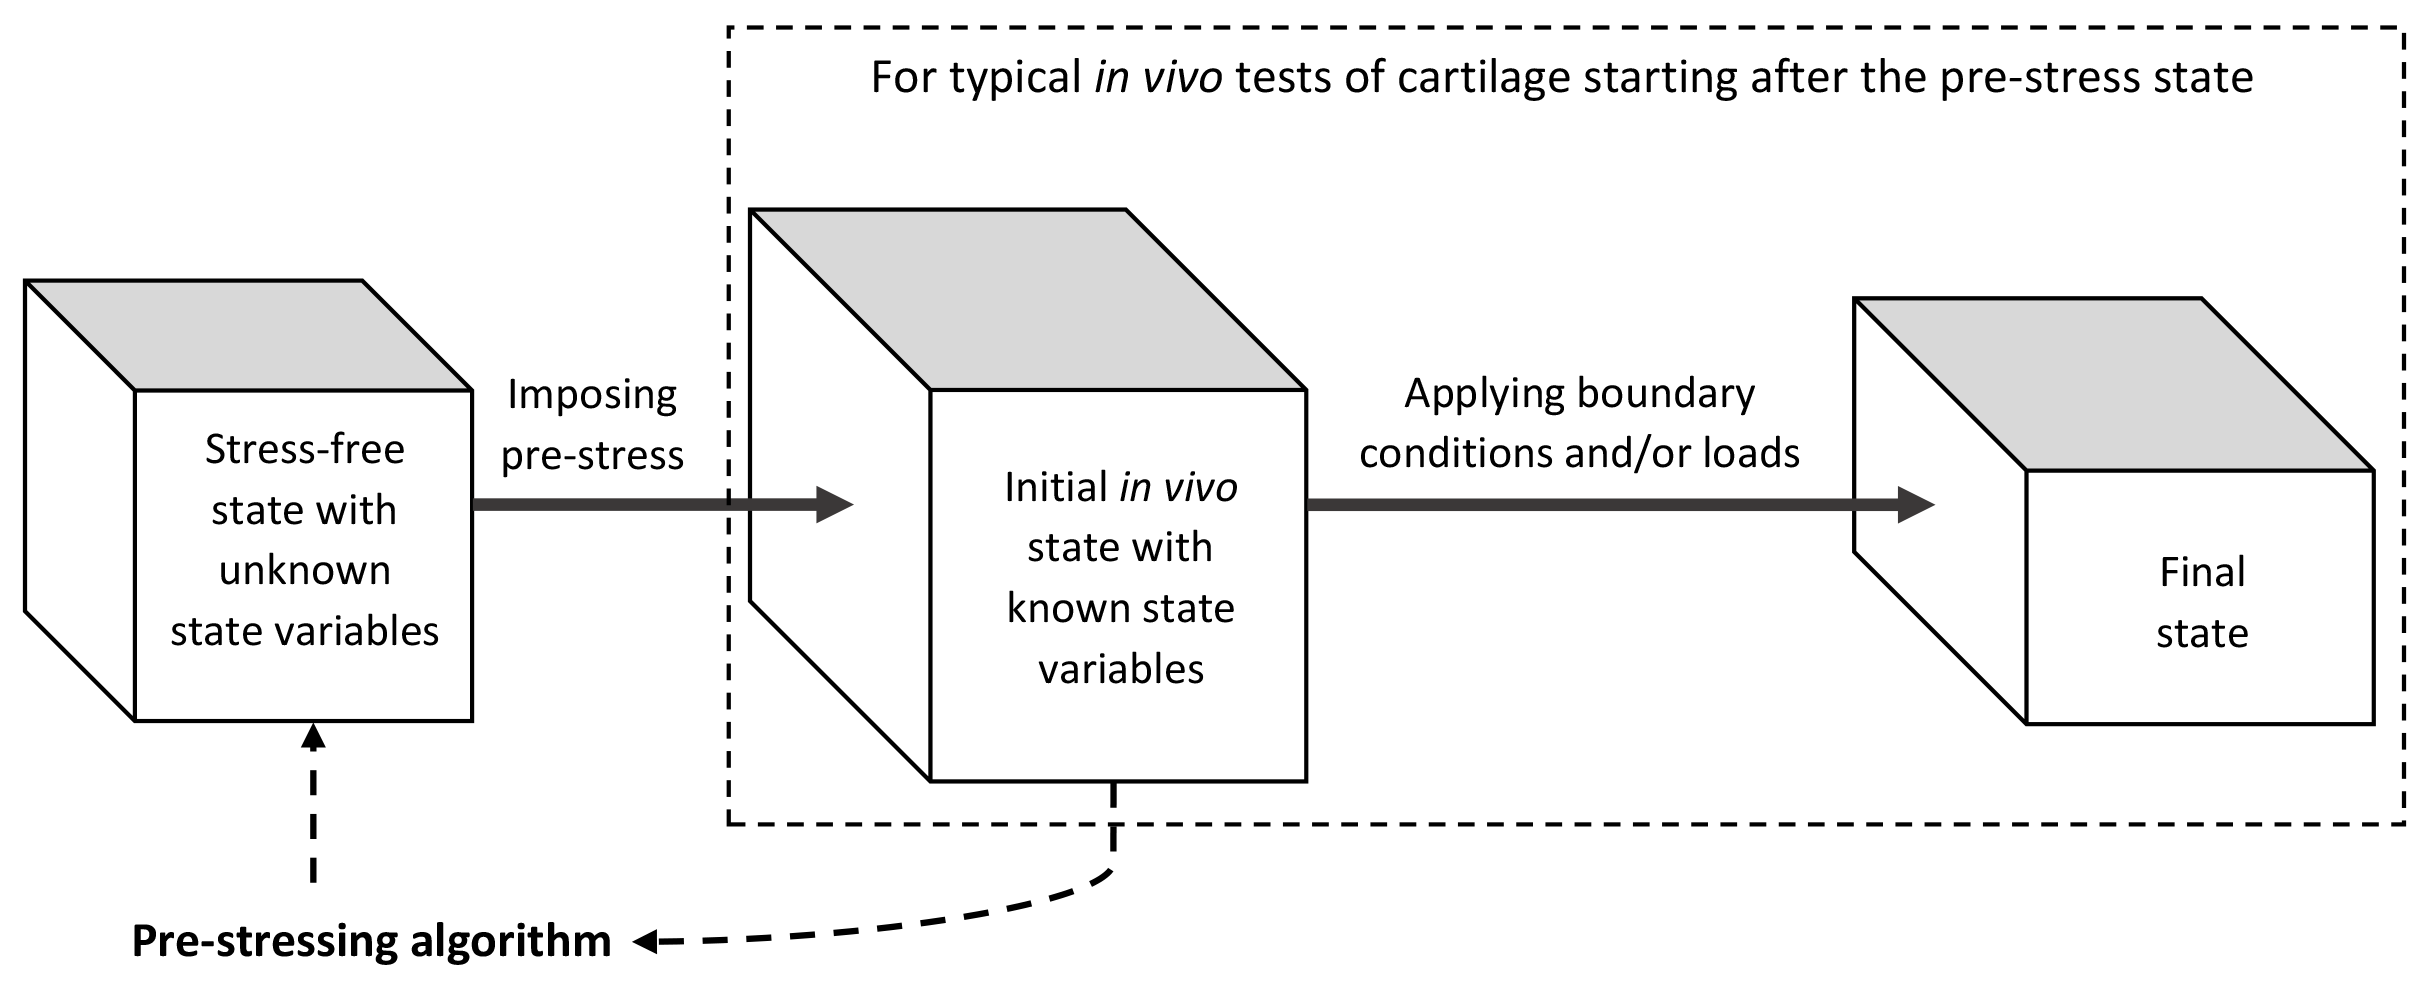
\includegraphics[width=\textwidth]{img/psa_chart.png}
%\vspace{2.5cm}
\caption{The role of the PSA in various simulation states: initially, the problem is presumed to start in a stress-free state with unknown state variables, encompassing geometrical configuration, material parameters, or both. Following the application of pre-stress, these state variables are updated to their revised values, aligning with the initial conditions of standard \textit{in vivo} or \textit{in vitro} tests that typically begin in a pre-stressed state. To ascertain the stress-free state, a PSA is employed, iteratively refining the initial estimates of state variables to align with the initial \textit{in vivo} values. Once determined, the primary numerical analysis can proceed to simulate the experimental test.}
\label{fig:psa_chart}
\end{figure}

Now, considering the initial values of the parameters influenced by pre-stressing in our numerical model, symbolized by $\mathbf{s}$, they encompass geometrical data $\mathbf{x}$ and constitutive data $\mathbf{m}$ (components include $\mathbf{n}$, $\emptyset^{\rm{S}}$, and $\rho^{\rm{COL}}$). Our \ac{psa} conducts the following sequence of analyses:
%
\begin{equation}\label{eq:optimizer}
    \mathbf{s}_{0}^{(t)} \xrightarrow[]{\text{forward analysis}} \mathbf{x}_{0}^{(t+1)} \xrightarrow[]{\text{backward analysis}} \mathbf{m}_{0}^{(t+1)}.
\end{equation}
%
The forward analysis aims to estimate the stress-free geometry, and the backward analysis determines the alterations in material properties at this state.

\paragraph{Forward analysis.} When pre-stressing is applied to the model in its initial state $\mathbf{s}^{(t)}_0$, the pre-stressed configuration $\hat{\mathbf{x}}^{(t+1)}$ is derived through an FE analysis and the multiphasics constitutive model eqs.~\ref{eq-cartilage_solid} \& \ref{eq-stress}. The update function $\mathbf{u}$ is defined as
%
\begin{equation}
    \mathbf{u}^{(t)} := \hat{\mathbf{x}}^{(t)}-\mathbf{x}^{\rm{(REF)}},
\end{equation}
%
and the stress-free geometry is edited in the following manner:
%
\begin{equation}
    \mathbf{x}_{0}^{(t+1)} := \left\{\begin{matrix}
    \mathbf{x}_{0}^{(t)} - \zeta^{(t)} \mathbf{u}^{(t)}  & \ \ \rm{if} \ \mathit{r}^{(t)} \leq \mathit{r}^{(t-1)},\\ 
    \mathbf{x}_{0}^{(t)} & \ \ \rm{if} \ \mathit{r}^{(t)} > \mathit{r}^{(t-1)},
    \end{matrix}\right.
\end{equation}
%
with $r$ and $\zeta$ being respectively the residual and scaling factor, each determined by the optimization algorithm.

\paragraph{Backward analysis.} The PSA, now, confines all the \ac{ac} nodes with the (displacement-based) boundary condition $\mathbf{b}$, using
%
\begin{equation}
    \mathbf{b}^{(t+1)} := \left\{\begin{matrix}
     - \zeta^{(t)}\mathbf{u}^{(t)} & \ \ \rm{if} \ \mathit{r}^{(t)} \leq \mathit{r}^{(t-1)},\\ 
    \mathbf{0} & \ \ \rm{if} \ \mathit{r}^{(t)} > \mathit{r}^{(t-1)}.
    \end{matrix}\right.
\end{equation}
%
This allows another (backward) FE analysis to compute the new constitutive state $\mathbf{m}_0^{(t+1)}$ using eqs.~\ref{eq:n} and \ref{eq:phi}, starting with state $\mathbf{s}_0^{(t)}$:
%
\begin{equation}
    \mathbf{n}_{0}^{(t+1)} := \frac{\check{\mathbf{F}}^{(t)}\mathbf{n}_0^{(t)}}{\left \|\check{\mathbf{F}}^{(t)}\mathbf{n}_0^{(t)} \right \|_2},
\end{equation}
%
\begin{equation}
    \varphi_{0}^{(t+1)} := \frac{\varphi_0^{(t)}}{\rm{det}\check{\mathbf{F}}^{(t)}} 
    \qquad \text{with } \forall \varphi \in \left\{\emptyset^{\rm{S}},\ \rho^{\rm{COL}}\right\}.
\end{equation}
%
In this context, $\check{\mathbf{F}}$ represents the deformation gradient in the inverse analysis, as determined by the computational solver.

\paragraph{Optimization.} With the following initial values,
%
\begin{equation}
\left\{
\begin{aligned}
    \mathbf{s}_{0}^{(0)} &:= \mathbf{s}^{\rm{(REF)}}, \\
    \mathbf{u}^{(0)} &:= \mathbf{0}, \\
    \zeta^{(0)} &:= 1, \\
    r^{(0)} &:= \infty, \\
    \mathbf{b}^{(0)} &:= \mathbf{0}, \\
    \check{\mathbf{F}}^{(0)} &:= \mathbf{I},
\end{aligned}
\right.
\end{equation}
%
the above-mentioned optimizer allows estimation of the new initial state $\mathbf{s}_{0}^{(t+1)}$, i.e., $\mathbf{x}_{0}^{(t+1)}$ and $\mathbf{m}_{0}^{(t+1)}$. This process necessitates the use of the following equations:
%
\begin{equation}\label{eq:r}
    r^{(t)} := \left \| \mathbf{U}^{(t)} \right \|_2,
\end{equation}
%
\begin{equation}
    \zeta^{(t)} := \left\{\begin{matrix}
    \zeta^{(t-1)}  & \ \ \rm{if} \ \mathit{r}^{(t)} \leq \mathit{r}^{(t-1)},\\ 
    \displaystyle \frac{\zeta^{(t-1)}}{\eta} & \ \ \rm{if} \ \mathit{r}^{(t)} > \mathit{r}^{(t-1)},
    \end{matrix}\right.
\end{equation}
%
where $\mathbf{U}$ encompasses all components of $\mathbf{u}$ at every node, and $\eta=4$ acts as a hyperparameter for averting potential divergence (adjustable for better convergence). The optimization is assumed to be converged when the error derived from eq.~\ref{eq:r} diminishes significantly, signifying the approximation of the stress-free state $\mathbf{s}_0$ is achieved through our \ac{fpbbs}.

This algorithm can be further modified by using a different residual function, such as the infinity norm, to enhance pointwise optimization. Additionally, rather than calculating volume fraction changes in backward analysis, an alternative optimizer could be employed to test various initial values, achieving a better approximation of pre-stressed values. The sequential application of constitutive and geometrical parameters may improve convergence. Despite variations in implementation, all methods adhere to the same concept of cartilage \ac{psa} with also the \ac{mo}.

\subsection{Simulation Tests}\label{section:simulation_fe}

\paragraph{Numerical Implementation.} The \ac{fe} implementation of the \ac{ac} pre-stressing, as depicted in Fig.~\ref{fig:psa_subroutines}, involves forward analyses that incorporate stress-free material properties. This is achieved via our Fortran SDVINI subroutine, responsible for setting the initial state variable values at each integration point in the numerical model. This subroutine operates in alignment with Abaqus' step 0, which determines the geometric attributes (positions) of these points. Consequently, material parameters can be initialized with respect to the normalized depth $z$, and these computed variables are further processed through our Fortran UMAT subroutine for modeling the solid components of the tissue.

\begin{figure}[t]\centering
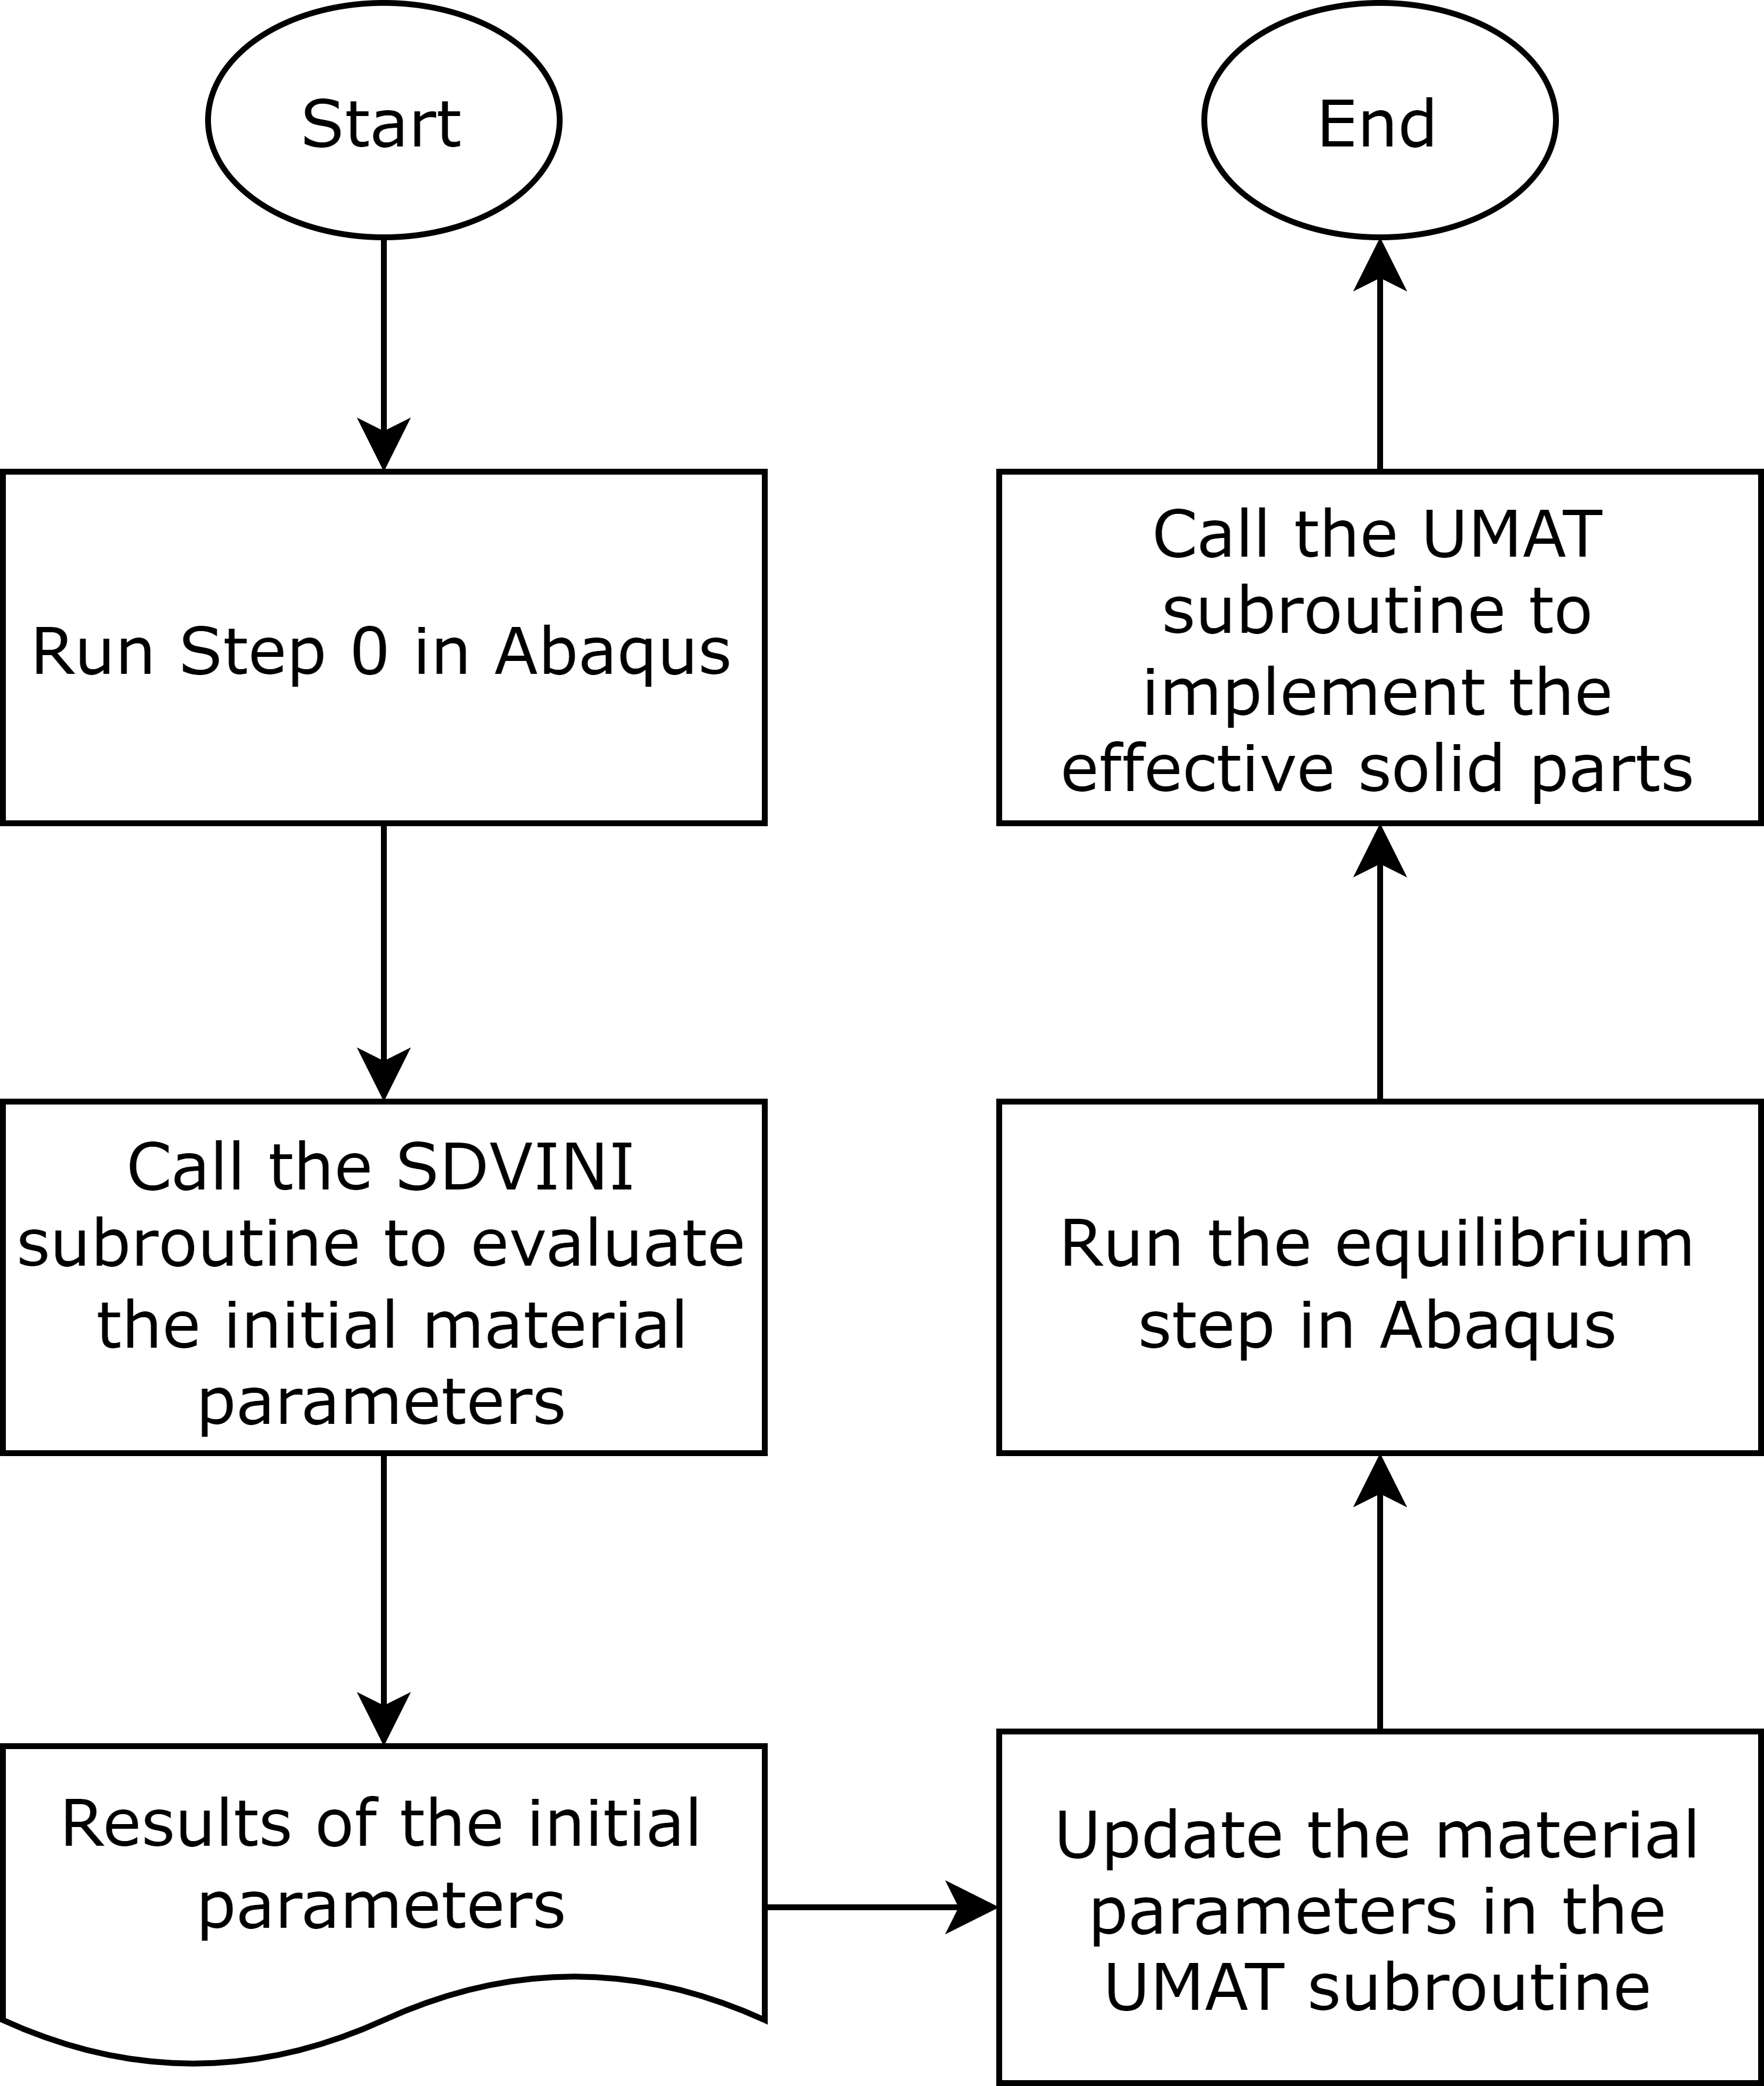
\includegraphics[width=0.5\textwidth]{img/psa_subroutines.png}
\caption{Schematic representation of the pre-stressing implementation in cartilage models, using the Fortran subroutines of Abaqus.}
\label{fig:psa_subroutines}
\end{figure}

The \ac{fpbbs}, as outlined in the preceding section, is implemented through a Python script. Initially, two FE models, mirroring each other and based on initial experimental data, are constructed for forward and inverse \ac{fe} analysis. Both models are assigned the same boundary conditions, with the inverse model incorporating also displacement nodal field $\mathbf{b}$ at each \ac{ac} node, starting at zero to represent an undeformed state.

Following the backward analysis, the newly derived parameters are reintegrated into the SDVINI subroutine to initiate a fresh cycle of \ac{psa}. This iterative process persists until convergence is attained. However, substantial variations in the updating state variables during certain iterations may hinder the FE analysis or \ac{psa} convergence, which can be managed by moderating parameter updates, albeit increasing iteration counts. Figure~\ref{fig:psa_run} illustrates the PSA implementation in Abaqus, as employed in the following simulation experiments.

\begin{figure}[t]\centering
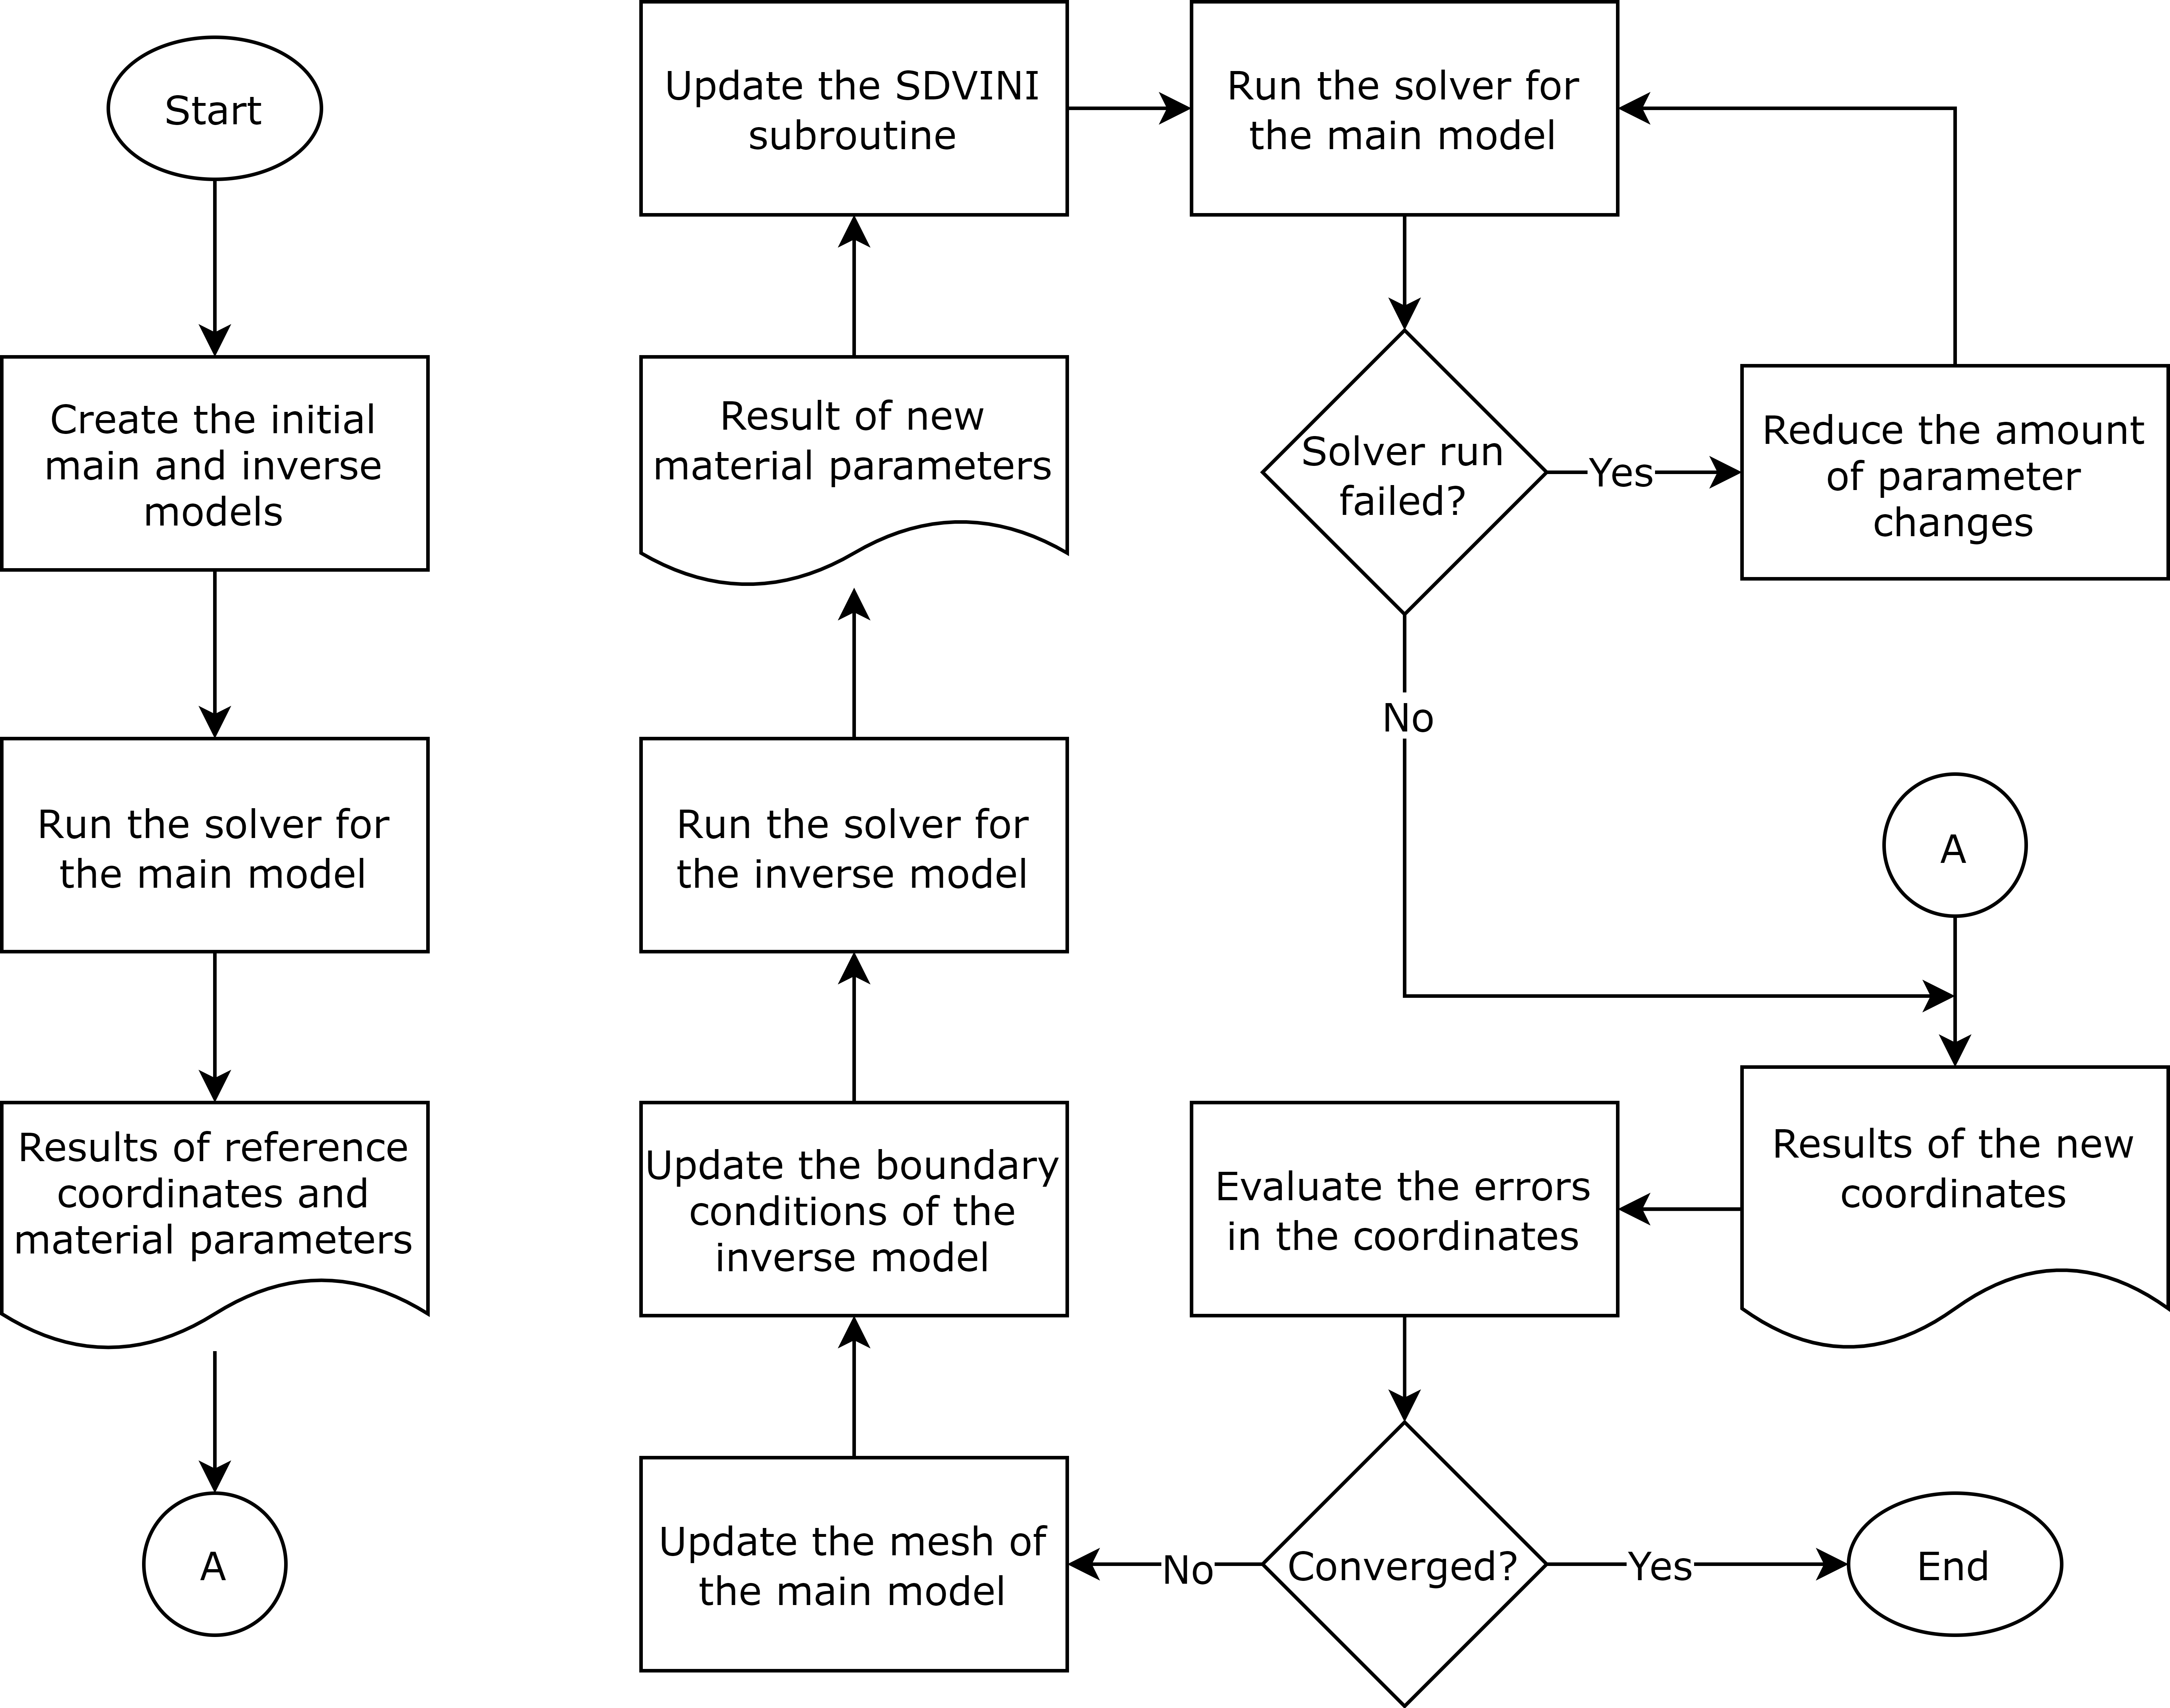
\includegraphics[width=\textwidth]{img/psa_run.png}
\caption{Flowchart of the backward optimization of our PSA, executed in Abaqus using a Python script.}
\label{fig:psa_run}
\end{figure}

\paragraph{2D tests.} Aligning with \cite{wang2018}'s earlier study on \ac{ac} pre-stressing, it is assumed that pre-stress alterations predominantly affect fibrillar component of cartilage matrix. Accordingly, tensile tests, both with and without material updates, are simulated using fully integrated 8-node biquadratic displacement and bilinear pore pressure elements. These simulations incorporate velocity boundary conditions to emulate a 1.2 stretch over 4000~Sec (refer to Fig~\ref{fig:fe_psa_2d}, right). For material calibration, a SciPy-based optimizer is employed to align FE models with varying fibrillar elasticity to empirical data [\cite{elliott2002}], using experimental stress and stretch records. The concept of experimental biomechanical parameters during pre-stressing is detailed in \cite{wang2018}'s research.
%
\begin{figure}\centering
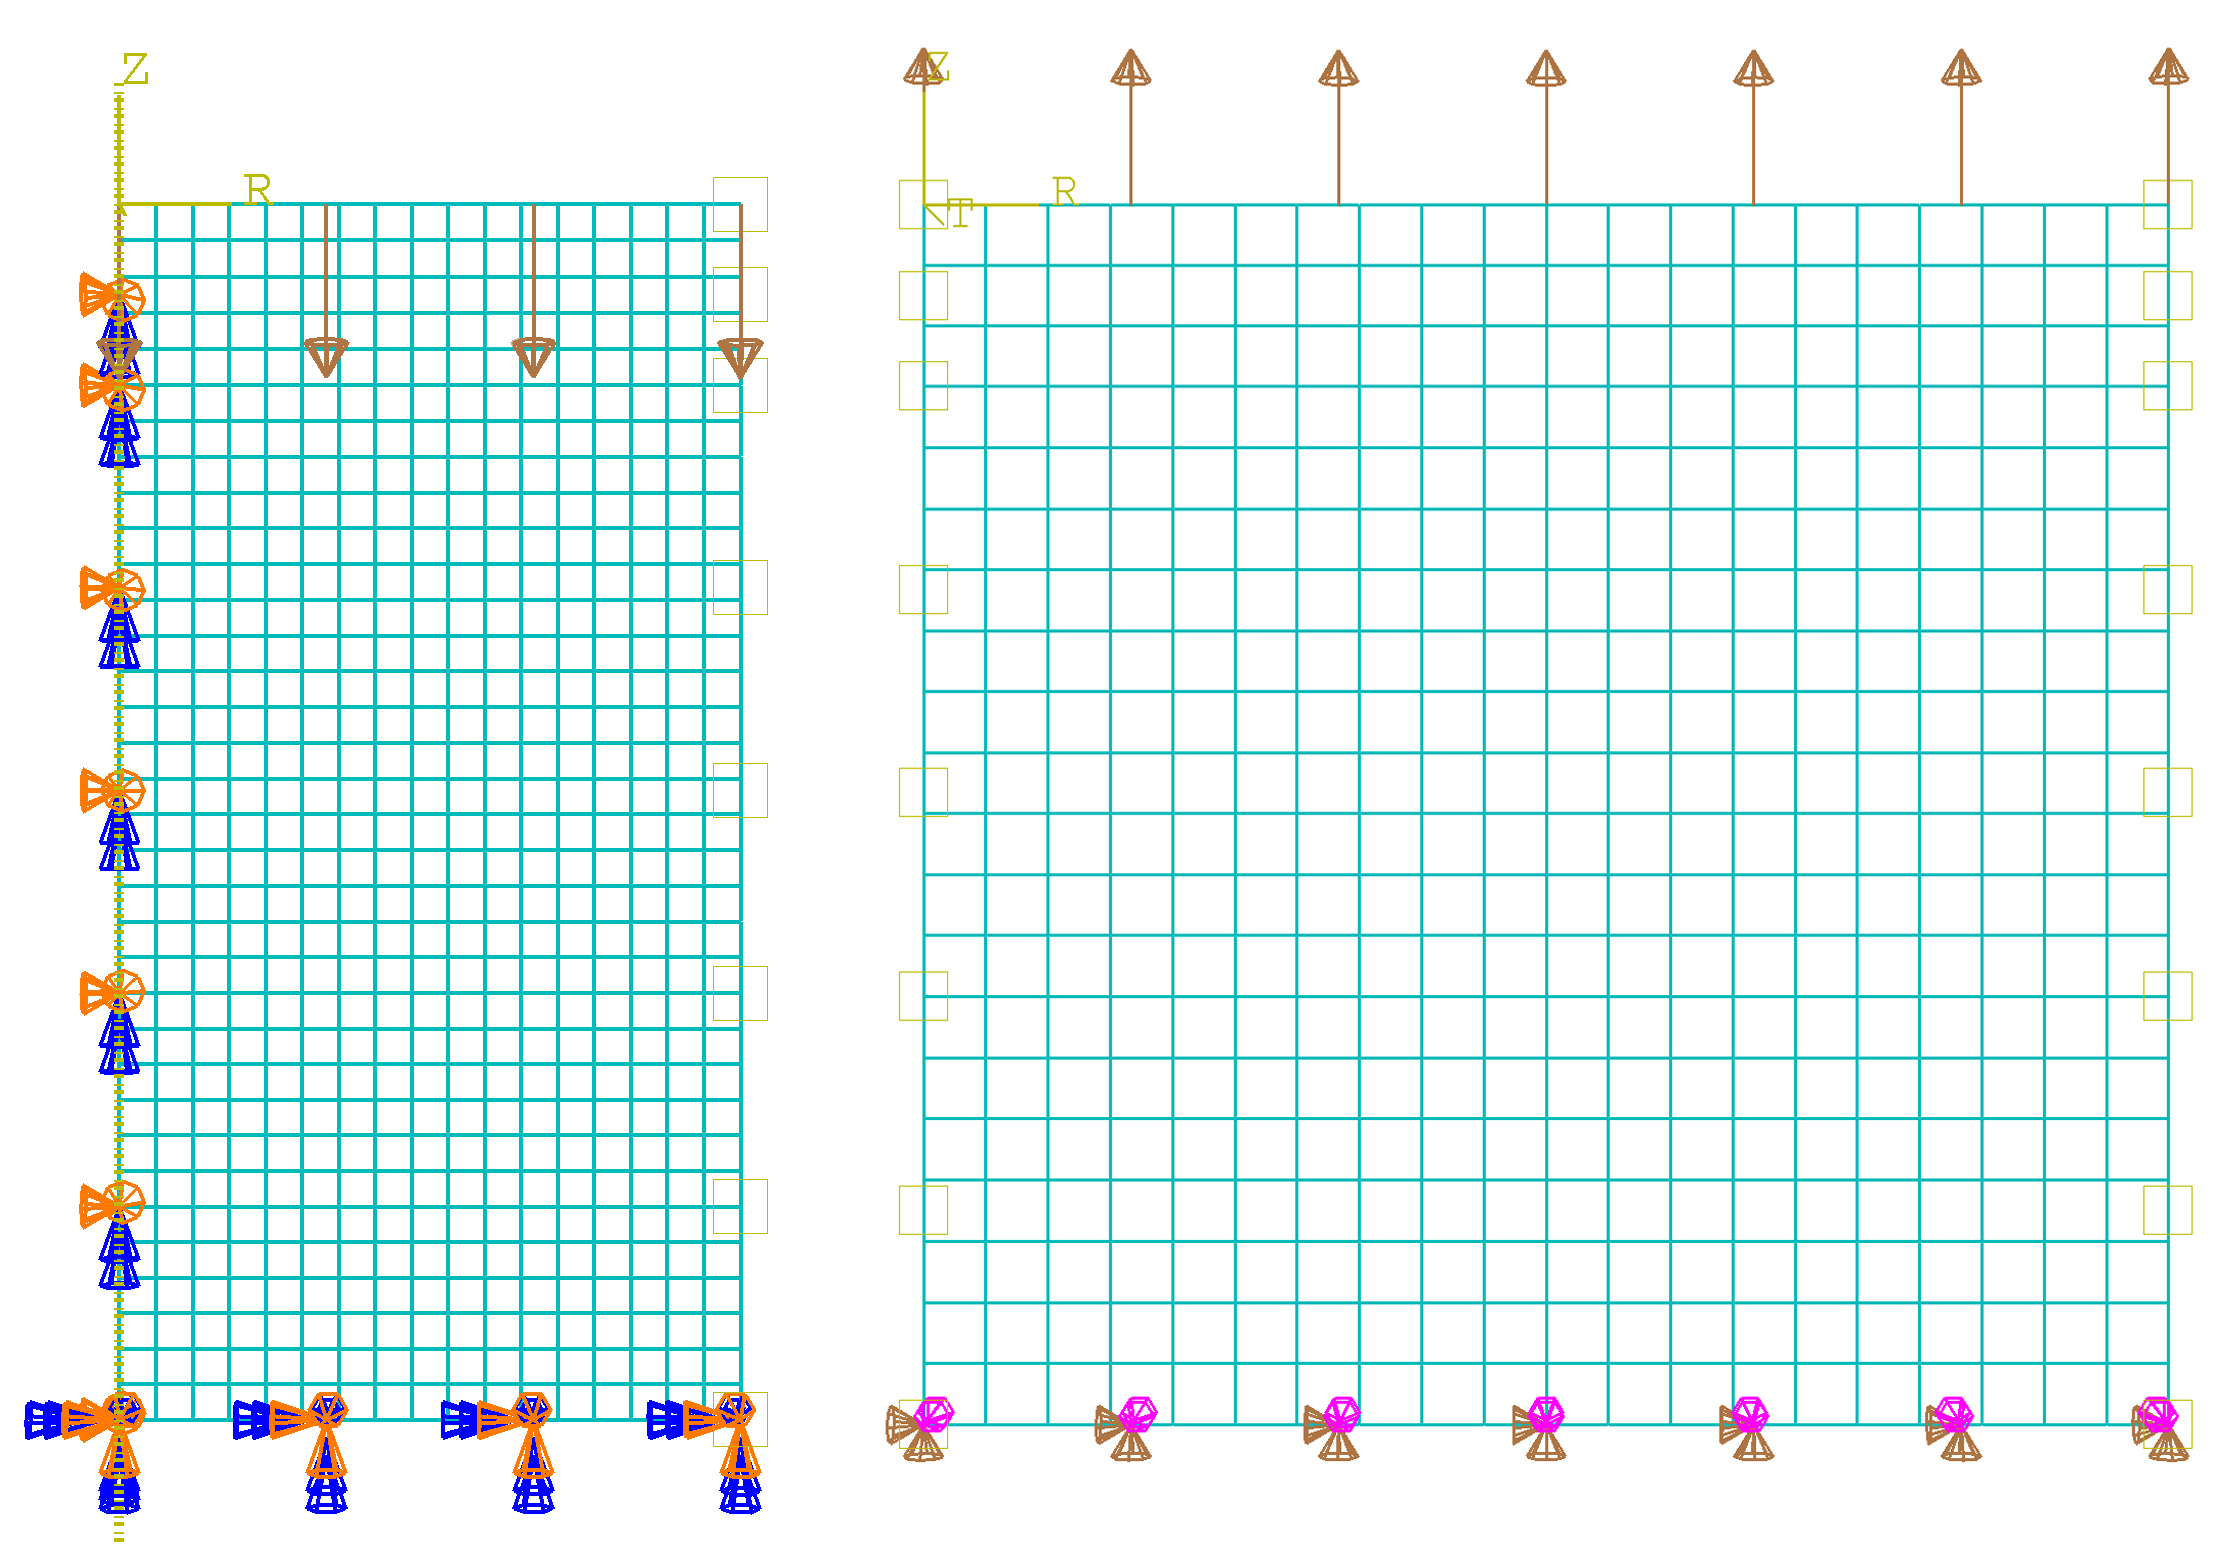
\includegraphics[width=0.7\textwidth]{img/fe_psa_2d.jpg}
\caption{2D models with an axisymmetric geometry (left) and a plane strain geometry (right).}
\label{fig:fe_psa_2d}
\end{figure}

In exploring the significance of including material parameters in pre-stressing updates, the PSA is conducted both with and without constitutive updates using an unconfined compression test. For them, fully integrated eight-node axisymmetric quadrilateral, biquadratic displacement, and bilinear pore pressure elements are selected, where the radial movement along the symmetry axis is restricted (refer to Fig~\ref{fig:fe_psa_2d}, left). Then, the alterations in material fractions along the symmetry axis and the changes in primary fibril orientations are calculated. In the following compression test, a cartilage plug of 0.5~mm radius underwent axial compression up to 10\% strain, guided by velocity boundary conditions on the upper nodes at 0.002~Sec\textsuperscript{-1}, finished by a relaxation phase.

Moreover, in all 2D simulations, the modeled cartilage has a maximum of 1~mm depth and zero fluid pressure at its outer boundaries, allowing fluid to flow freely. The nodes on the \ac{ac}'s lower surface are fixed completely to mimic the osteochondral interface.

\paragraph{3D test.} The knee model is derived from the Open Knee Project [\cite{erdemir2016}], based on MRI scans of a 70-year-old woman's cadaver. Here, the 2nd-order 3D brick elements with pore pressure equations are utilized for the cartilage models. Bones are modeled with rigid elements, and other knee components are modeled using eight-node \ac{3d} linear brick elements. Cartilage-bone and ligament-bone interfaces are tightly bound, while bones are subjected to full constraint. The material models used for the other substructures are extracted from the \cite{shim2016} study.

Additionally, for this joint-scale cartilage model, the normalized depth $z$ definition is redefined to accommodate the knee models with varying thicknesses. The position of each point is used to find the nearest nodal coordinates on the \ac{ac}'s upper and lower surfaces (signified by $d_t$ and $d_b$, respectively), with the aid of a nearest neighbor search algorithm [\cite{maneewongvatana1999}]. Then, 
%
\begin{equation}
    z = \frac{ d_t }{ d_t+d_b }.
\end{equation}
%
\begin{figure}\centering
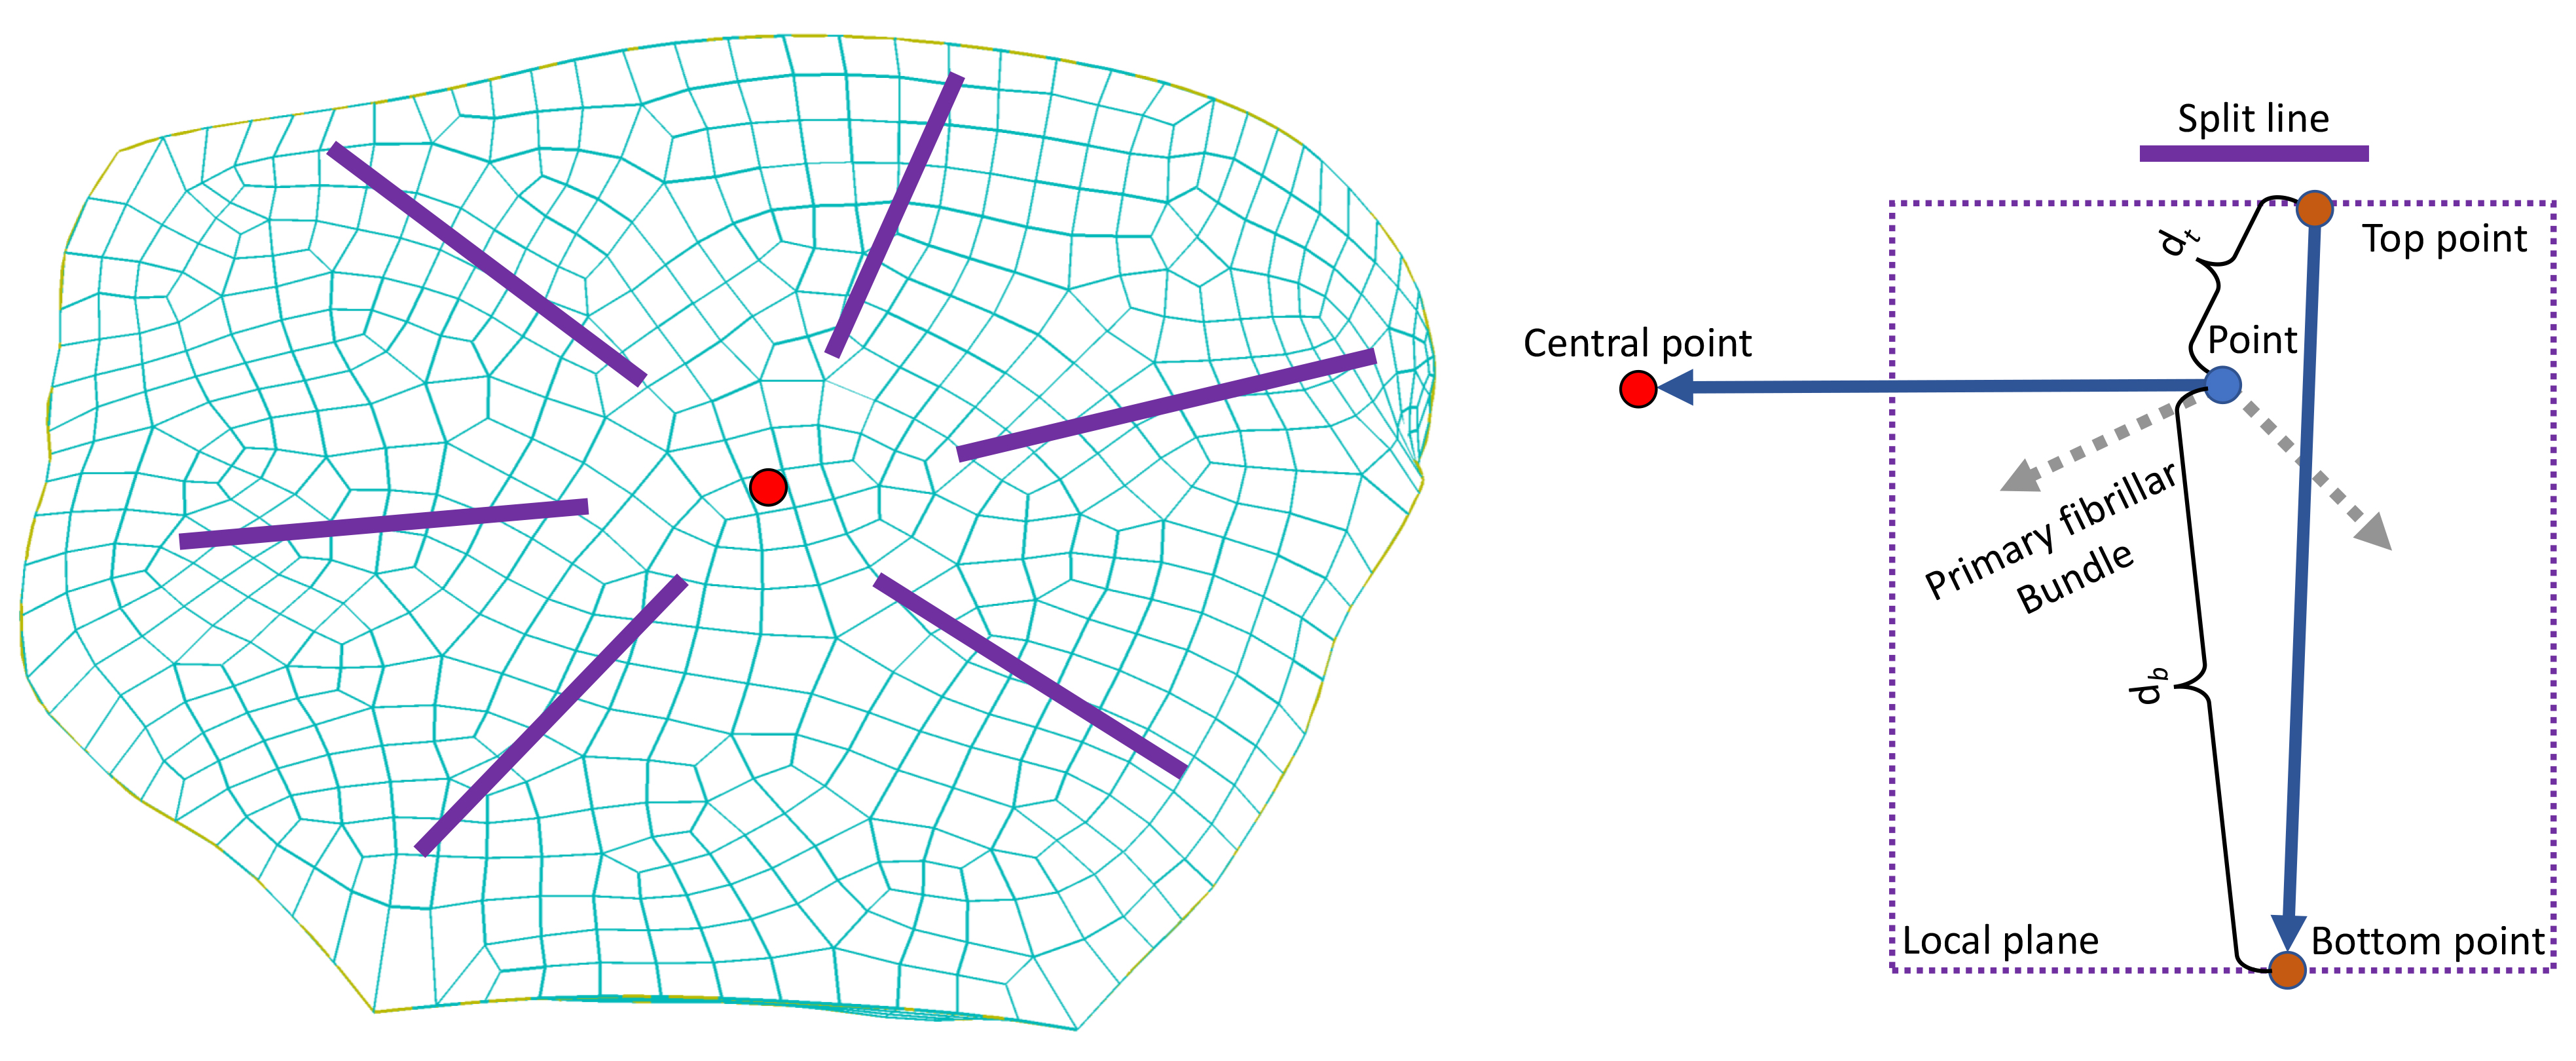
\includegraphics[width=\textwidth]{img/direction.jpg}
\caption{Example of the orientations of split lines of an AC substructure (left) and a local plane corresponding to an AC point (right).}
\label{fig:split_lines}
\end{figure}
%
Now, considering the model's asymmetry, a local plane is constructed at each \ac{ac} point, assuming that the primary fibrils within this plane mark the split-lines patterns on the AC surface. These lines are generally assumed to be directed toward the center of each cartilage substructure [\cite{mononen2012}]. Therefore, the local plane encompasses one vector facing the central point and another linking the nearest surface points, as shown in Fig.~\ref{fig:split_lines} with blue arrows. With this plane and the calculated normalized depth, the fibrillar orientations are defined, in the same way as the ones used in 2D models, complementing the \ac{fe} implementation. The code of the large-scale model is open-sourced\footnote{\href{https://github.com/shayansss/psa}{https://github.com/shayansss/psa}.} due to its complexity.

\section{Results and Discussion}
%
In this study, we introduce a novel \ac{psa} that integrates nodal geometric optimization and material optimization (MO) for \ac{fe} analysis. This approach is applied to an anisotropic, depth-dependent \ac{ac} mixture model, which comprises all major multiphasic components explained in the previous chapter. Our proposed solution addresses the inconsistency between actual \textit{in vivo} states and numerically-implemented pre-stressed states. This is achieved by incorporating constitutive variables into existing \acp{fpbbs} [\cite{wang2018,bols2013,pandolfi2008}] and by defining an inverse analysis for inclusion of these variables.

The main hypothesis of this study is that the heterogeneous constitutive properties of the multiphasic \ac{ac} model can be modified through the application of  pre-stressing via a \ac{fpbbs} with material variations, and this modification can influence the biomechanics of the tissue. To evaluate this hypothesis, a series of 2D tests was conducted, followed by a larger-scale analysis involving a tibiofemoral joint to examine the effects of pre-stressing. The proposed algorithm proved its high efficiency, as it automatically identifies the stress-free state within a maximum of six hours using a regular hardware setup in the most resource-intensive model (used in the 3D test).

\paragraph{2D tensile test.} The constitutive equations, previously validated [\cite{sajjadinia2019}], were not previously combined with pre-stressing methods. Therefore, we simulated a series of tensile tests, both with and without material variation across a broad spectrum of fibrillar elasticity parameters. The initial parameter values were based on earlier research [\cite{wilson2007}]. Table~\ref{table:calibraion} presents the derived values for both scenarios, and Fig.~\ref{fig:calibration} compares the simulation results with experimental data [\cite{elliott2002}].
%
\begin{table}[b!]\centering
\caption{Fitted constitutive parameters of the fibrillar network for the different implementations of \acp{psa}.}
\label{table:calibraion}
\begin{tabular}{lcc}
\hline
\textbf{Parameter}  
& \textbf{PSA with MO}
& \textbf{PSA without MO}
\\
\hline
$E_1$ (MPa) 
& 19.51&    30.21 
\\
$E_2$ (MPa) & 230.67&    234.11 \\
\hline
\end{tabular}
\end{table}
%
\begin{figure}\centering
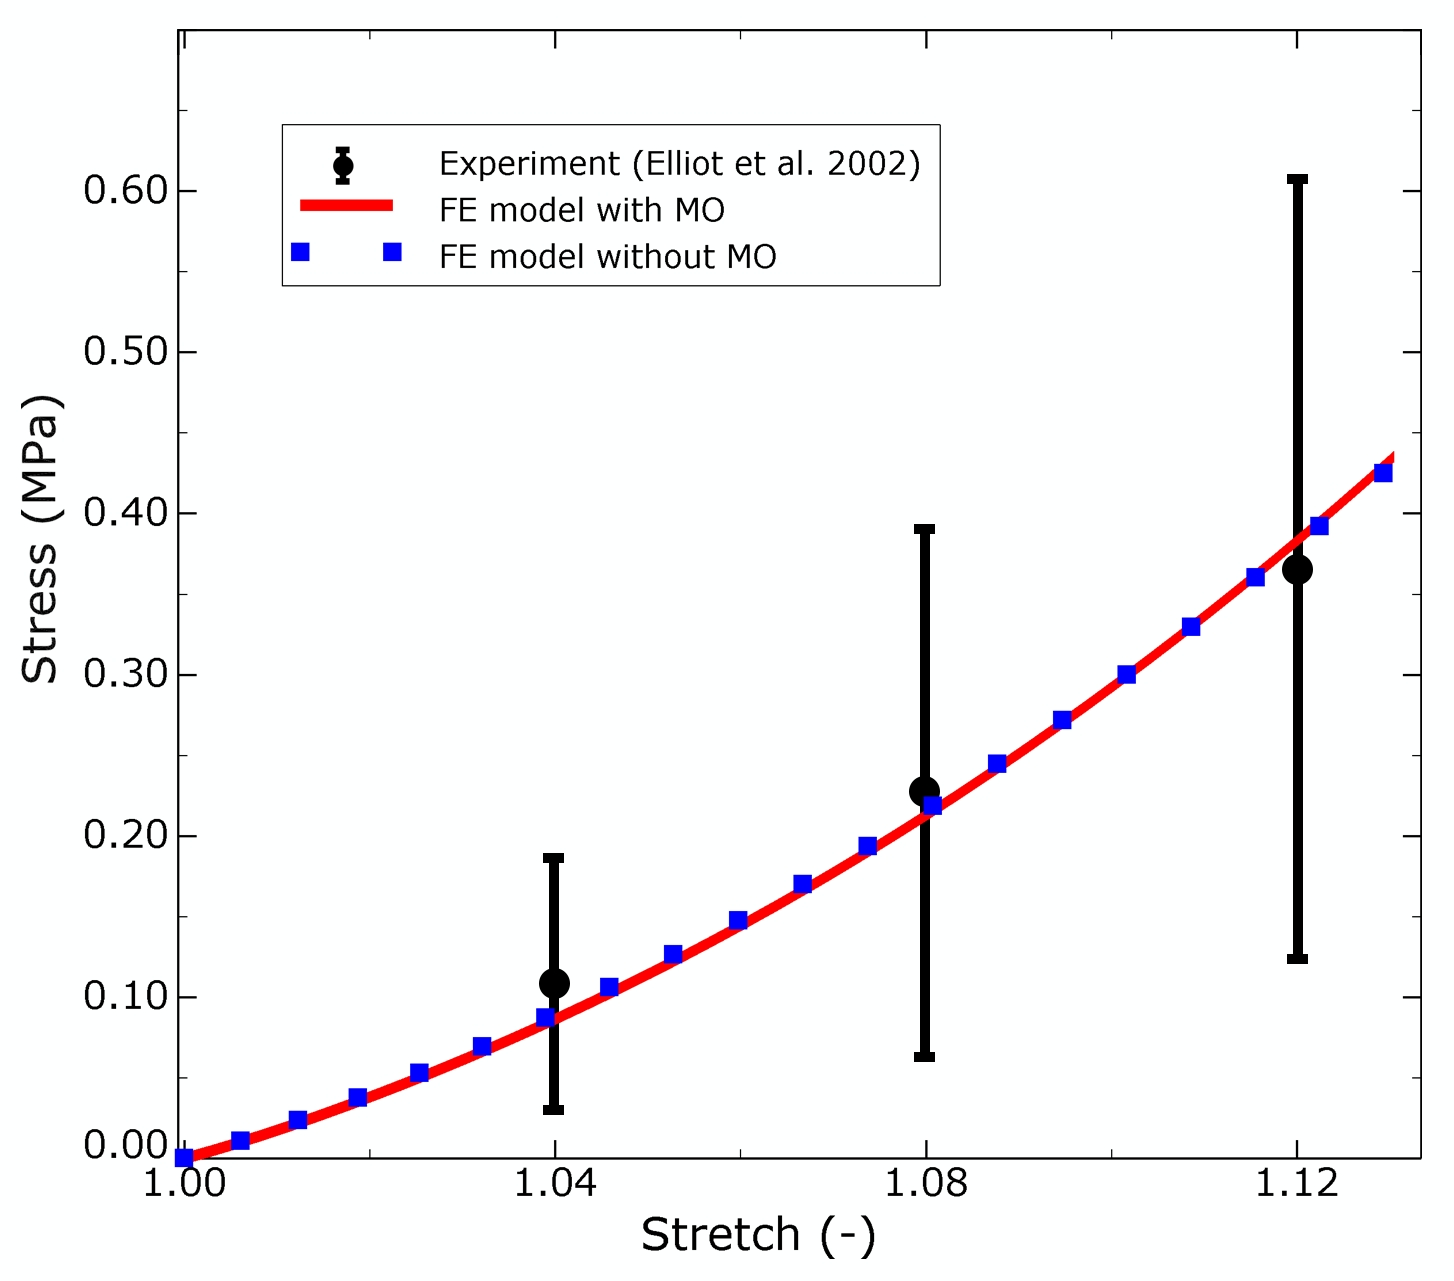
\includegraphics[width=0.5\textwidth]{img/calibration.jpg}
%\vspace{2.5cm}
\caption{Recorded stress vs. stretch extracted from calibrated numerical models mimicking an experimental test [\cite{elliott2002}].}
\label{fig:calibration}
\end{figure}

Both calibrated FE models exhibited close alignment with median values: initially, the stress-strain curves show mild nonlinearity, reflecting the cartilage's near-linear behavior at the onset. However, these curves slightly underestimate stress compared to median experimental values. At a stretch value of approximately 1.06, the response became dominated by the nonlinear elasticity of fibrils, leading to a minor overestimation of stress. Nonetheless, both recorded responses fall within the range of experimental data, indicating their applicability in general \ac{ac} modeling.

Regardless of the similarity in the results, the model without material alteration displayed slightly more strain-related fibrillar elasticity $E_2$ but significantly higher initial elasticity $E_1$. This observation could be attributed to the initial pre-stressing state where the fibrillar network predominantly resists osmotic pressure [\cite{quiroga2017}]. Also, since the model without MO has decreased material fractions, as per eq.~\ref{continuity}, there is a need to increase fibrillar elasticity, particularly the initial elasticity, to compensate for these reductions, especially at the small deformation.

\paragraph{2D compression test.} In pursuit of validating our hypothesis, we conducted \ac{fe} simulations in a confined compression scenario. These simulations were executed with previously calibrated constitutive models, both with and without optimizing the material parameters via the \acp{psa}. Accordingly, Fig.~\ref{fig:fiber_orientation} displays the distribution of the angle $\uptheta$, signifying the deviation between the radial axis and one of the exemplified fibrillar directions upon achieving equilibrium. The model incorporating \ac{mo} exhibited precise alignment with \textit{in vivo} observations. In contrast, the model lacking \ac{mo} deviated in the peripheral regions, with angle variations between 5 and 10\% compared to the \textit{in vivo} measurements.
%
\begin{figure}\centering
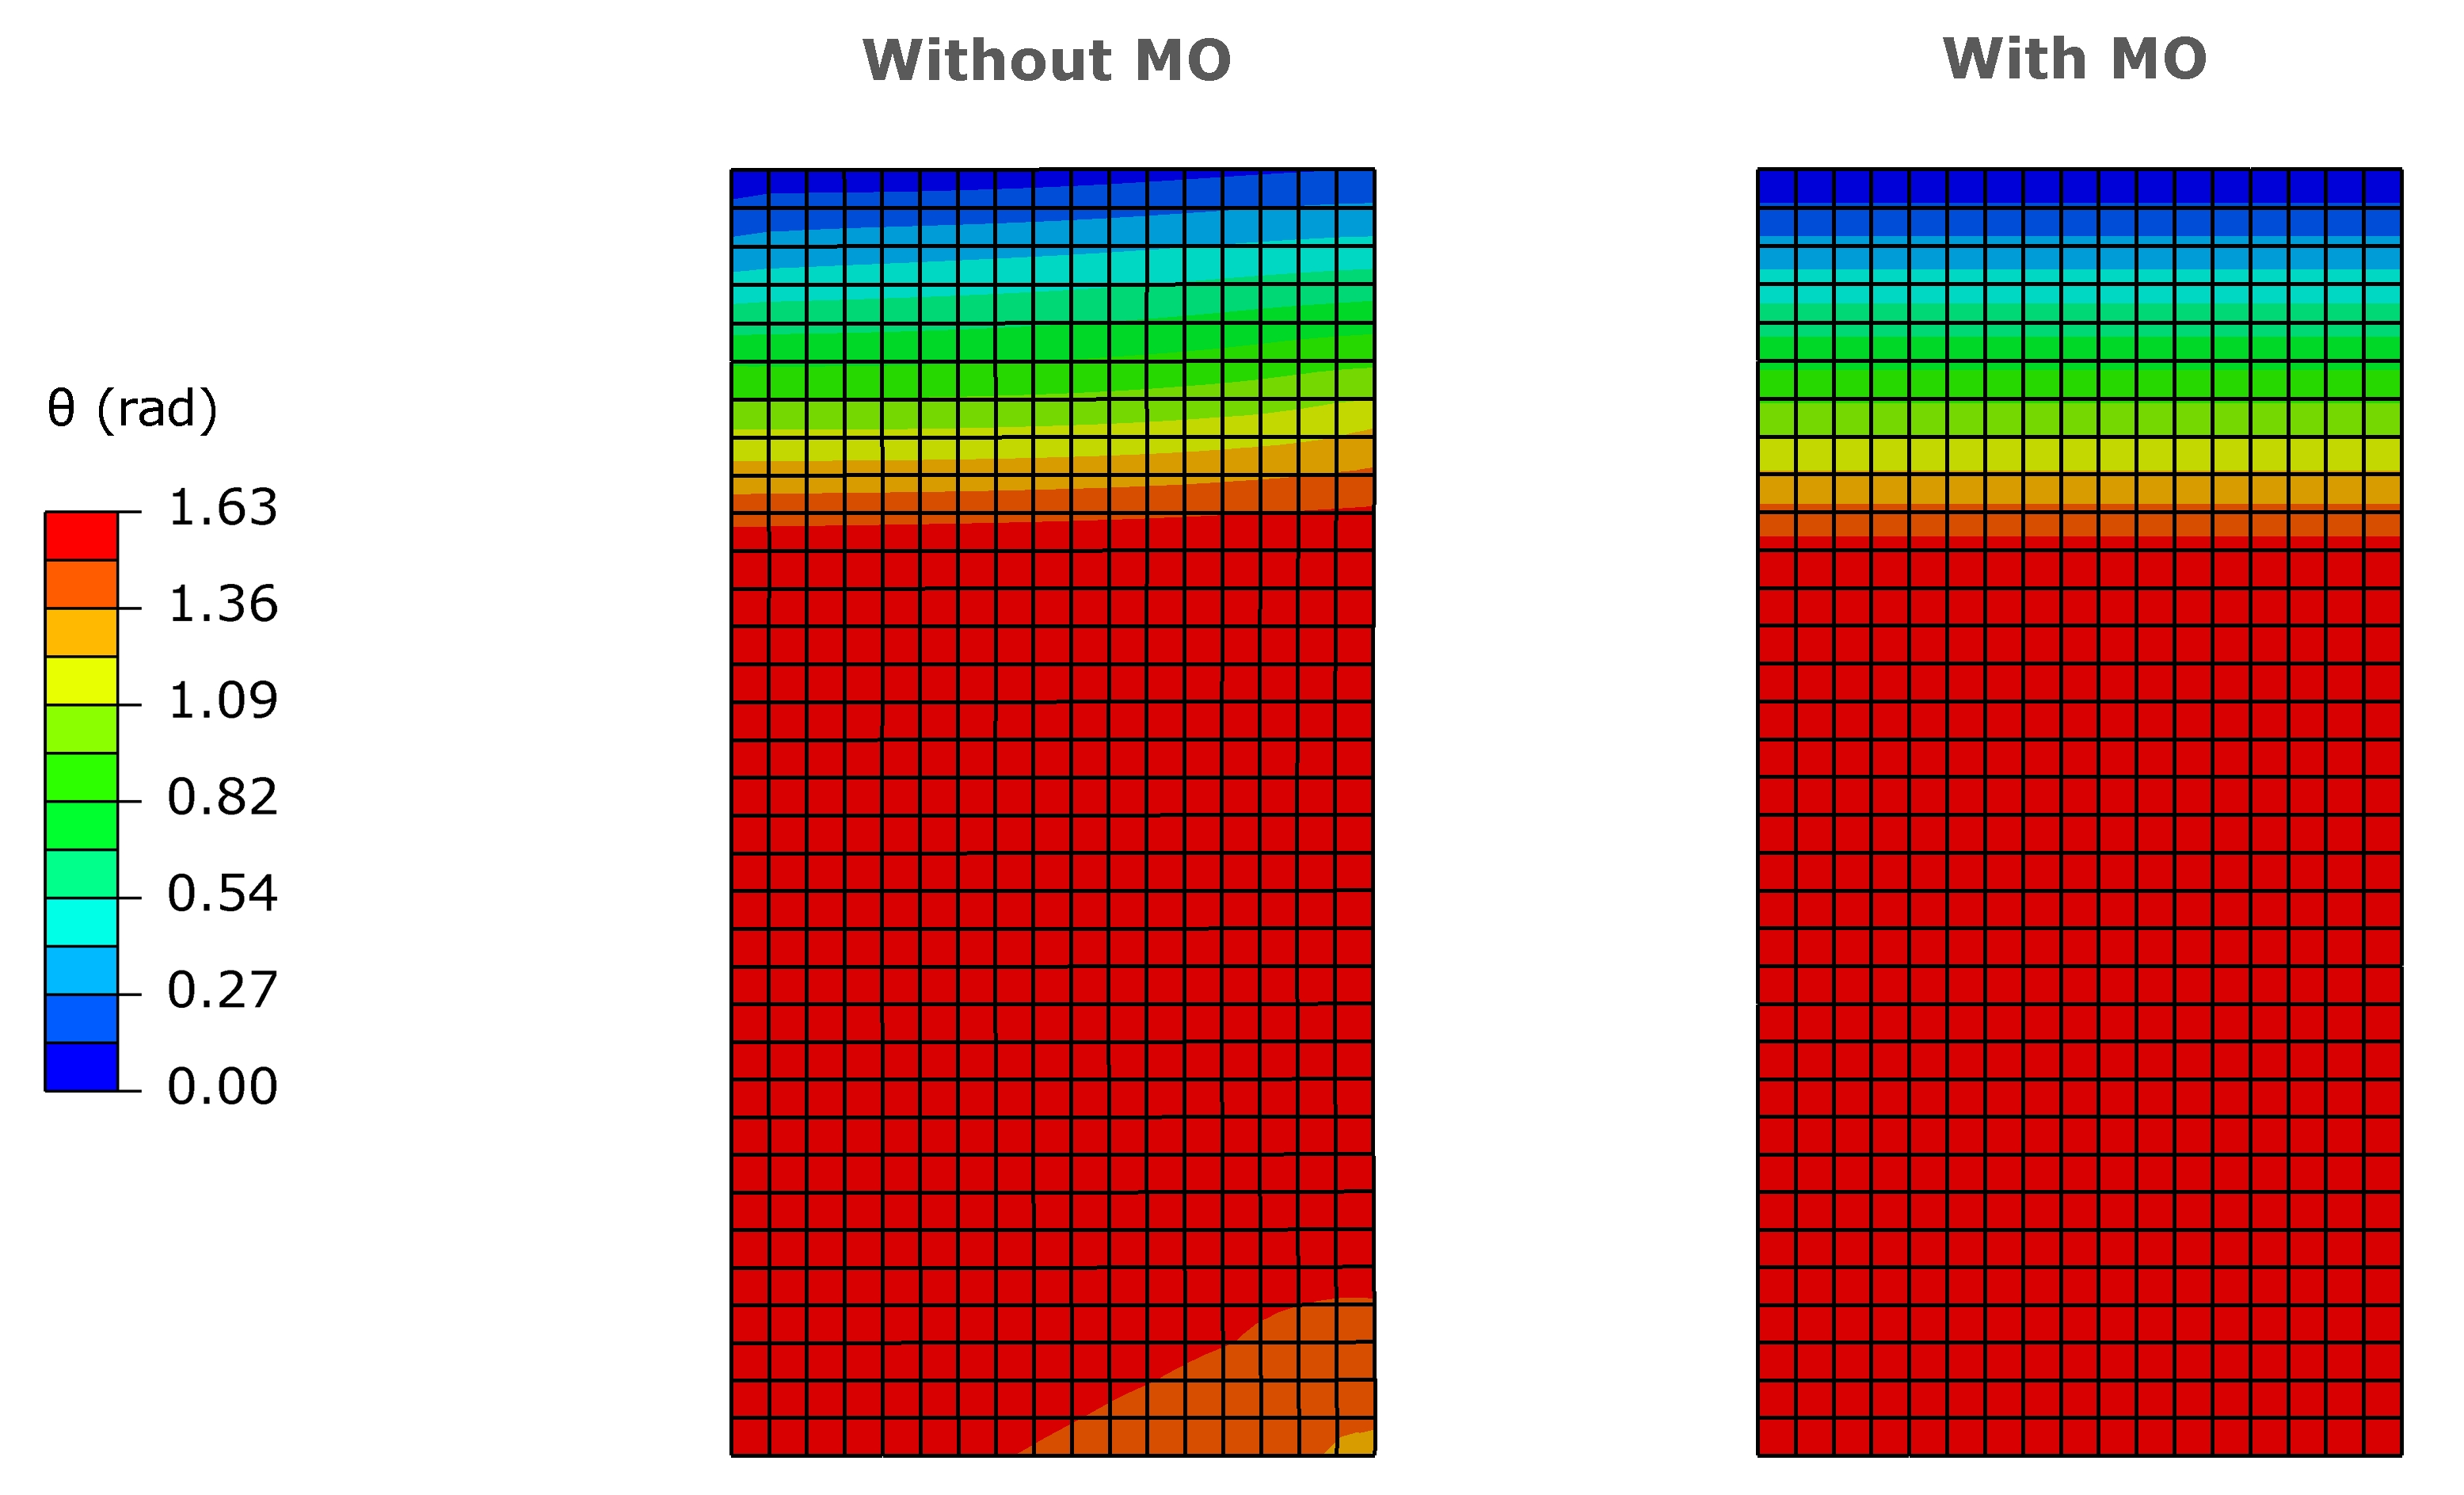
\includegraphics[width=0.7\textwidth]{img/fiber_orientation.jpg}
%\vspace{2.5cm}
\caption{Contour of a representative fibrillar angle $\uptheta$  with respect to the radial axis in pre-stressed initial states.}
\label{fig:fiber_orientation}
\end{figure}

Figure~\ref{fig:fractions} displays the variations in the volume fractions of the constitutive equations along the normalized depth in the cartilage's axis of symmetry. While both models demonstrated analogous trends, the non-\ac{mo} model exhibited approximately 8 to 16\% divergence from the experimental values across most regions; however, the deeper zones showed convergence in both models. Discrepancies in such constitutive parameters support this study's hypothesis, considering that they indicate the influence of \ac{mo} on the biomechanics of cartilage. Supporting this, \cite{julkunen2008} noted that variations in volume fractions significantly impact mechanical responses while maintaining underlying trends. These findings indirectly validate the enhanced precision and significance of \ac{mo} incorporation in \ac{psa}. Further insights into the biomechanical effects are being explored through the following relaxation test simulations.
%
\begin{figure}[b!]\centering
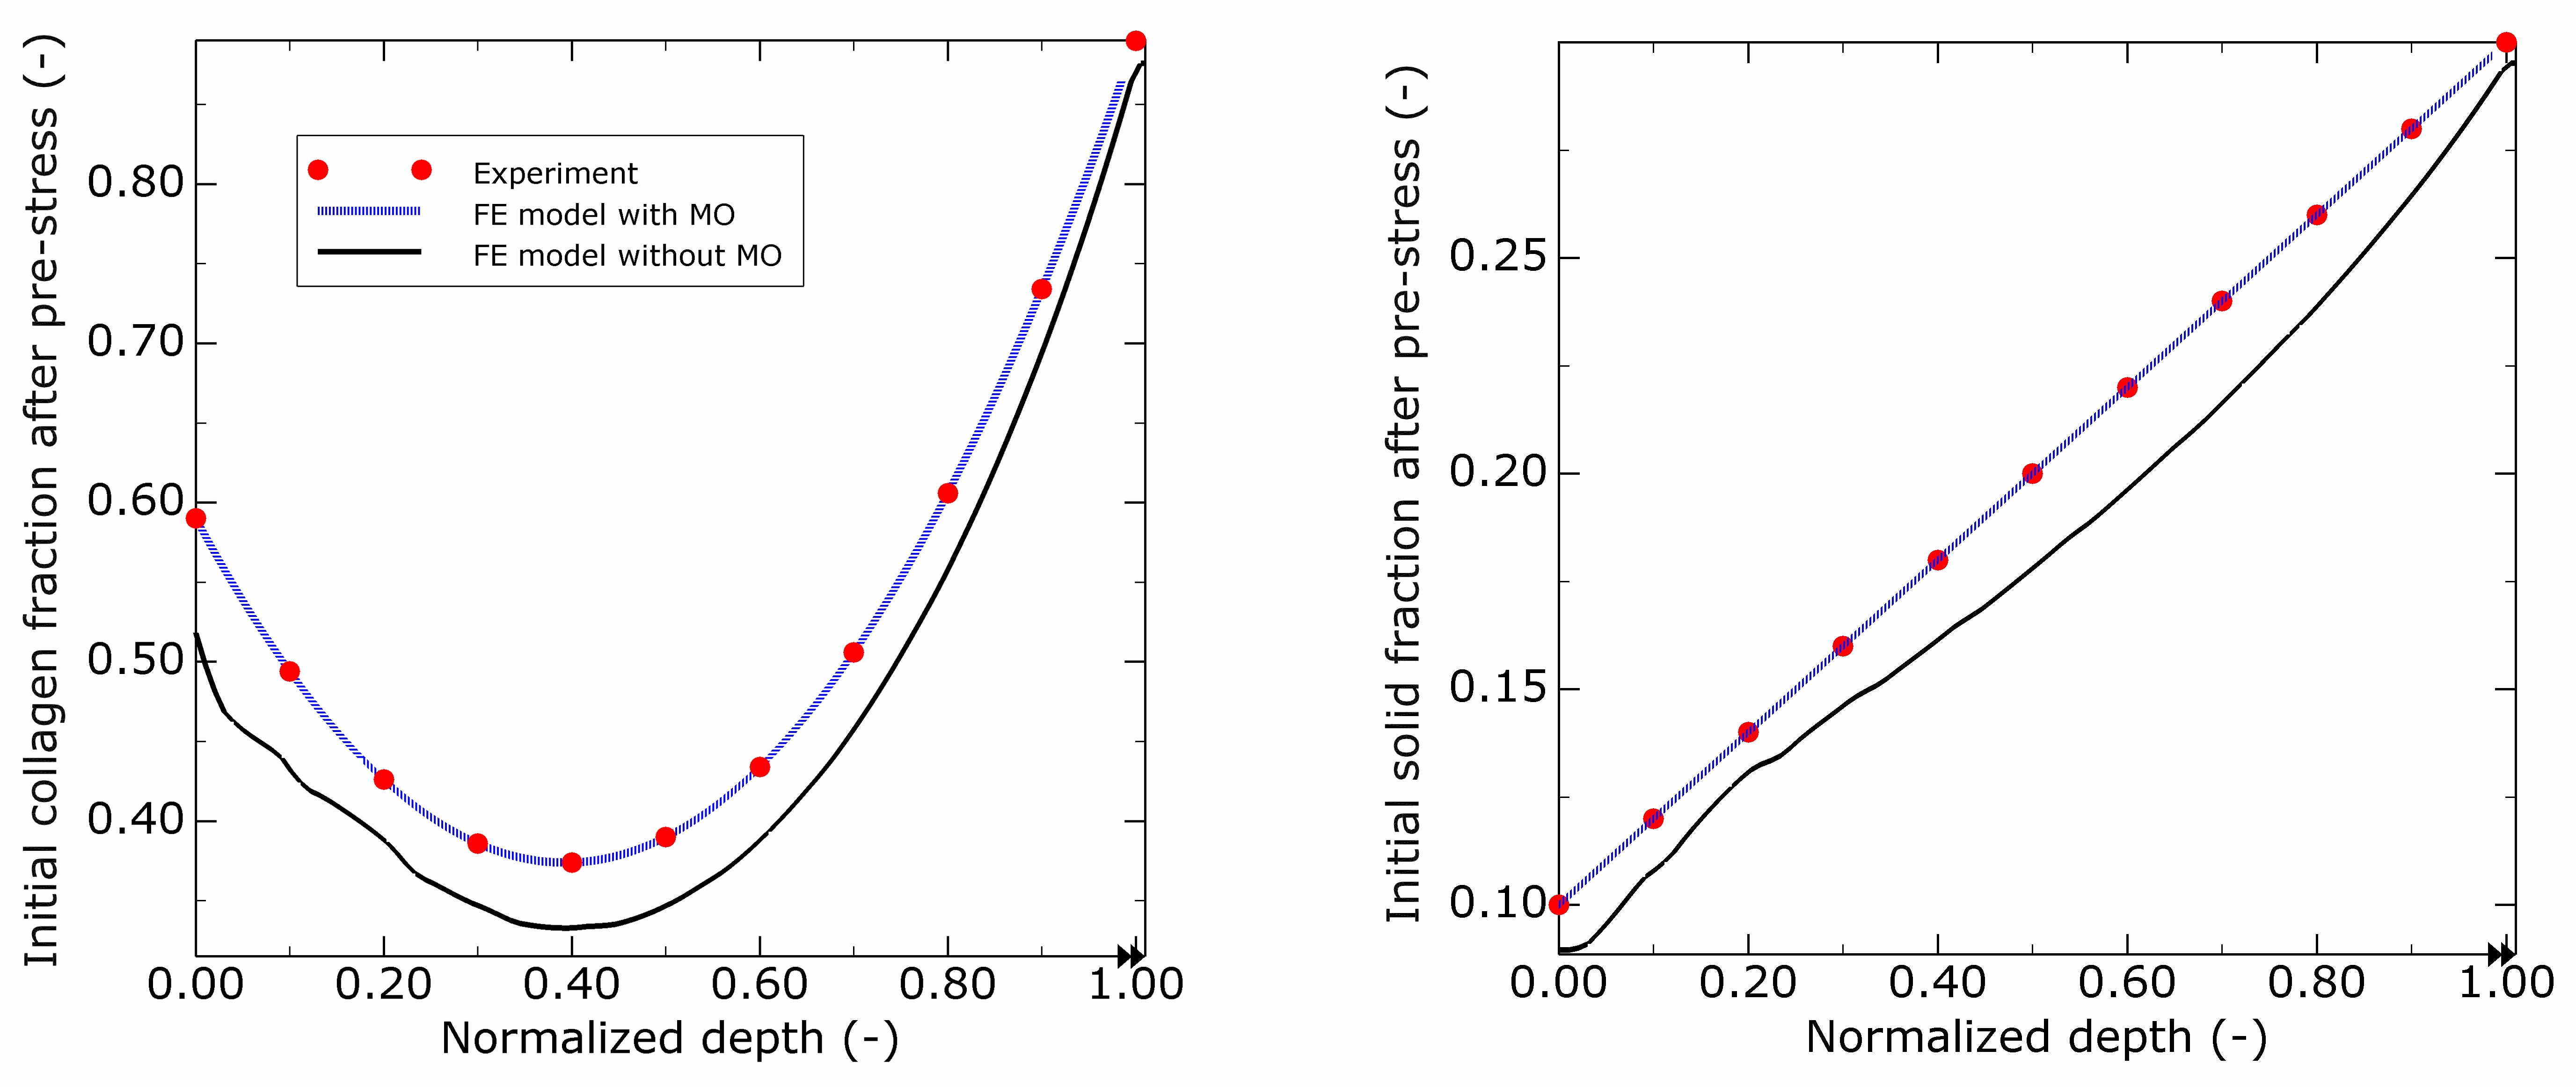
\includegraphics[width=\textwidth]{img/fractions.jpg}
\caption{Comparative plots of volume fractions with respect to the \ac{ac} normalized depth in the pre-stressed initial state compared with the experimental values [\cite{wilson2007,rieppo2004,shapiro2001,lipshitz1975}]. }
\label{fig:fractions}
\end{figure}

The axial stress-strain relationships of the solid constituents in cartilage zones were presented in Fig.~\ref{fig:parts_stress_strain}. These zones include the \ac{sz}, \ac{mz}, and \ac{dz}. At the maximum loading point, the fibrillar component exhibited a stress response change, up to 44\% when mo was incorporated, increasing from 0.42 to 0.71MPa in the \ac{mz}. In the other zones, these changes were 9\% and 12\% in the \ac{sz} and \ac{dz}, respectively. Regarding the other solid components, the non-fibrillar part showed the highest stress variation, approximately 16\%. Thus, the application of \ac{mo} resulted in notably different stress calculations compared to traditional backward algorithms, highlighting \ac{mo}'s impact on the mechanics of the tissue and further supporting our hypothesis.
%
\begin{figure}\centering
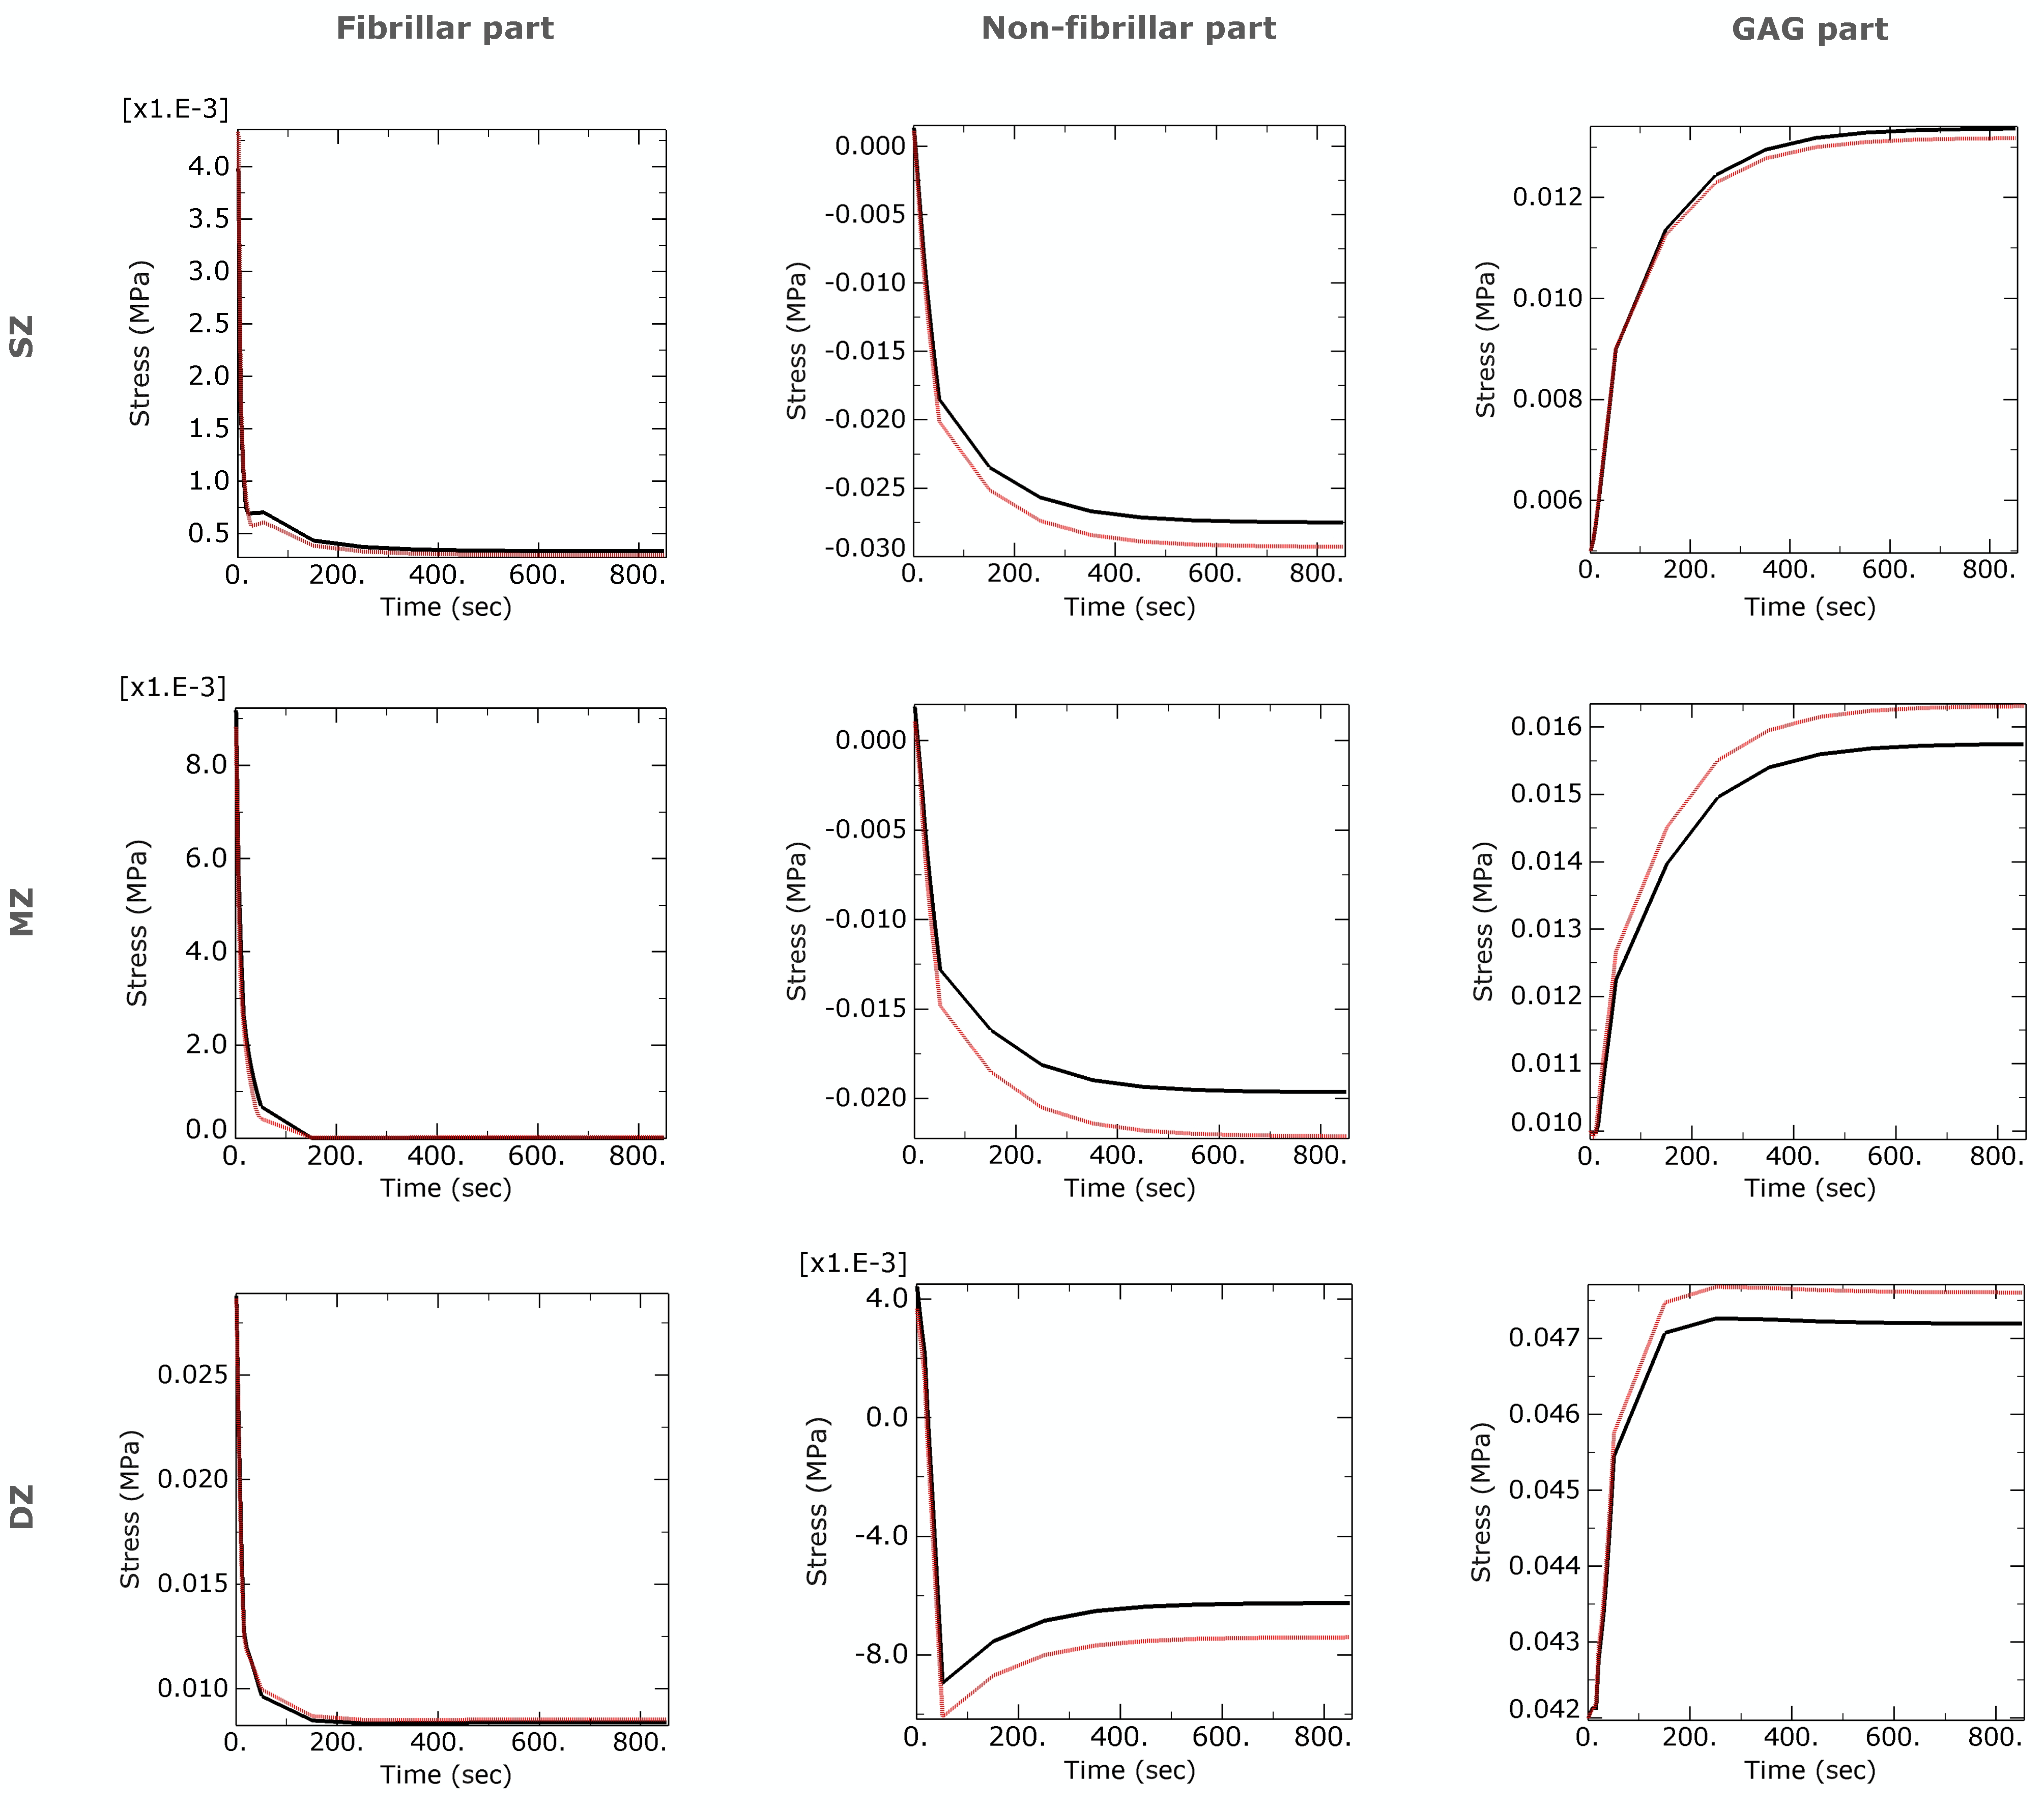
\includegraphics[width=\textwidth]{img/parts_stress_strain.jpg}
%\vspace{2.5cm}
\caption{Stress vs time plots from numerical simulations of unconfined compression experiments with (black curves) and without (red curves) \ac{mo} for different cartilage zones and effective solid parts after equilibrium.}
\label{fig:parts_stress_strain}
\end{figure}

Moreover, the stresses recorded in the constituents in the compression experiment for both models showed similar patterns, consistent with previous findings: the osmotic pressure was a major contributor to load resistance, paralleling earlier research by \cite{quiroga2017}; the fibrillar components initially exhibited high stress values, then stabilized to negligible levels, akin to observations in the \cite{wilson2007} study; notably, the stress in the fibrillar network in \ac{dz} was significantly higher than the values in other zones, explained with the higher osmotic pressure and the predominant axial orientation of primary fibrils, enhancing their contribution to axial load resistance.

Figure~\ref{fig:total_stress_strain} presents the corresponding total stress-strain curves, where both \acp{psa} yielded comparable patterns across different cartilage zones. However, minor but noticeable differences were observed, particularly during the relaxation phase, where \ac{fe} volume changes influenced volume fraction errors. The \ac{mo} effect was more obvious in the \ac{dz}, especially during relaxation, showing about a 12\% variation in strain magnitudes. These variations in the \ac{sz} and \ac{mz} were under 9\%. These particular results demonstrate the comparable accuracy of both methods, although the differences could be significant in \ac{hf} models where stress-strain data correlation is critical [\cite{eskelinen2019,liu2020,stender2016,hosseini2014}].
%
\begin{figure}
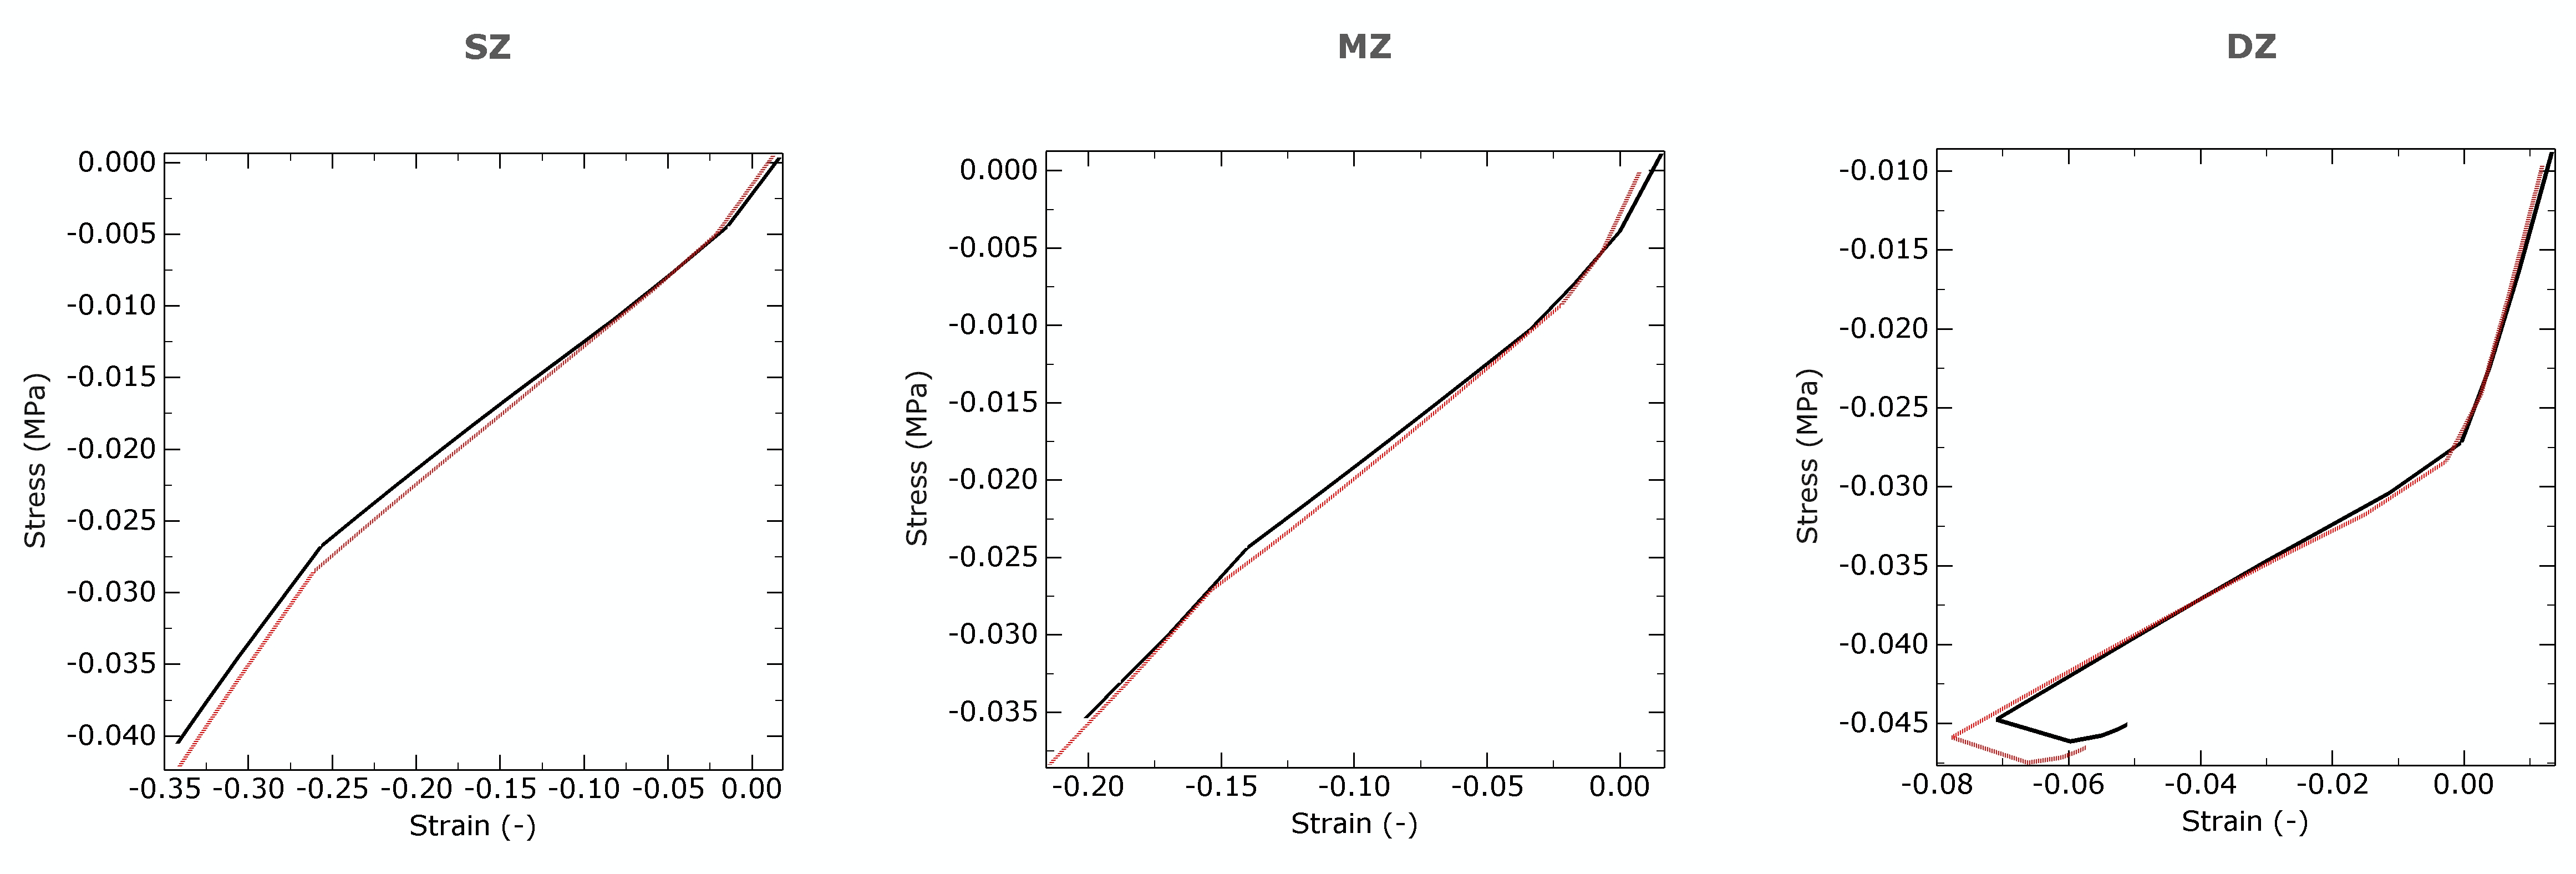
\includegraphics[width=\textwidth]{img/total_stress_strain.jpg}
\caption{Total stress vs strain plots from numerical simulations of unconfined compression experiments with (black curves) and without (red curves) \ac{mo} across different cartilage zones.}
\label{fig:total_stress_strain}
\end{figure}

\paragraph{Joint-scale pre-stressing test.} As depicted in Fig.~\ref{fig:deformation}, the deformation in the post-pre-stressing equilibrium is determined, revealing that the \ac{sz} undergoes the most substantial deformation (reaching up to the contact points). This phenomenon occurs as this particular zone is neither entirely restricted nor subjected to any external pressure. Consequently, in numerical simulations emphasizing the stress levels in these external zones, the pre-stressing effects might be reasonably omitted. In contrast, the behavior of the deeper layers diverges from this trend.
%
\begin{figure}\centering
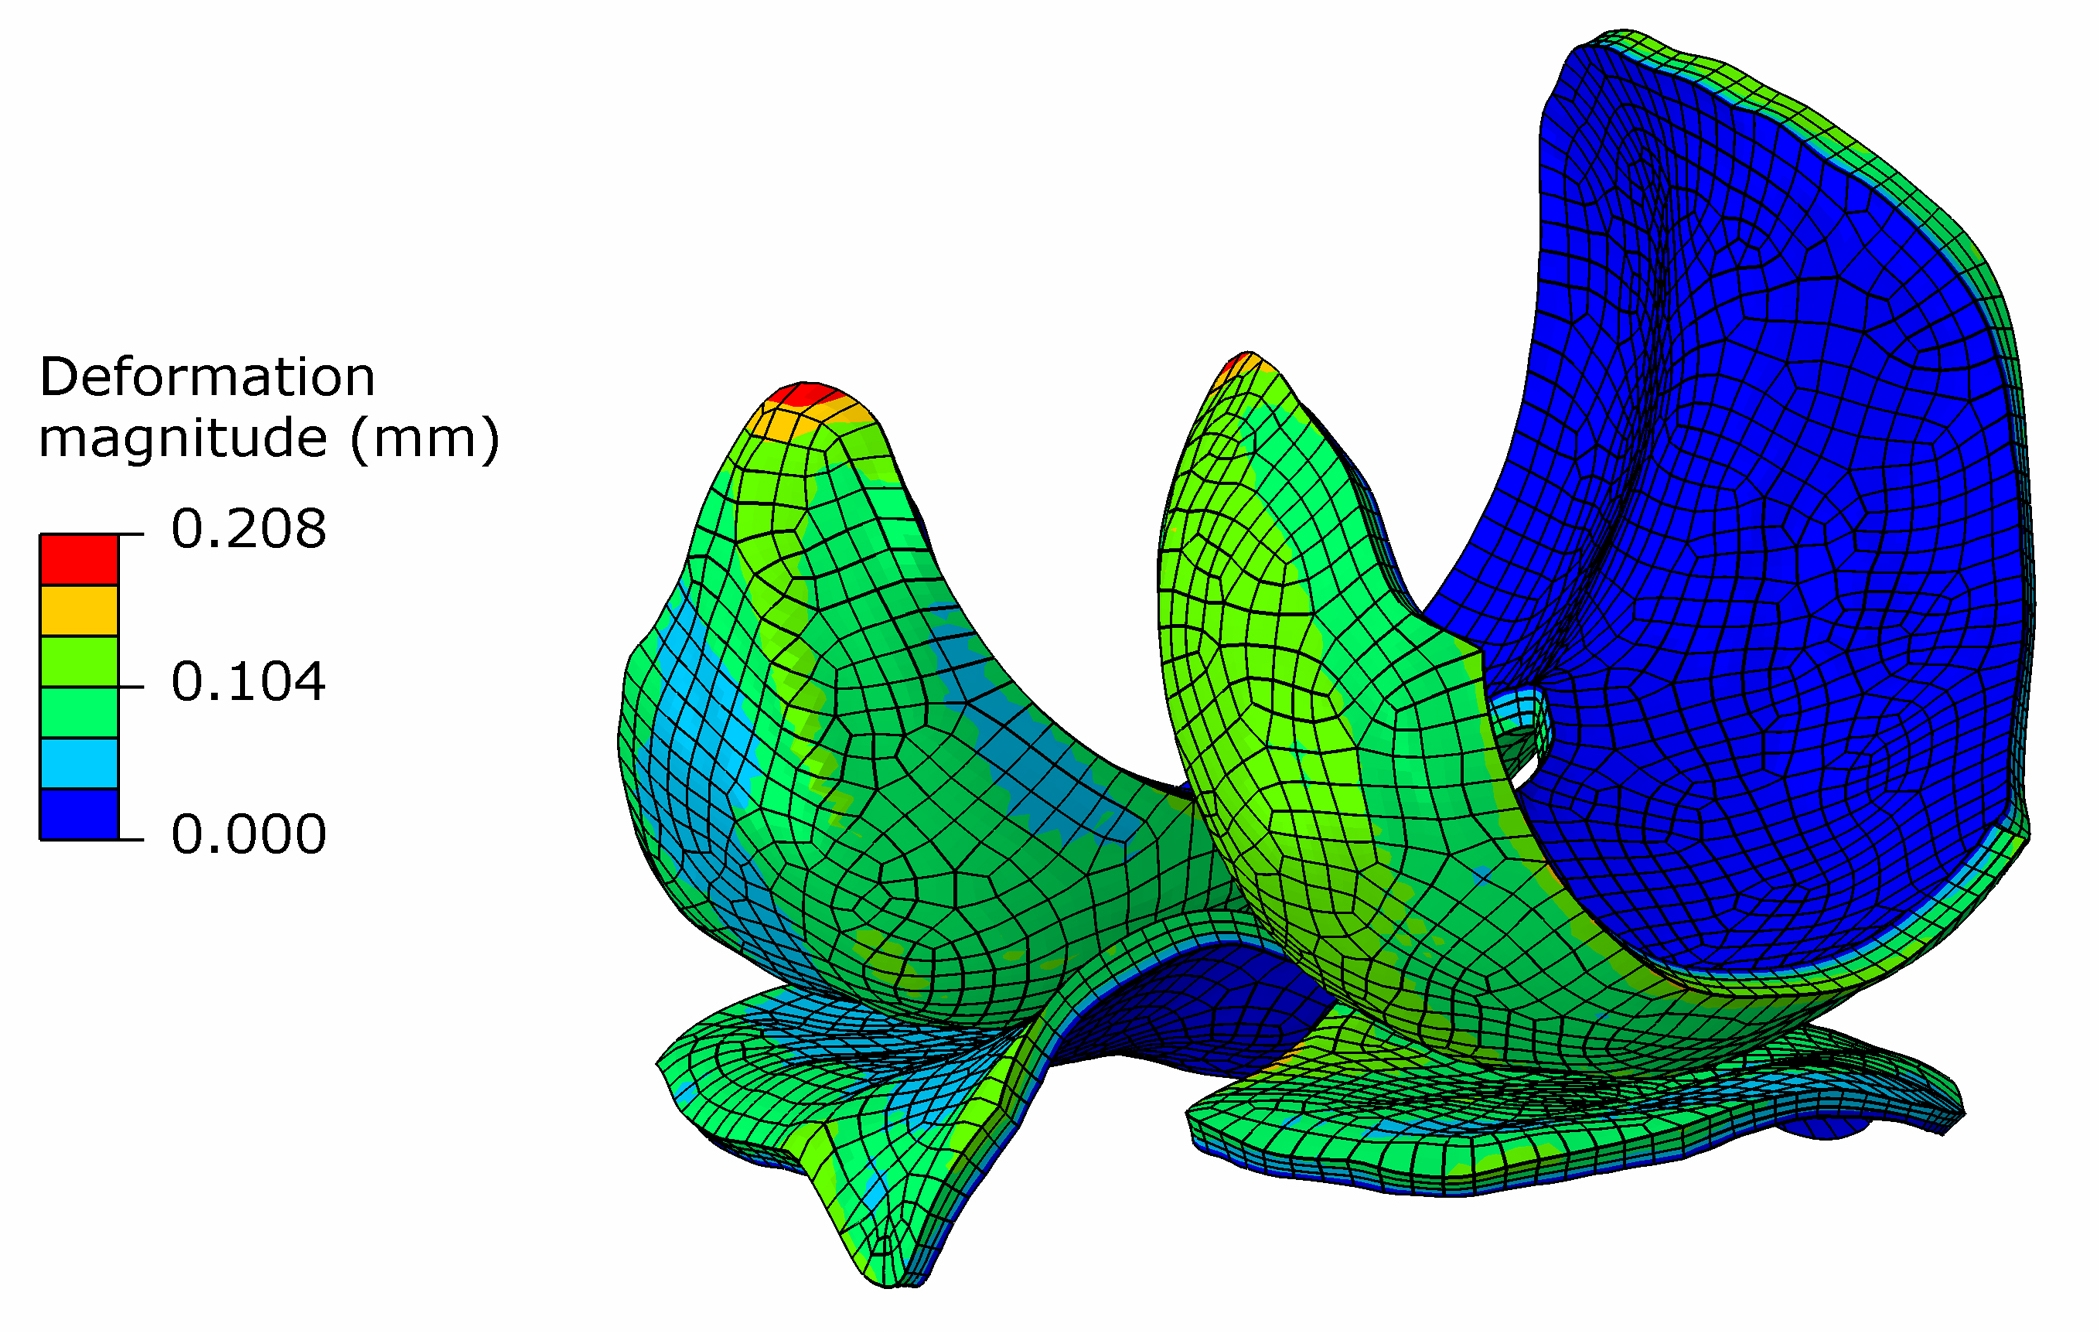
\includegraphics[width=0.55\textwidth]{img/deformation.jpg}
\caption{Contour plot of pre-stressed cartilage deformation.}
\label{fig:deformation}
\end{figure}

The deeper \ac{ac} layers show minimal deformation, attributed to their connection with the subchondral bones. As shown in Fig.~\ref{fig:components}, the deeper layer experiences a fibrillar Mises stress that approximates the overall stress, with values less than $0.2$. These findings are in alignment with stresses reported in existing studies for 10\% strain in compression tests [\cite{sajjadinia2019}], underscoring the major role of pre-stressing with \ac{mo}. Moreover, these stress values can be indirectly validated by considering the pre-stresses obtained from the linear triphasic models [\cite{lai1991,setton1996}], where stress levels fluctuate below 0.4\,MPa based on the direction of the applied load. Compared to them, our large-scale results are also considered reasonable, in light of the different modeling assumptions.
%
\begin{figure}[b!]\centering
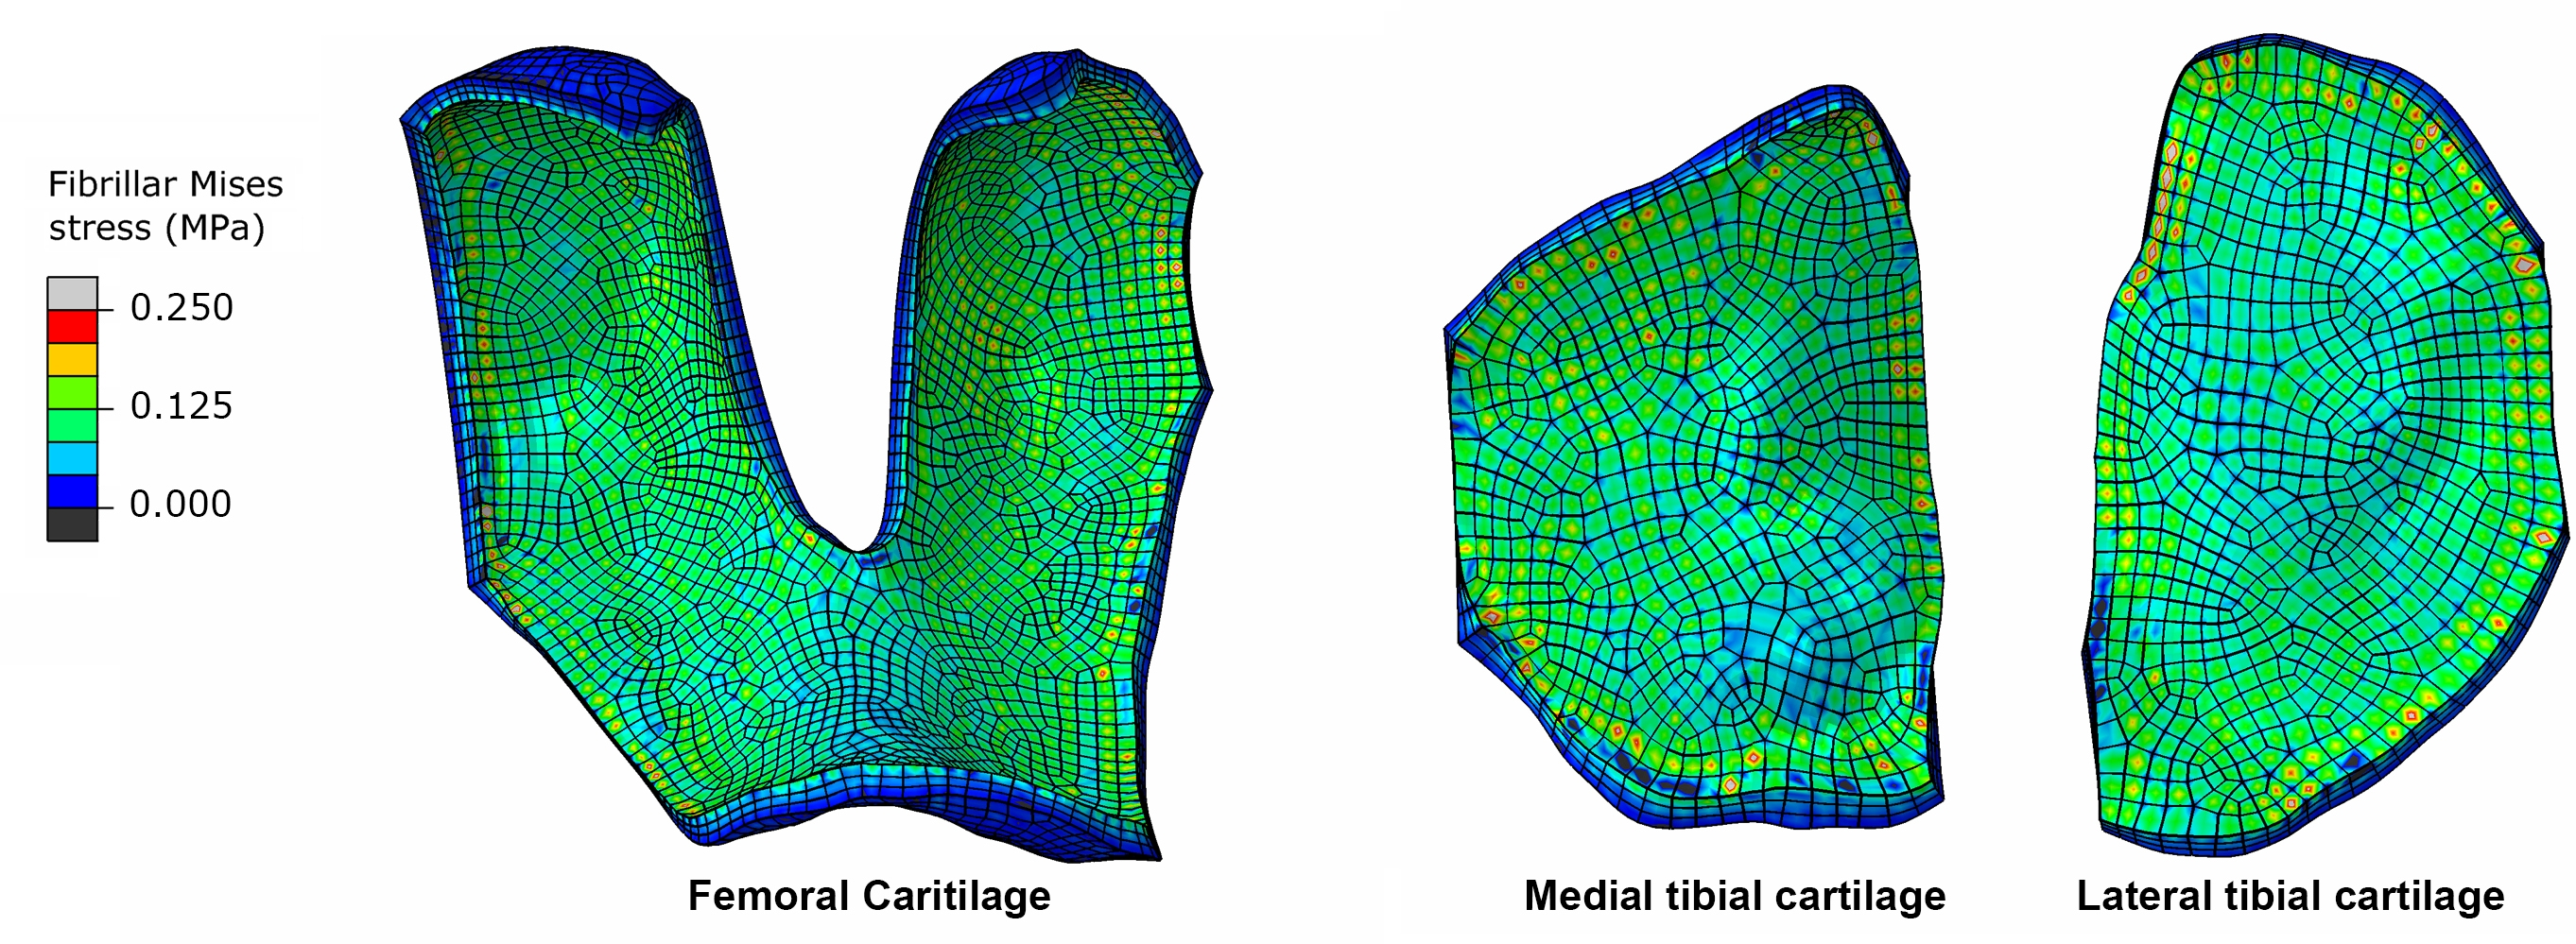
\includegraphics[width=\textwidth]{img/components.jpg}
%\vspace{2.5cm}
\caption{Contour plots of the stresses in the pre-stressed \ac{ac} are presented. Since the \ac{sz} values are negligible, they are not shown here. It is important to note that the constitutive equation for the fibrils is based on the highly discrete orientation of the fibrillar bundles (eq.~\ref{eq-fibril_stress}), leading to non-physiological concentrations of stress in the model. To mitigate this issue, the selection of higher-order elements or the adoption of a denser mesh could have been beneficial. However, given the good agreement of the results with the previous findings, the use of more computationally expensive meshes was deemed unnecessary.}
\label{fig:components}
\end{figure}

\paragraph{Other discussion.} This study acknowledges certain limitations. First, the calibration of the numerical model was performed using a specific type of tensile experiment, similar to the foundational calibration test in the related \ac{psa} work [\cite{wang2018}]. In this way, we approximated the influence of our algorithm on the main constitutive parameters. Second, our \ac{psa} might introduce additional complexity into the \ac{fpbbs}, necessitating the retrieval of deformation gradient values at each integration point. Nonetheless, this is not a significant limitation, as accessing such data is necessary for the \ac{fe} implementation of our multiphasic model. Notably, our \ac{psa} method is comparatively less demanding than the other \acp{psa} that involve element-level manipulations of the \ac{fe} code, for instance, [\cite{pierce2015,weisbecker2014}].

In summary, the \ac{psa} introduced in this study provides a novel and efficient computational approach to be applied to fibril-reinforced and heterogeneous AC models. Our method takes into account the experimentally-observed initial state of both constitutive and geometrical parameters. Several comparative analyses shed light on the importance of such a \ac{psa} in the stress evaluation of pre-stressed AC components. Our work also delves into large-scale pre-stressing, showing that pre-stressing can lead to considerable deformation and initial stress distribution. This highlights the criticality of accurately determining the stress-free state. Therefore, this efficient \ac{psa}, to be used in the next chapter, is deemed highly relevant in multiphasic AC research, especially in scenarios where osmotic pressure is a pivotal consideration.


\chapter{Efficient Surrogate Modeling with Hybrid Multi-Fidelity Learning}\label{ch4}

The iterative nature of numerical modeling in cartilage biomechanics, whether with or without additional complexities such as \ac{psa}, renders most of these methods inefficient. As explained in Chapter~\ref{ch2}, one solution is to use \ac{ml}-based surrogates. This chapter introduces a novel surrogate modeling technique using an \ac{hml} method that combines reduced-order numerical analysis with traditional supervised \ac{ml}. This method aims to train surrogates of soft tissues like cartilage with a limited number of training samples, as generating \ac{hf} numerical data with multi-physics models can be very time-consuming. The feasibility of this technique is empirically evaluated and compared with purely data-driven baselines (including \acp{gnn} and \acp{ffnn}) across diverse scales.

\section{Related Work}

\paragraph{Data-driven surrogates.} The application of surrogate models proved to be an efficient replacement for computationally demanding numerical models [\cite{cai2021,liu2019,martinez2017}]. Surrogate modeling finds extensive use in biomechanical studies. Examples include deformation analysis of breast and liver employing tree-based algorithms [\cite{martin-guerrero2016}], prostate modeling using \acp{ffnn} [\cite{jahya2013}], and many more. In cartilage modeling, \acp{ffnn} have been trained using data from simplified numerical models, e.g., the surrogate of the elastic model in [\cite{paiva2012}]. Another study incorporated biphasic formulations into a small-scale cartilage model surrogate but neglected the tissue's swelling [\cite{arbabi2016a}]. Further advancements were made by employing multi-physics models in surrogate training, albeit with a significant sample size of $10\,000$ [\cite{arbabi2016b}]. However, despite their potential, surrogate models are not widely utilized due to the requirement of generating costly numerical samples [\cite{frank2020}].

Utilizing optimized computational code, e.g., through \ac{gpu} acceleration, can mitigate the above-mentioned issue [\cite{johnsen2015}], although it might demand specific software and hardware not always available [\cite{marinkovic2019}]. Another remedy is to create the surrogate with minimal data under certain conditions, such as reduced simulation scales [\cite{faisal2023}]. Nonetheless, complex multi-physics simulations might still be too costly to be implemented. If the main goal of integrating \ac{ml} is to increase efficiency, then the models should be trained with as few samples as possible. This is the main reason behind the underutilization of such AI-enhanced modeling.

\paragraph{Data-efficient learning.} The challenge of small training sets in surrogate modeling can be effectively tackled by integrating physical laws and domain-specific insights into the training methodology. Such integration, as shown by \cite{kashinath2021,linka2021,hoerig2020}, has been shown to enhance performance even with limited data. These methods, despite their evident success, are still evolving and require meticulous design and complex coding. Often, they introduce new constraints to the training, such as loss function penalization in standard learning algorithms. Challenges particularly arise in dealing with multi-physics scenarios and discontinuities in mechanical models, as discussed in \cite{coutinho2023,cai2021b,karniadakis2021,fuks2020}.

Another approach to managing limited data involves simplifying the numerical model to focus on key information, thus reducing the number of necessary parameters. This method is exemplified in studies by \cite{pellicer-valero2020,niroomandi2012}. The efficiency gains from such \ac{mor} methods have sparked interest in various domains, e.g., the virtual reality applications in surgical simulations [\cite{cueto2014}]. However, these methods also present challenges in implementation, as noted in the \cite{lauzeral2019} study. Considering this, multi-fidelity methods in the \ac{mor} offer an alternative, potentially implemented with non-destructive methods (without directly affecting the numerical solvers). These techniques have shown promising results across different fields, implemented with diverse \ac{ml} methods [\cite{ahn2022,zhang2022,cheng2021,yang2019}].

A prevalent strategy in multi-fidelity \ac{mor}-based surrogate modeling involves using an \ac{lf} model in conjunction with an \ac{ml} model to enhance the \ac{lf} output accuracy, as detailed by \cite{peherstorfer2018}. Such models have found applications in diverse fields using various \ac{lf} modeling implementations [\cite{zhang2021,zhou2017}]. However, to our knowledge, no implementation has been done using \ac{lf} modeling for multi-physics soft tissue models, like cartilage, as proposed in our study. The proposed approach utilizes an \ac{lf} numerical part that simplifies the multi-physics equations, focusing on the tissue's approximate behavior. The accuracy of the \ac{lf} outcomes is then enhanced through an \ac{ml} model to match the \ac{hf} model's precision with non-destructive \ac{hml} implementation.

\section{Methodology}

\subsection{Efficient Hybrid Learning}

In the following of this chapter, we use the term \ac{ml} to primarily denote the conventional \ac{ml}-based predictive models, except when specified otherwise, as illustrated in Fig.~\ref{fig:ml_system}(a). In a standard supervised learning approach, an \ac{fe} model generates various informative training samples at distinct analysis points using a comprehensive physical model. These \ac{hf} outcomes serve as the target \ac{ml} dataset, while the input features may include various physical parameters, such as boundary conditions and material properties.
%
\begin{figure}[H]\centering
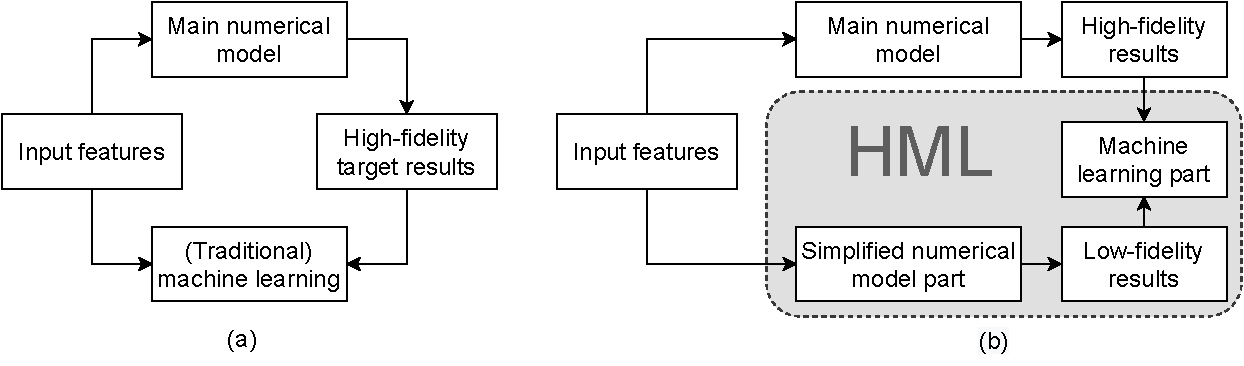
\includegraphics[width=\textwidth]{img/ML.pdf}
\caption{Illustration of a standard machine learning surrogate model (a) and its integration in a hybrid machine learning (HML) framework, as connected with a simplified \ac{fe} model sequentially (b).
\label{fig:ml_system}}
\end{figure}

In the proposed \ac{hml} approach, we initiate with an \ac{lf} model derived by simplifying the \ac{hf} equations. This computationally efficient model provides a basic estimate of the system's behavior and precedes the \ac{ml} component, which aims to refine these initial predictions to match the accuracy of the \ac{hf} model. In essence, the \ac{ml} component's input features are derived from the outputs of the \ac{lf} model, as depicted in Fig.~\ref{fig:ml_system}(b).

While this methodology offers considerable flexibility in choosing the \ac{lf} model, it necessitates the creation of two distinct training datasets using varied computational techniques. Nevertheless, this may not be a significant limitation, as the \ac{lf} model is just the simplified and more efficient version of the main \ac{hf} model. Our empirical analysis, explained in the next section, indicates that this approach may also require fewer training samples overall to achieve comparable accuracy and potentially offers faster training convergence; thereby considerably mitigating the high computational demands typically associated with training and data generation.

For instance, a complex \ac{hf} physical model might be defined by using biphasic equations. In contrast, a corresponding \ac{lf} model is the same \ac{fe} model but could be represented by simpler monophasic equations, which, while not capturing the intricacies of each phase, approximates the overall system response. Depending on the specific physical problem, various combinations of equations can be employed. Accordingly, in the following, we explore two different selections of \ac{lf} modeling to test the applicability of this method.

\subsection{Simulation Tests}

We develop two computational physics problems for generating datasets, via \ac{fe} modeling. These problems replicate standard \ac{2d} and \ac{3d} tests on artificial soft tissues, which are commonly employed in repetitive biomechanical simulations. The mathematical formulations and their computational implementations are elaborated in Chapters~\ref{ch2} and \ref{ch3}.

\paragraph{2D problem.} This involves a small-scale problem where a soft biological material is subjected to 2D load testing. This is depicted in Fig.~\ref{fig:2d_model} (left). We model a rectangular specimen of dimensions $0.3 \times 1.0$\,mm$^2$ using a hybrid \ac{fe} model. A porous hyperelastic material model is used (as per eq.~\ref{eq-non_fibrillar} with $\emptyset_0^{\rm S}=0.15$), along with osmotic pre-stress (see eq.~\ref{eq-osmotic} with $\alpha_2 = 3.22$). Here, $\alpha_1$ represents the adjustable input parameter in our surrogate model. We deliberately omit fibrillar and fluid constituents for computational efficiency. Obviously, our \ac{psa} is essential for initializing the numerical experiments, while the \ac{lf} model is simplified by excluding the pre-stressing feature.
%
\begin{figure}\centering
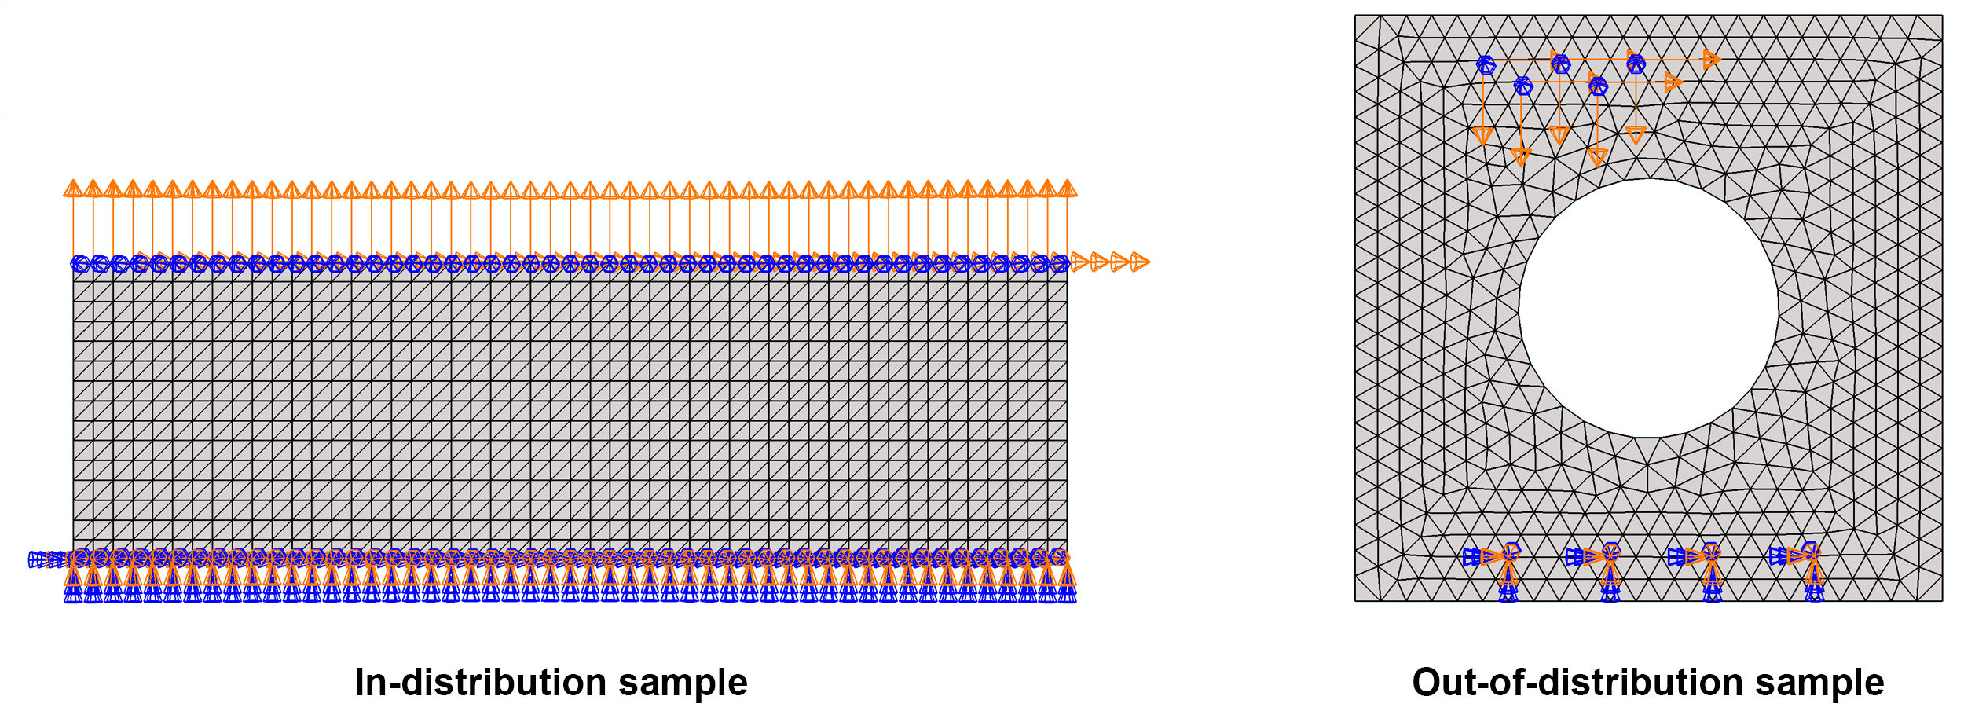
\includegraphics[width=\linewidth]{2d_model.pdf}
\caption{Illustration of various small-scale computational samples for surrogate modeling.\label{fig:2d_model}}
\end{figure}

To assess the model's capacity to handle out-of-distribution scenarios, we also evaluate a different \ac{2d} setup; see Fig.~\ref{fig:2d_model} (right). This setup involves different load applications and geometry, specifically a $0.9 \times 0.9$\,mm$^2$ specimen with a central circular hole of $0.2$\,mm in radius. In both simulations, we fix the bottom surface of the tissue and apply displacement conditions at the top. For the mesh, the linear and plane strain triangular elements are used.

\paragraph{3D problem.} Our large-scale simulations apply the tibiofemoral model introduced in Chapter~\ref{ch3}, but they utilize different multi-physics equations. This test aims to analyze the influence of varying body weights on one of the cartilage substructures (refer to Fig~\ref{fig:3d_model}). We implement a hyperelastic equation for \ac{lf} modeling, based on eq.~\ref{eq-hyperelastic}, where $C_{10} = 2.48$\,MPa and $D_1 = 0.59$\,MPa$^{-1}$, whereas the \ac{hf} model adds also inviscid water component to the constitutive equations.
%
\begin{figure}\centering
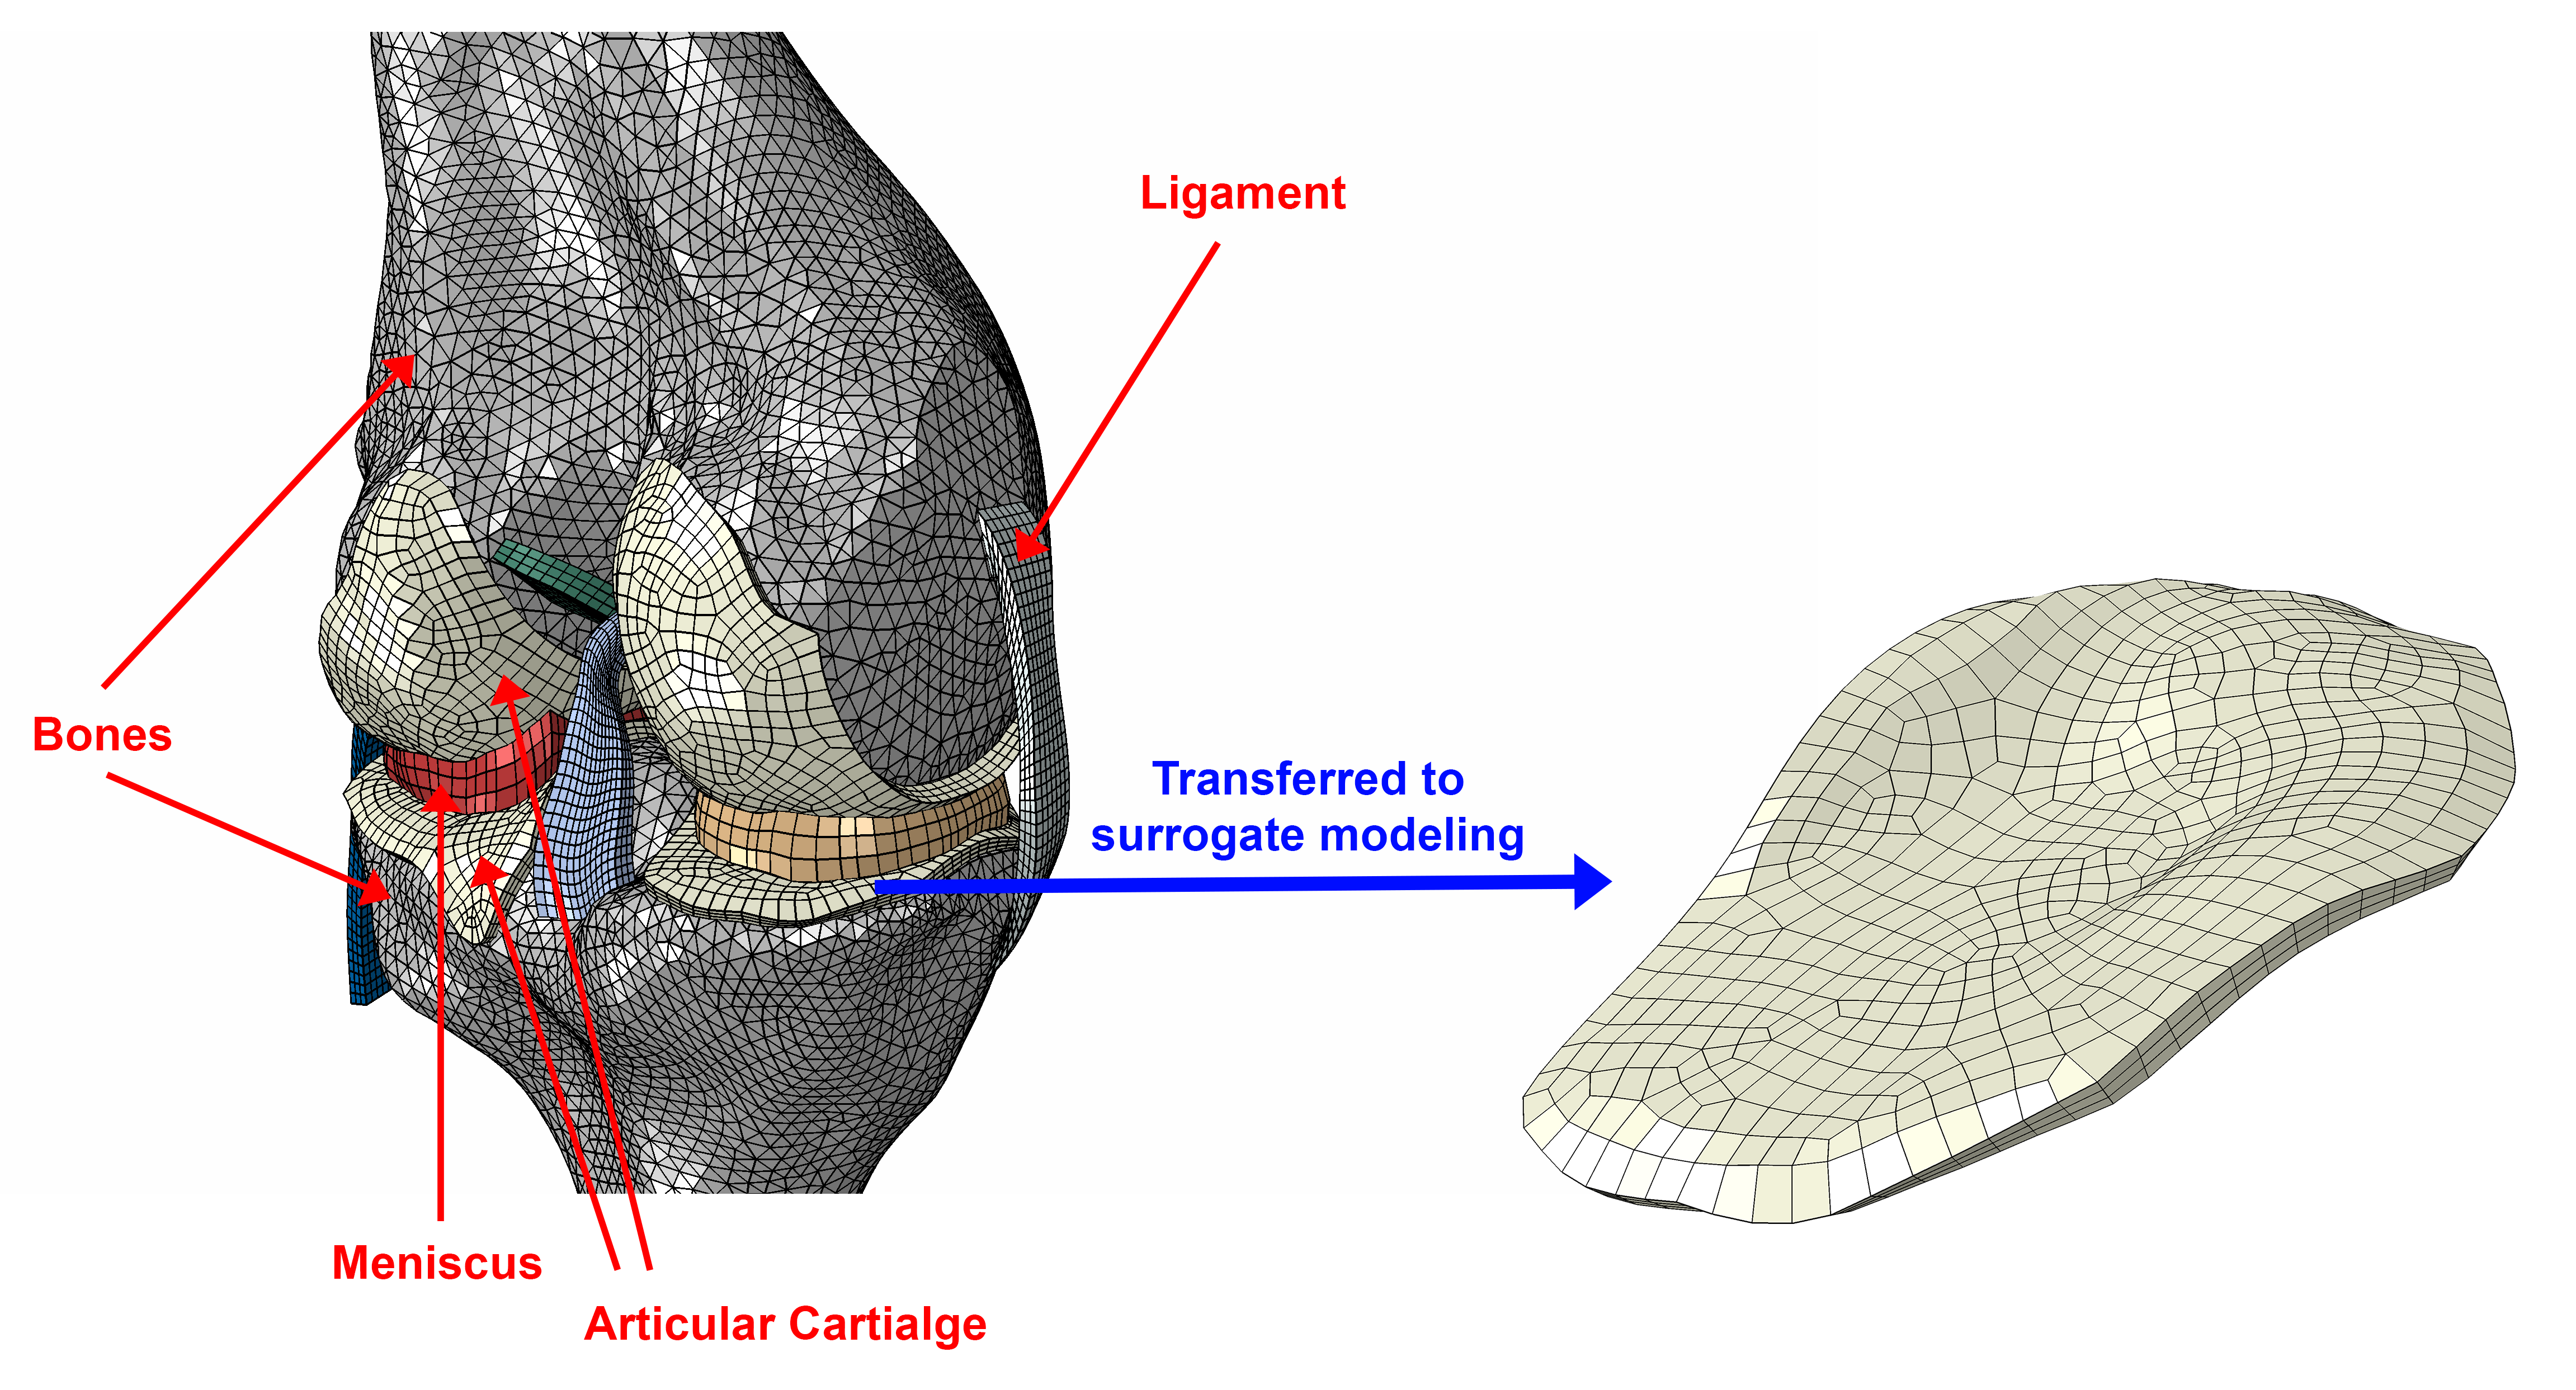
\includegraphics[width=\linewidth]{3D_model.png}
\caption{Numerical mesh of the large-scale problem used for creating surrogate models.\label{fig:3d_model}}
\end{figure}

In the biphasic model for \ac{hf} simulations, we use first-order elements to accelerate data generation. The permeability parameters are derived from existing literature on the cartilage \ac{mz} [\cite{sajjadinia2019,stender2016}]. While the fluid is allowed to move freely across the cartilage surfaces, the weight is applied uniformly across the femur, with the fixed tibia and no flexion-extension motion.

\paragraph{Datasets and evaluation.} For the datasets of the \ac{2d} models, $20$ representative samples are generated. These samples are derived from a uniform distribution ($U$), encompassing two displacement-based boundary conditions within $U$($-0.1$\,mm, $0.1$\,mm), a constitutive variable $\alpha_1$ ranging from $U$($0.005$, $0.010$\,MPa), and a one-hot vector to distinguish the fixed nodes with the others. Minor noise is introduced at each node to enhance model generalizability. Thus, the nodal coordinates are additional input features, while the introduced noise impacts the initial conditions and influences all subsequent model outputs.

The outputs from both \ac{lf} and \ac{hf} simulations consist of computed nodal deformation and total stress values. For model validation, we generate $10$ additional in-distribution samples with varied inputs. Our test set, which also comprises $10$ samples, employs the out-of-distribution \ac{fe} model, testing the model's adaptability to unseen conditions.

For the large-scale surrogate model, we create $100$ samples. Inputs for the \ac{hf} model include a range of the weight from $U$($-900$\,N, $-400$\,N). Outputs cover determined normal stress and strain at each node, whereas the \ac{lf} outputs focus on nodal deformation. We randomly distribute these samples across training, validation, and testing subsets, with the validation set sized at a third of the training set. The exact count of training samples is noted in the results, emphasizing the scarcity of such data.

Notably, the range of \ac{2d} problem results generally falls under a similar range between $10^{-1}$ and $10^{-3}$, considering their units and absolute values. Thus, we employ an unscaled \ac{mse} metric for all node outputs in all the evaluation samples. This allows simple comparison between different training conditions. Conversely, for the \ac{3d} models, due to the vast difference in input-output scales, target feature normalization based on training samples is necessary. Although this normalization facilitates comparison across different outputs, the use of \acp{mse} can sometimes be deceptive, as it may average out anomalous nodes with scaled outputs. To address this, we use the \ac{pmse} metric, averaging these scaled values individually for each node.

\paragraph{Training settings.} Our approach adapts the previously used MeshGraphNets method [\cite{pfaff2021}] for our specific \ac{2d} surrogate model needs. The original framework, based on a \ac{gnn}, incorporates a series of \acp{ffnn} organized into encoder, processor, and decoder modules [\cite{sanchez2020,battaglia2018}]. This architecture facilitates local learning at each node and connected edges, enhancing spatial equivariance through bidirectional edge sets. The core model initially encodes node and edge features into latent representations, which are then sequentially processed by message-passing blocks. While the residual connections further augment the latent vectors, enhancing the model's convergence [\cite{sanchez2020}], the final latent representation is decoded into the surrogate outputs.

We diverged from the standard MeshGraphNets implementation by omitting domain-specific configurations, particularly the separate edge types, as they were irrelevant for our \ac{2d} tests lacking mechanical contact. Also, instead of the original noise strategy, we use our aforementioned noise generation method. We also revised the preprocessors and evaluation algorithms of the trained model, tailoring them for static system simulations of this study that focus solely on end conditions as outputs.

To develop \ac{2d} model $1$, we employ a training method that accommodates various input sample sizes, utilizing an $L_2$ loss function for nodal results. The training involves a maximum of $1\,000$ steps, with a learning rate of $10^{-3}$ and the first ($100$) steps dedicated to initializing the online normalizer [\cite{sanchez2020}]. The model's \acp{ffnn} components comprise three hidden layers, and we included three message-passing blocks (containing such \acp{ffnn}) with a latent size of $40$.  This size is also the same as the encoder output size and the decoder input size.

Furthermore, the edge sets are constructed from relative nodal distances and their euclidean norms, with the encoder's input shape set to size $3$. In the hybrid model, the node set is made by the nodal outputs, leading to an encoder's input size of $6$ and a decoder's output size of $6$. The batch size is set to the total node count of each sample (i.e., $816$), and the rest of the hyperparameters are identical to the original study.

Our study also includes an empirical comparison of \ac{3d} models built using standard \acp{ffnn}. We optimized these models for rapid convergence by maintaining a minimal neuron and layer count. After extensive manual tuning of hyperparameters, \ac{3d} model $1$ was configured with four hidden layers, each containing $940$ neurons equipped with the ReLU activation functions and subsequent normalization layers. The output dimension matches the size of the total nodal results of each one of the \ac{hf} samples (i.e., $94\,032$). The input dimension of the \ac{ml} surrogate is $1$, while for the \ac{hml} model's \ac{ml} component, it equals the total nodal results of each of the \ac{lf} samples (i.e., $8\,364$). Training is conducted on a limited number of samples with a $10^{-4}$ learning rate. For the other settings, we adhere to the default library settings.

While we also open-sourced\footnote{\href{https://github.com/shayansss/hml}{https://github.com/shayansss/hml}.} all the code for further details, in the following section, we will detail additional models, their configuration, and training to assess the impact of hyperparameters and training sample sizes.

\section{Results and Discussion}
%
Empirical tests were conducted using various \ac{lf} and \ac{hf} computational models on a regular computer. The efficiency gains are illustrated in Fig.~\ref{fig:runtime-comparison} using a violin plot [\cite{hintze1998}]. These gains underscore the practicality of employing LF models over HF ones. Variations in the loading rate applied in the 3D simulations led to a broader range of computation times. It is important to note that in real-world scenarios, this disparity might be more pronounced, given that the HF simulations were modified in this study to expedite the process of surrogate model development.
%
\begin{figure}\centering
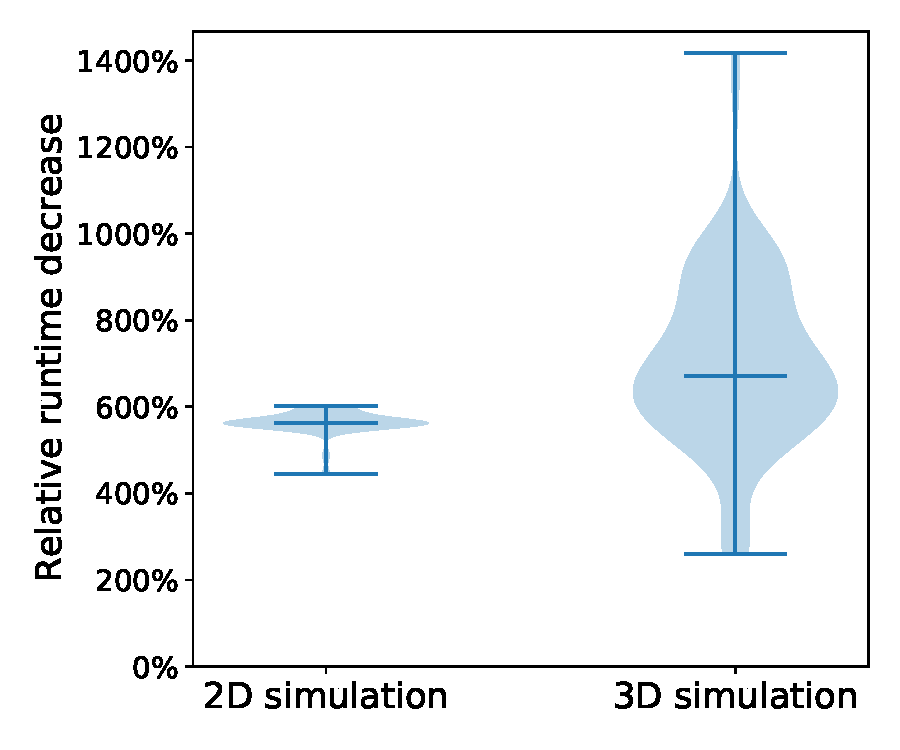
\includegraphics[trim={0cm 0.5cm 0cm 0cm},clip,width=7cm]{comparison.pdf}
\caption{Representation of the relative decrease in runtime for HF simulations compared to LF simulations. This data is obtained by calculating the ratio of the runtime reductions to the runtimes of the LF simulations.\label{fig:runtime-comparison}}
\end{figure}

In our analysis, the runtime of \ac{ml} inference was not considered as it occurred in real time, and the majority of computational expenses were attributed to the generation of numerical data. In the following, we provide a comparative analysis of \ac{hml} and \ac{ml} methods across different simulation scenarios, highlighting the efficacy of HML models when using a limited number of HF samples. Conducting a couple of independent multi-physics tests with varying surrogate modeling assumptions enabled an effective assessment of model performance under diverse training settings.

\paragraph{2D simulation.} The evaluation of \acp{mse} for both in- and out-of-distribution sets, in the context of \ac{2d} simulations, is depicted in Fig.~\ref{fig:tuner}. We deliberately use small datasets, as it is usually the case for soft material surrogate modeling [\cite{liu2019}]. The \ac{hml} frameworks demonstrate superior performance compared to \ac{ml} models. The errors in most cases for \ac{hml} models are at or below $10^{-4}$, with a notable exception being the error for the hybrid surrogate trained with four samples. However, this error is still lower than any error observed in the \ac{ml} models. Further experiments were conducted using a different setting (model $2$), characterized by less efficient, yet increased learnable parameters, as it incorporates three additional message-passing phases as the principal hyperparameter [\cite{pfaff2021}]. Even with a learning rate set to $10^{-4}$ and training steps increased by a factor of eight, the results remained consistent, underscoring the precision and generalizability of the \ac{hml} models.

\begin{figure}[b!]\centering
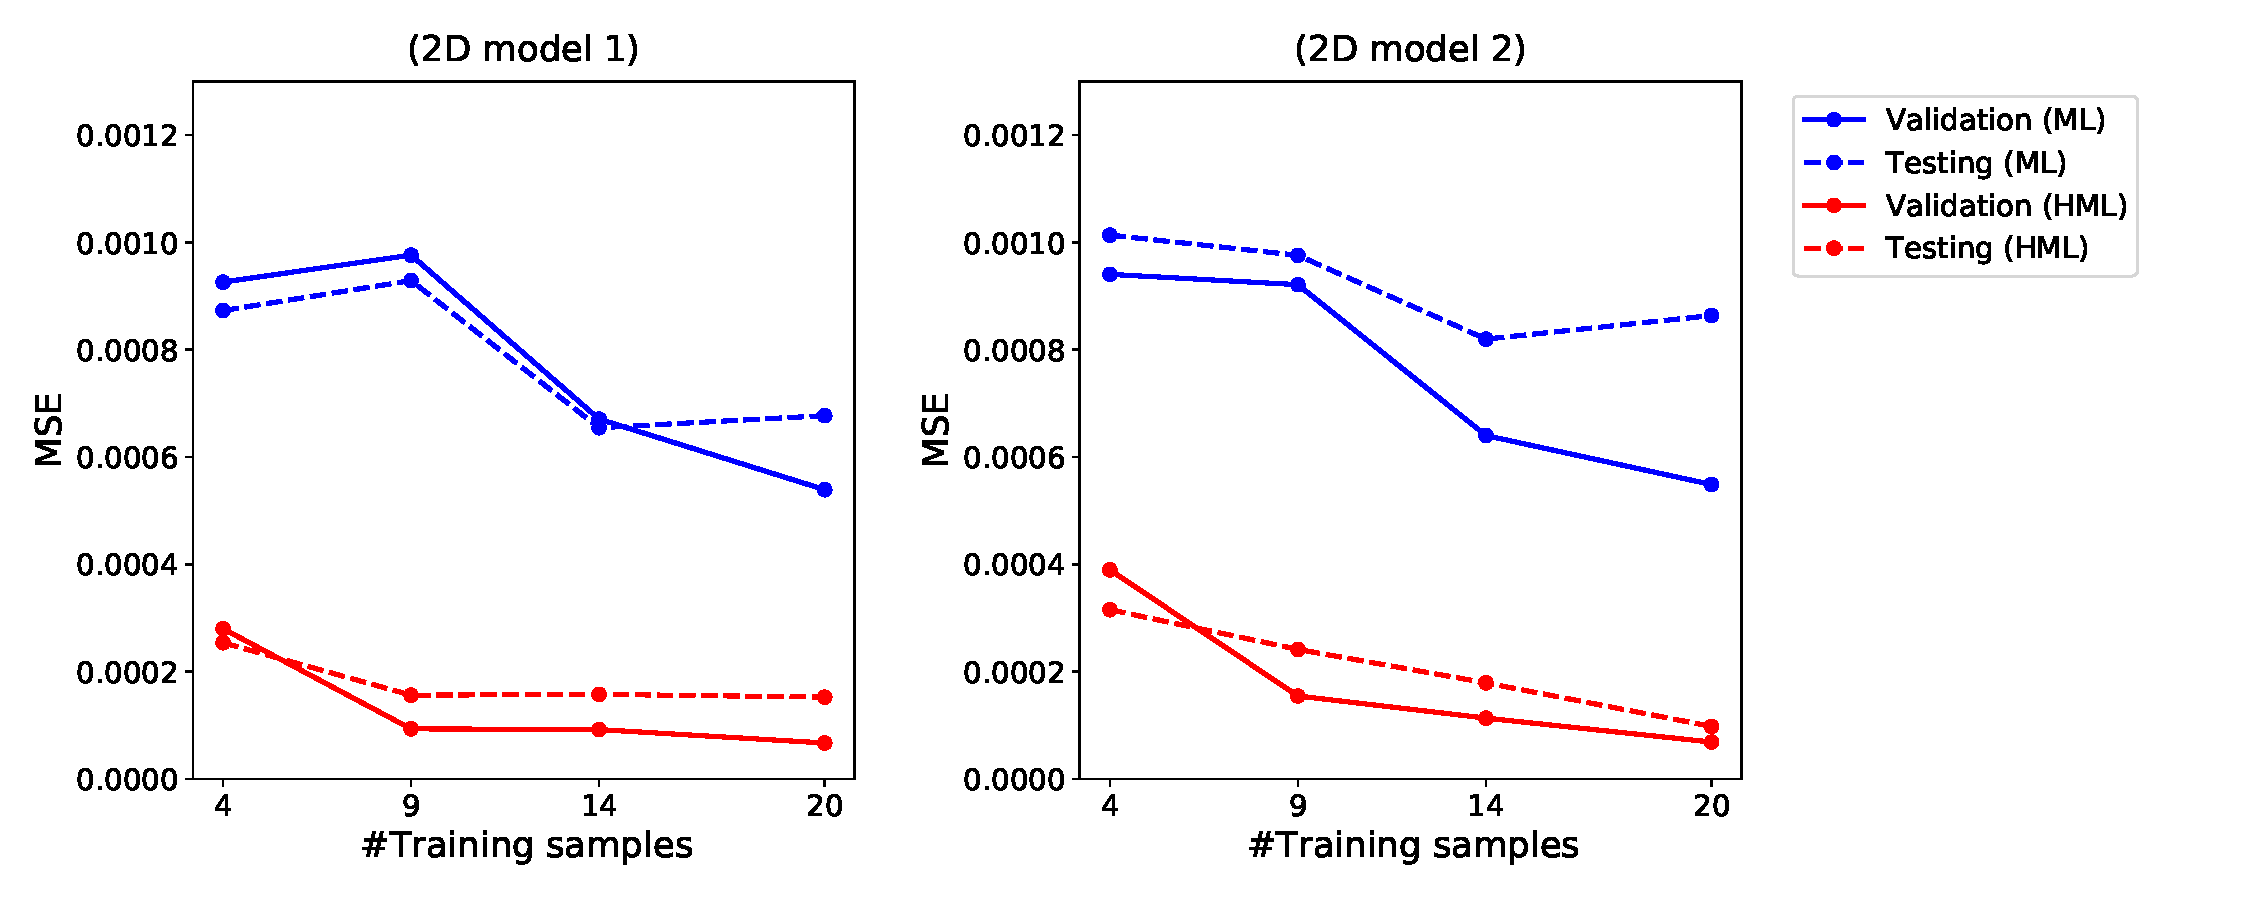
\includegraphics[trim={0.5cm 0.5cm 1.5cm 0cm},clip,width=\linewidth]{2d.pdf}
\caption{Assessment of the trained models with different numbers of training samples in 2D tests. \label{fig:tuner}}
\end{figure}

Furthermore, the \ac{hml} model's methodology, mapping input features into a new representation for subsequent data-driven analysis, bears resemblance to feature-based transfer learning. In such transfer learning, source features are transformed to facilitate knowledge transfer from one domain to another [\cite{zhuang2021}]. Unlike common data-driven models, which employ feature transformation strategies [\cite{pan2011,dai2007,prague2007}], the \ac{hml} model uses a physics-based algorithm, the \ac{lf} model, for transforming input data into more informative representations. This approach mirrors the transfer learning concept and elucidates the enhanced performance of the \ac{hml} model under the constraints of efficient training settings and limited training data availability.

An additional aspect of our study involved assessing how the accuracy of \ac{lf} modeling impacts the performance of \ac{hml} modeling. For this, we replicated the \ac{2d} tests using the same \ac{hml}, but substituting \ac{lf} results with \ac{hf} outcomes. As presented in Table~\ref{table:2d}, this modification yielded errors comparable to the original \ac{lf} inputs, indicating that the model, already adeptly trained with \ac{lf} data, managed to perform effectively despite the inherent stochasticity of the training process. This observation suggests that even potential inaccuracies in \ac{lf} modeling, as also reported in Chapter~\ref{ch3} and other \ac{psa} studies [\cite{bols2013,wang2018}], do not hinder its ability to generate an informative representation for the downstream \ac{ml} part.
%
\begin{table}[H]
\centering
\caption{Recorded MSEs ($\times 10^{-3}$) on validation/testing sets in 2D modeling.}
\begin{tabular}{lccccc}
\toprule
\textbf{Surrogate model} & \multicolumn{4}{c}{\textbf{Training set size}} \\\cmidrule{2-5}
 &    4 &   9 &   14 &    20 \\
\midrule
ML 1 &                     0.93 / 0.87 &  0.98 / 0.93 &  0.67 / 0.65 &  0.54 / 0.68 \\
HML 1 &                               0.28 / 0.25 &  0.09 / 0.16 &  0.09 / 0.16 &  0.07 / 0.15 \\
HML 1 (with HF inputs) &   0.33 / 0.26 &  0.10 / 0.16 &  0.07 / 0.13 &  0.06 / 0.12 \\
ML 2 &                     0.94 / 1.01 & 0.92 / 0.98 &  0.64 / 0.82 &  0.55 / 0.86 \\      
HML 2 &                               0.39 / 0.32 &  0.15 / 0.24 &  0.11 / 0.18 &  0.07 / 0.10 \\      
HML 2 (with HF inputs) &   0.32 / 0.35 &  0.09 / 0.16 &  0.16 / 0.17 &  0.06 / 0.12 \\      
\bottomrule
\end{tabular}
\label{table:2d}
\end{table}


\paragraph{3D simulation.}  As depicted in Fig~\ref{fig:3D}, the $l_2$ loss values captured during the training phase are compared. The \ac{3d} model $1$, incorporating the \ac{hml} framework, demonstrated superior performance over its \ac{ml} counterpart. Another variant, \ac{3d} model $2$, adhered to an identical sample regimen (comprising three training and one validation sample) yet employed the ELU activation function. The outcomes of this model variation were not markedly different, with the \ac{hml} surrogate still having a negligible error. A critical observation here is the rapid and efficient training process, as it only used $100$ epochs.
%
\begin{figure}[t!]\centering
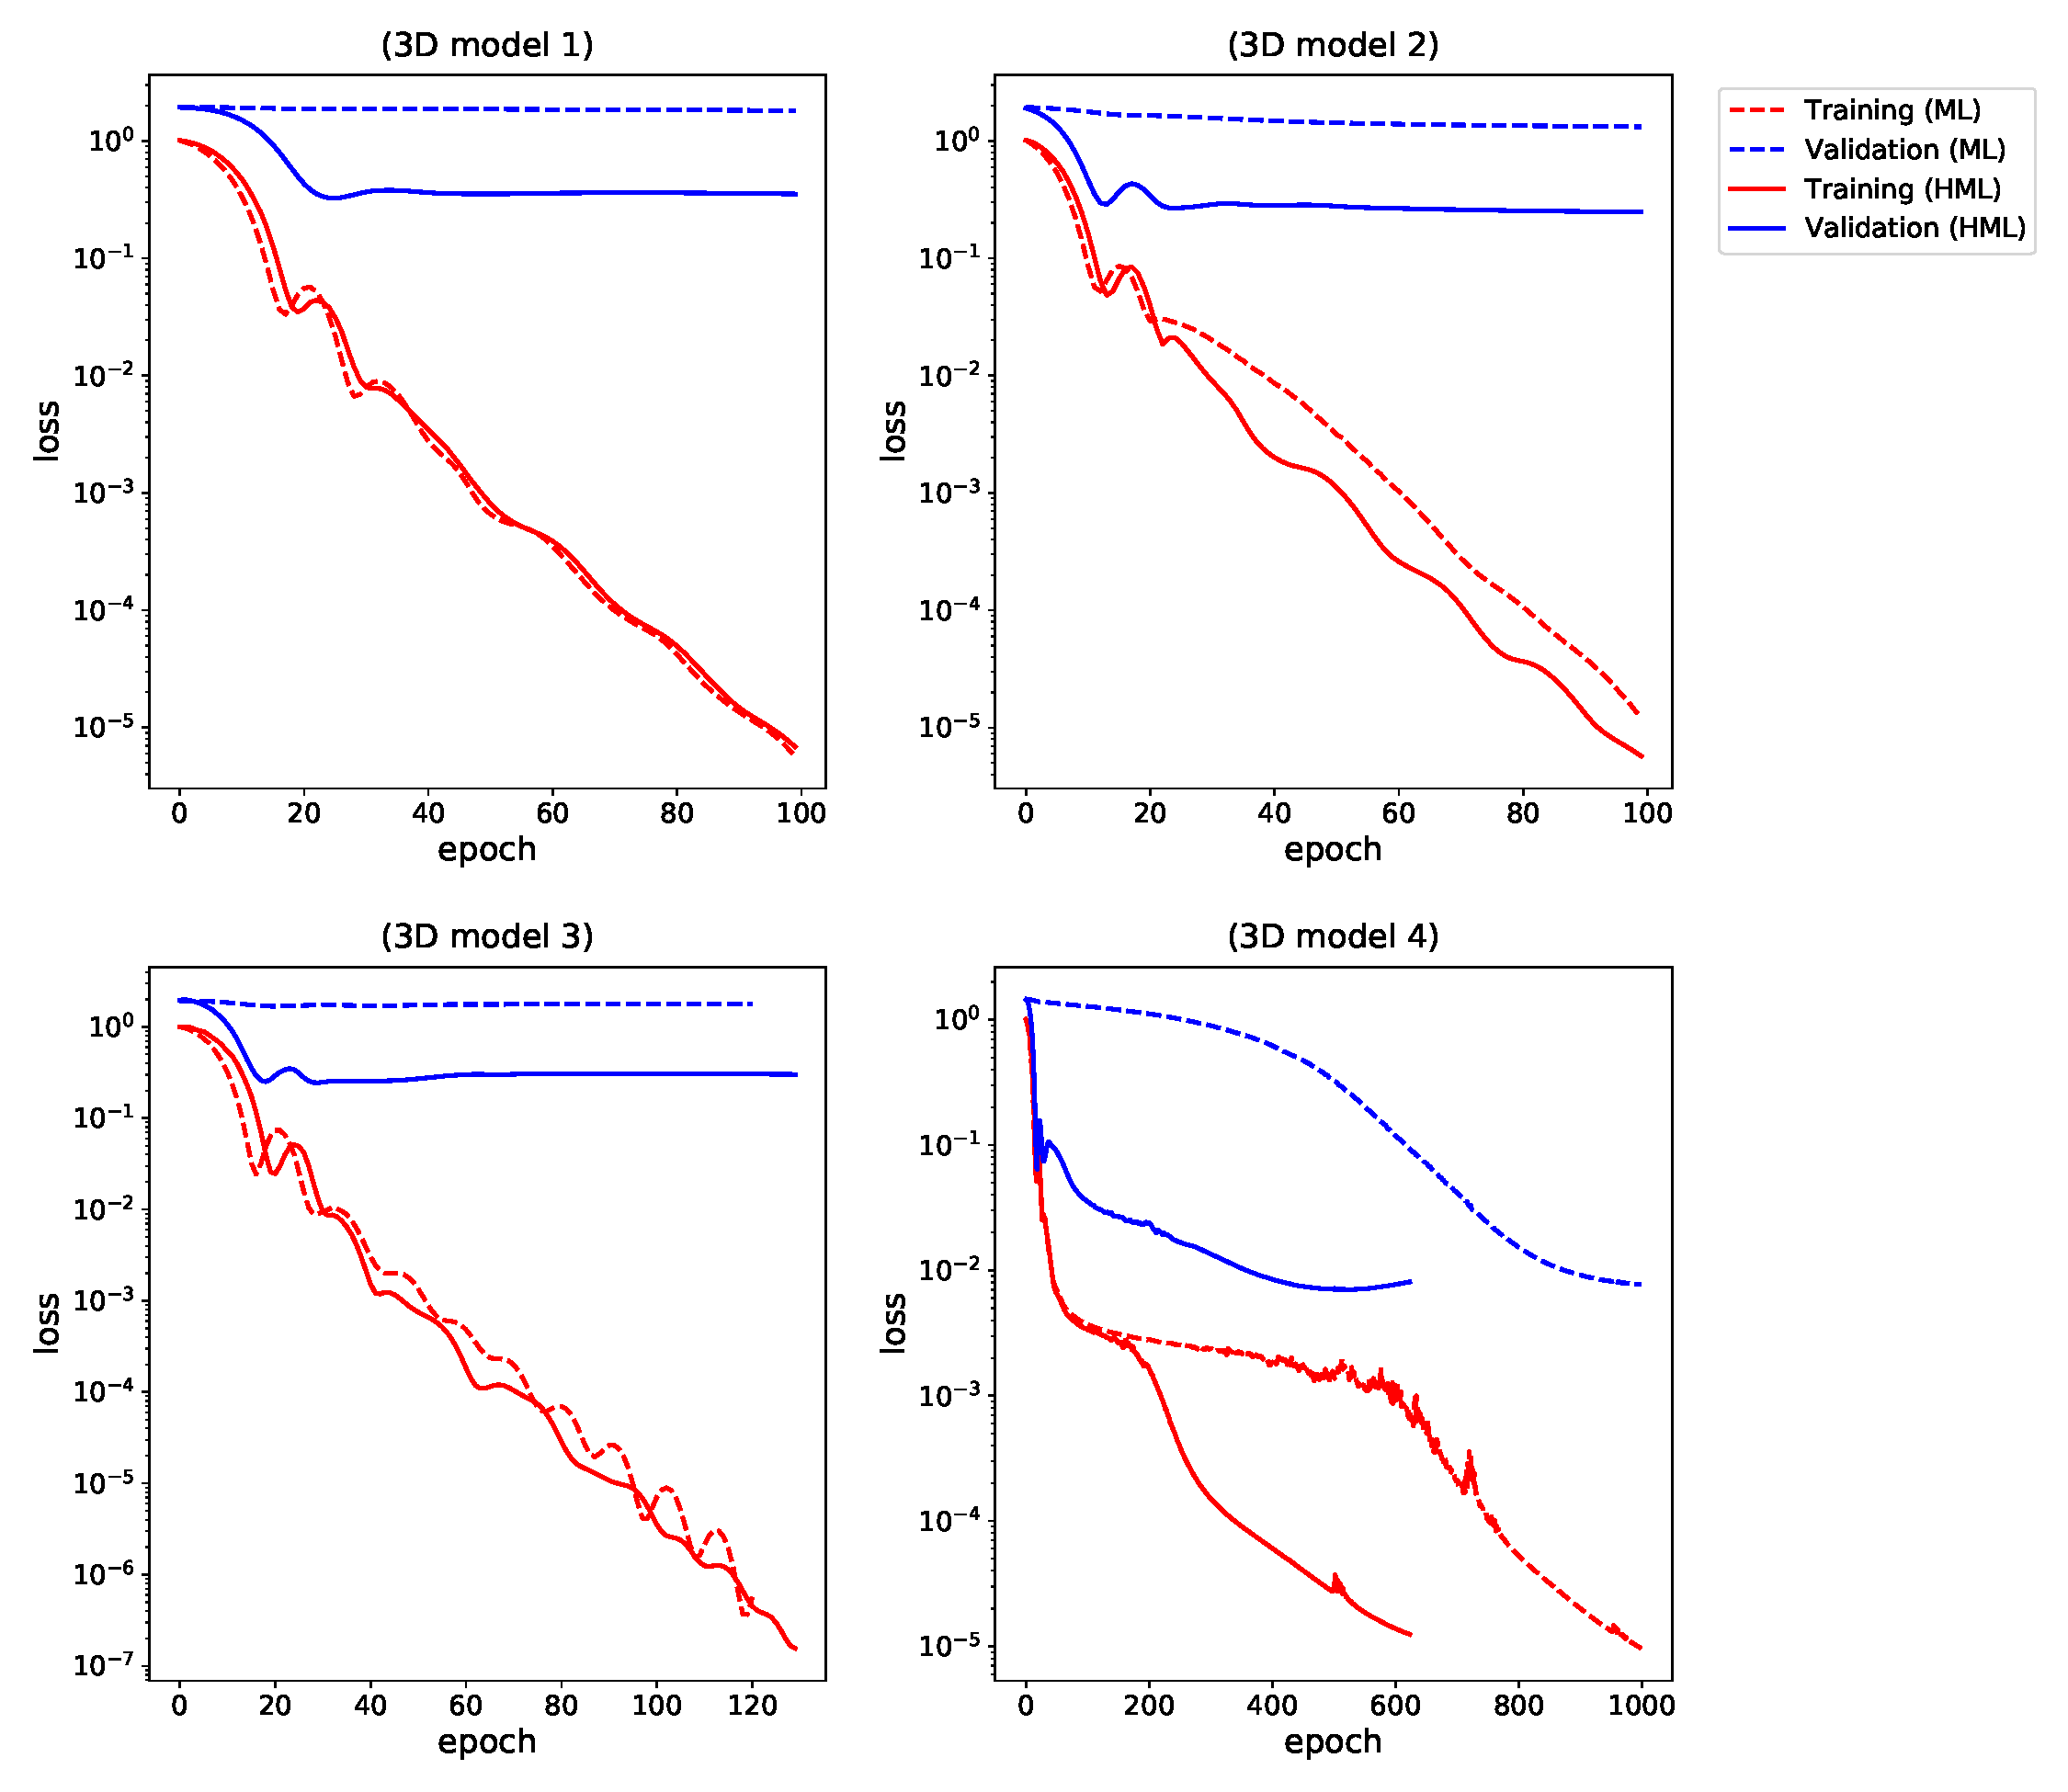
\includegraphics[trim={0.5cm 0.5cm 0.6cm 0cm},clip,width=\linewidth]{3d.pdf}
\caption{Comparative analysis of loss values against the number of epochs in 3D surrogate modeling. It is observed that certain models achieved convergence earlier owing to the existence of the early stopping mechanism.
\label{fig:3D}}
\end{figure}

Further exploration into the hybrid methodology was conducted through \ac{3d} model $3$ (as also summarized in Table~\ref{table:2d} for the loss values in the final epoch). This model replicated the training and validation sample sizes of its predecessors, but introduced significant modifications in the epochs and neurons count - a tenfold increase and decrease in the former and latter, respectively. Additionally, the ReLU function was utilized alongside an early stopping parameter set at $100$. Despite these alterations, the efficiency of training was maintained, even over an extensive number of epochs. However, it is noteworthy that these adjustments harmed the \ac{hml} performance, as evidenced by a surge in validation loss after approximately $30$ epochs, yet it still outperformed the \ac{ml} surrogate.
%
\begin{table}
\centering
\caption{Loss values at the final epoch on training and validation sets in 3D modeling.\label{table:3d}}
\begin{tabular}{lcccc}
\toprule
\textbf{Surrogate model} &  \textbf{3D model 1} &  \textbf{3D model 2} &  \textbf{3D model 3} &  \textbf{3D model 4} \\
\midrule
ML (Training)   &   0.0000057 &   0.0000123 &   0.0000006 &   0.0000096 \\
HML (Training)  &   0.0000068 &   0.0000057 &   0.0000002 &   0.0000125 \\
ML (Validation) &   1.8169936 &   1.3181295 &   1.7773948 &   0.0076983 \\
HML (Validation)&   0.3536258 &   0.2480008 &   0.3019600 &   0.0080819 \\
\bottomrule
\end{tabular}
\end{table}


For 3D model 4, the size of training and validation datasets was increased by a factor of three. We maintained hyperparameters akin to those in our first 3D model but extended the training to a maximum of $1,000$ epochs, and we used the early stopping criteria established in our third 3D model. This escalated the computational cost of our last 3D model significantly. Indeed, the increased data generation, more learnable parameters, and extended training duration led to a substantial increase in both training and computational time for numerical data generation. The findings indicate that both the \ac{ml} and \ac{hml} models yielded comparably consistent loss values upon convergence. Notably, the HML approach demonstrated a markedly faster convergence rate, recording a validation loss of $0.1$ within approximately $10$ epochs – approximately 75 times quicker than the ML model.

To further interpret the performance disparity observed between the models, Fig.~\ref{fig:visualization} presents a comparative analysis of the \ac{pmse} contours, applied to a reference state of one cartilage substructure. The first three ML models displayed suboptimal performance across various points, whereas their \ac{hml} counterparts achieved significantly higher accuracy levels, with minimal pointwise error outliers (evidenced by sparse small red areas). The fourth \ac{ml} model exhibited comparable accuracy levels to the \ac{hml} model, with minor differences. However, in this inefficient surrogate modeling scenario, there was also a greater frequency of pointwise errors, suggesting a preference for the other more efficient \ac{hml} models. Again, this analysis emphasizes the benefits of adopting \ac{hml} modeling techniques, particularly in scenarios with limited data availability.
%
\begin{figure}\centering
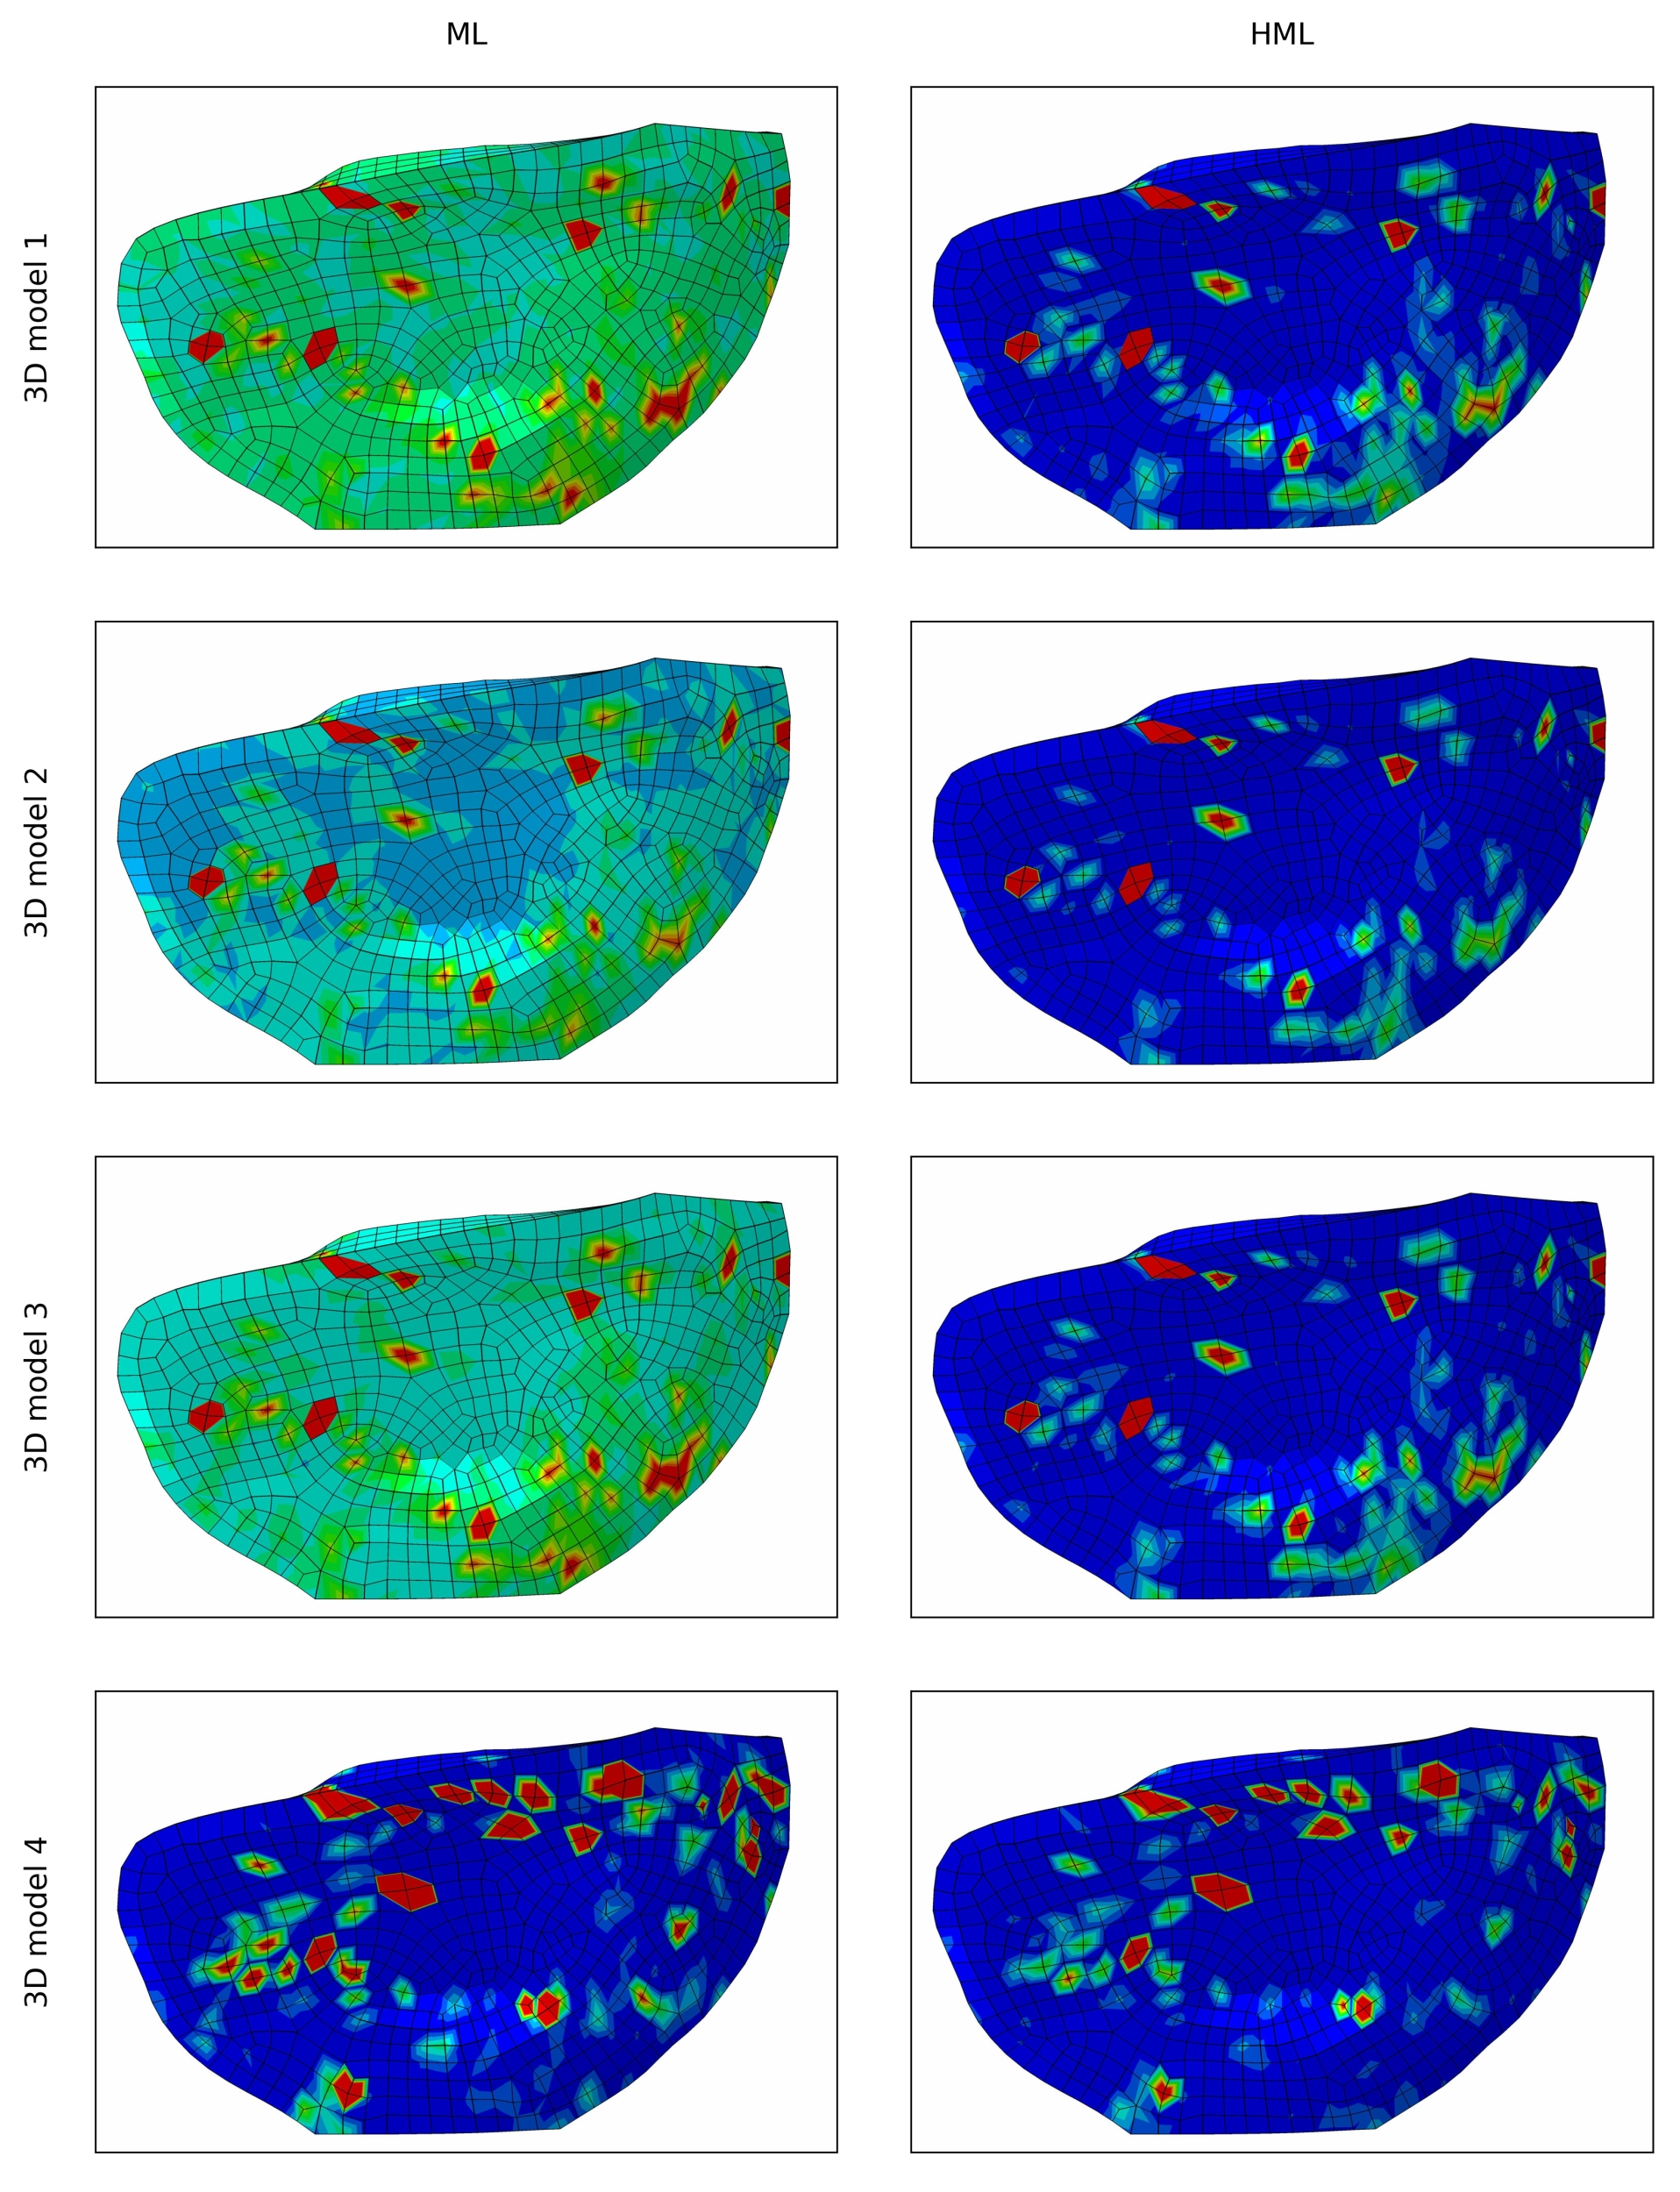
\includegraphics[height=0.9\textheight]{visualization_3d.jpg}
\caption{Illustration of PMSE contours for all three-dimensional surrogate models. Illustrated values are from zero (shown in blue) to beyond 2 (shown in red).}\label{fig:visualization}
\end{figure}

\paragraph{Other discussion.} This work acknowledges certain limitations. Firstly, we simplified the \ac{hf} numerical models for efficient data acquisition; however, this does not majorly impair the study as the simulations primarily aim to highlight the efficacy of the hybrid approach in biomechanical simulations in general, rather than serving as clinically validated \ac{ac} models. Secondly, the empirical experiments presupposed that the training phases should not substantially exceed the numerical data generation in cost, to justify the adoption of these surrogate models. Consequently, expensive settings for surrogate training were not employed. While this may restrict our findings to the specific conditions of our models, such presumptions are often necessary when utilizing surrogate models on regular hardware settings.

In summary, this chapter introduces an \ac{hml} methodology for multi-fidelity-based surrogate modeling and \ac{fe} analysis of cartilage-like soft tissues. The \ac{lf} model in this context is derived by simplifying the multi-physics formulations, making the \ac{mor} process relatively direct and non-invasive. Extensive empirical evaluations also reveal that our hybrid approach enhances training efficiency and improves the performance of surrogate modeling with minimal training data. This is particularly beneficial, as it overcomes the challenge faced by many existing \ac{ml}-based surrogate models that usually require numerous costly \ac{hf} samples.


\chapter{Efficient and Generalizable Learning for Surrogate Modeling}\label{ch5}
%
The effectiveness of our \ac{hml} in single-scale, few-shot learning has been demonstrated, with the \ac{gnn} model showing promise for generalizable learning. Our goal is to develop a multiscale surrogate model, trained on augmented tissue-scale data, capable of potentially achieving zero-shot generalizability for knee-scale simulations. This chapter introduces a novel, physically constrained perturbation method to \ac{da}, generating various elements, that might be seen in large-scale analyses using small-scale data. We also extend our hybrid algorithm with several preprocessing and customization algorithms, including the integration of an upstream \ac{ae} model to refine input features, and the application of feature transformation, resampling, and cost-sensitive functions to address data imbalances. This is complemented by a customized, memory-efficient framework that accelerates training. We test this approach using the advanced multiphasic model of cartilage, considering all its constituents, to evaluate the viability of this technique and compare it to its ablated versions (wherein certain extensions are disabled for the sake of comparison).

\section{Related Work}
%
\paragraph{Generalizable surrogate modeling.} The challenge of generalization in \ac{ml}-based surrogate models, especially for models involving different topologies, has been explored in few studies [\cite{hoffer2022,taghizadeh2020}]. A prominent approach to address this issue involves the integration of theory-inspired features or physics-constrained models. In particular, \cite{gao2021} successfully applied a theoretically-inspired feature engineering method to adapt their model from a regular to an irregular mesh. Also, \cite{nourbakhsh2018} developed a surrogate model for truss analysis utilizing domain-specific features to encapsulate various topologies. The complexity of integrating domain knowledge, especially in cartilage biomechanics, as pointed out in the previous chapter, favors the use of graph neural networks for their capability in generalizable modeling across different scales. This data-driven approach can employ the relational inductive biases [\cite{battaglia2018}], as successfully implemented in the single-scale 2D simulation of the previous chapter. Overall, such methods demonstrate potential, as facilitated multiscale generalization through their message-passing and local aggregation functions [\cite{battaglia2018,sanchez2020}].

Nonetheless, a primary challenge in training graph neural networks lies in their requirement for extensive message-passing steps, which can lead to prolonged training periods and the oversmoothing issue in downstream layers, where they become mostly identical and useless [\cite{zhang2024}]. A solution lies in limiting the message-passing iterations by adopting multi-level mesh resolutions, as extensively researched [\cite{cao2023,fortunato2022,li2020}]. Our hypothesis posits that the \ac{hml} technique could mitigate this challenge without relying on such complex input meshes. Additionally, we integrate an upstream \ac{ae} in our custom memory-efficient training loop, a widely adopted technique in surrogate modeling for tasks like reduced-order modeling or feature denoising [\cite{fresca2022,pant2021,fresca2021}], to possibly accelerate the training of our multiscale cartilage surrogate model.

\paragraph{Augmented graph data.} \ac{da}, the process of synthetically generating new data, is critical when dealing with limited datasets. Common augmentation methods include the application of generative models, noise addition, and the application of problem-related transformations such as rotations to the image data [\cite{mumuni2022}]. Such techniques have shown notable efficacy in enhancing model performance, particularly in physics applications where configuration-dependent tensors are utilized [\cite{cheung2023}]. Alternatively, the Mixup technique, involving the convex combination of sample pairs to interpolate new data, is another widely adopted method across various domains, including imaging [\cite{guo2019,zhang2018}], natural language processing [\cite{jindal2020,guo2020}], and graph data [\cite{han2022,wang2021}]. However, it has been mostly applied to graph classification rather than regression problems like surrogate modeling, an area where our technique offers a novel solution.

In the physics context, innovative, problem-specific augmentation techniques have been developed. More specifically, \cite{zhao2021} introduced a method in temperature prediction that exponentially increases training data by applying pairwise differences instead of absolute values. \cite{parida2023a} also augmented earthquake signals using a discrete wavelet transform method, creating new samples by perturbing the wavelet coefficients of original signals. Additionally, many surrogate models trained on image-based snapshots, e.g., [\cite{dong2022}]; thus employed random rotations to ensure orientation invariance, and in some multi-fidelity studies, e.g., [\cite{sella2023}], \ac{lf} training samples directly augment datasets. Our research particularly augments datasets for multiscale surrogate modeling without any large-scale data, a novel approach in this context.

\paragraph{Handling imbalanced data.} Given the skewed distribution prevalent in biomedical data [\cite{rauschenberger2020}], we hypothesized that our multiscale cartilage data necessitates specialized treatment to avoid uninformative representations biased towards common, simpler nodal representations. Traditional methods, such as applying logarithmic or cubic transformations based on the data distribution [\cite{bhattacharya2017}], help stabilize variance and reduce skewness. The Yeo–Johnson transformation [\cite{yeo2000}] represents a combined technique, defined by:
%
\begin{equation}\label{eq-yeo}
    \phi(x; \lambda) = \begin{cases} [(x + 1)^\lambda - 1] / \lambda & \text{if } \lambda \neq 0, x \geq 0, \\
\ln(x + 1) & \text{if } \lambda = 0, x \geq 0, \\
-[(-x + 1)^{2 - \lambda} - 1] / (2 - \lambda) & \text{if } \lambda \neq 2, x < 0, \\
-\ln(-x + 1) & \text{if } \lambda = 2, x < 0.
\end{cases}
\end{equation}
%
Here, $\phi$ is the transformed value of $x$ and $\lambda$ is a hyperparameter determined through maximum likelihood during data preparation. Other methods include maximal loss focusing on top error percentages and weighted loss, with the weights either statically assigned based on feature frequency [\cite{steininger2021}] or dynamically based on training errors [\cite{fernando2022}]. Resampling graph partitions or subgraphs depending on their importance, either statically by initial nodal feature distribution or dynamically by nodal error distribution during training, offers another solution. Although these methods are predominantly implemented in graph classification tasks [\cite{wang2022,zeng2020,chiang2019}], we have adapted them for our regression-based surrogate modeling problem.

\section{Methodology}
%
\subsection{Efficient and Generalizable Learning}
%
We initially try to balance and centralize the data to not only enhance training but also to ensure a fair evaluation. This is primarily achieved through the Yeo-Johnson transformation (eq.~\ref{eq-yeo}), along with other similar transformations that can be evaluated after delving into the data. Additionally, applying cost-sensitive and resampling strategies further complements this by compelling the trainer to focus more on the complex or rarer nodal points. The simplest solution is to utilize the maximal loss [\cite{shalev2016}], which restricts training to the top 10\% of the highest nodal errors.

Additionally, in our proposed methodology, each dimension of the dataset, denoted as \( \mathbf{D} \), is assigned a weight based on its frequency distribution. This process commences with the discretization of \( \mathbf{D} \) into \( n \) distinct bins. These bins are uniformly spaced according to the range of values present in \( \mathbf{D} \), defined by its minimum and maximum values. For a particular value \( d \in \mathbf{D} \), the corresponding bin index is represented by \( \text{bin}(d) \), and then the frequency \( f_i \) of the \( i^\text{th} \) bin is calculated as the inverse of the total count of elements in \( \mathbf{D} \) that are categorized within that bin. Subsequently, these frequencies are normalized to ensure their sum equals 1. This normalization process yields the final weight \( w_i \) for each value of the bin, which assuming we have $n$ bins, is calculated as:
%
\begin{equation}
    w_i = \frac{f_i}{\sum_{j=1}^{n} f_j}.
\end{equation}
%
In this context, \( \mathbf{D} \) can be seen as the original nodal input features, with a higher focus on the less frequent values that persist even after pre-preprocessing. Alternatively, \( \mathbf{D} \) could be dynamically assigned, based on the loss errors at each training epoch, to prioritize more complex nodes during the training phase. The weights thus assigned are then incorporated multiplicatively with the \( l_2 \) loss errors to implement a cost-sensitive function during training.

An alternative approach involves the application of subgraphing, i.e., sampling of the graph partitions, as illustrated in Fig.~\ref{fig:knee_inductive}. Studies, e.g., [\cite{you2020,sun2020,velickovic2018}], have shown that applying this may further increase consistency between local and global representation. We define a subgraph for each node before training, which is formed by identifying indices of neighboring nodes and edges. This identification is implemented through message-passing steps that accumulate the indices of the nodes and edges. Each subgraph of each node, called the central node, is then isolated based on the collected indices. Considering that graph partitioning can affect each neighboring node, the training errors are only computed on the central nodes, which aggregate all the unaffected information. The selection of these central nodes for subgraphing is guided by the calculated weights, now interpreted as sampling probabilities. The resampling can again be implemented statically and dynamically, as implemented for the cost-sensitive functions.
%
\begin{figure}\centering
\includegraphics[width=1\linewidth,keepaspectratio]{knee_inductive.png}
\caption{Example of a one-hop subgraph node, shown in red, interacting with neighboring nodes, shown in blue, within a numerical cartilage model. By subgraphing, the semantics can be preserved in the randomly selected central (target) nodes.}\label{fig:knee_inductive}
\end{figure}

On the other hand, we introduce a \ac{da} technique that perturbs each nodal feature, denoted as $\mathbf{T}$. This modification is inspired by the graph-based Mixup method [\cite{guo2023,park2022}] and nodal graph perturbation [\cite{gibson2022}] but is adapted to suit the nature of our spatiotemporal data, as follows:
%
\begin{equation}\label{eq-interpolation}
    \mathbf{T}_{\text{new}} = K \mathbf{T}_i + (1 - K)\mathbf{T}_j.
\end{equation}
%
Here, $K \in [0, 1]$ is a random value, $\mathbf{T}_{\text{new}}$ represents the newly created nodal feature. It is derived from a combination of features corresponding to two existing points, $\mathbf{T}_i$ and $\mathbf{T}_j$, located in the spatial axis and temporal space.

To implement our \ac{da}, we first need to identify and move a selected frame and node of the $i$-th point used for linear interpolation by randomly selecting $K$ at each point and selecting one of the closest points, i.e., the $j$-th point. Finding associated temporal frame points is straightforward: we simply select the closest pair of recorded temporal frames, in the temporal axis, and one of these points is then randomly replaced with the new point as long as it is not the initial or final frame points. Such methods are widely used in \ac{da} of time series [\cite{oh2020}], which now we implement on each node. However, the same approach does apply to \ac{da} of geometry. If we were to perturb nodal points randomly for later augmentation by interpolation, there is a risk that the new nodal points might fall outside the relevant geometry, generating invalid shapes, especially around contacting regions.

Our \ac{da} is capable of generating a valid shape, which may be present in large-scale simulations. This process is accomplished by randomly selecting one of the \textit{allowable} connecting edges at each node. Then, as illustrated in Fig.~\ref{fig:augmentation}, the selected edge is used to relocate the node, provided that it does not affect the boundary. Consequently, we define our associated $i$-th and $j$-th points (in this context, nodes) as the chosen node to be moved (essentially, to be replaced by a new node interpolated using the previously mentioned equation) and the node to which it is connected. This implies that the nodes are confined to moving along the selected allowable edges. Identifying these allowable edges is straightforward in a simple, small-scale model used for \ac{da}, as exemplified in the subsequent subsection.
%
\begin{figure}\centering
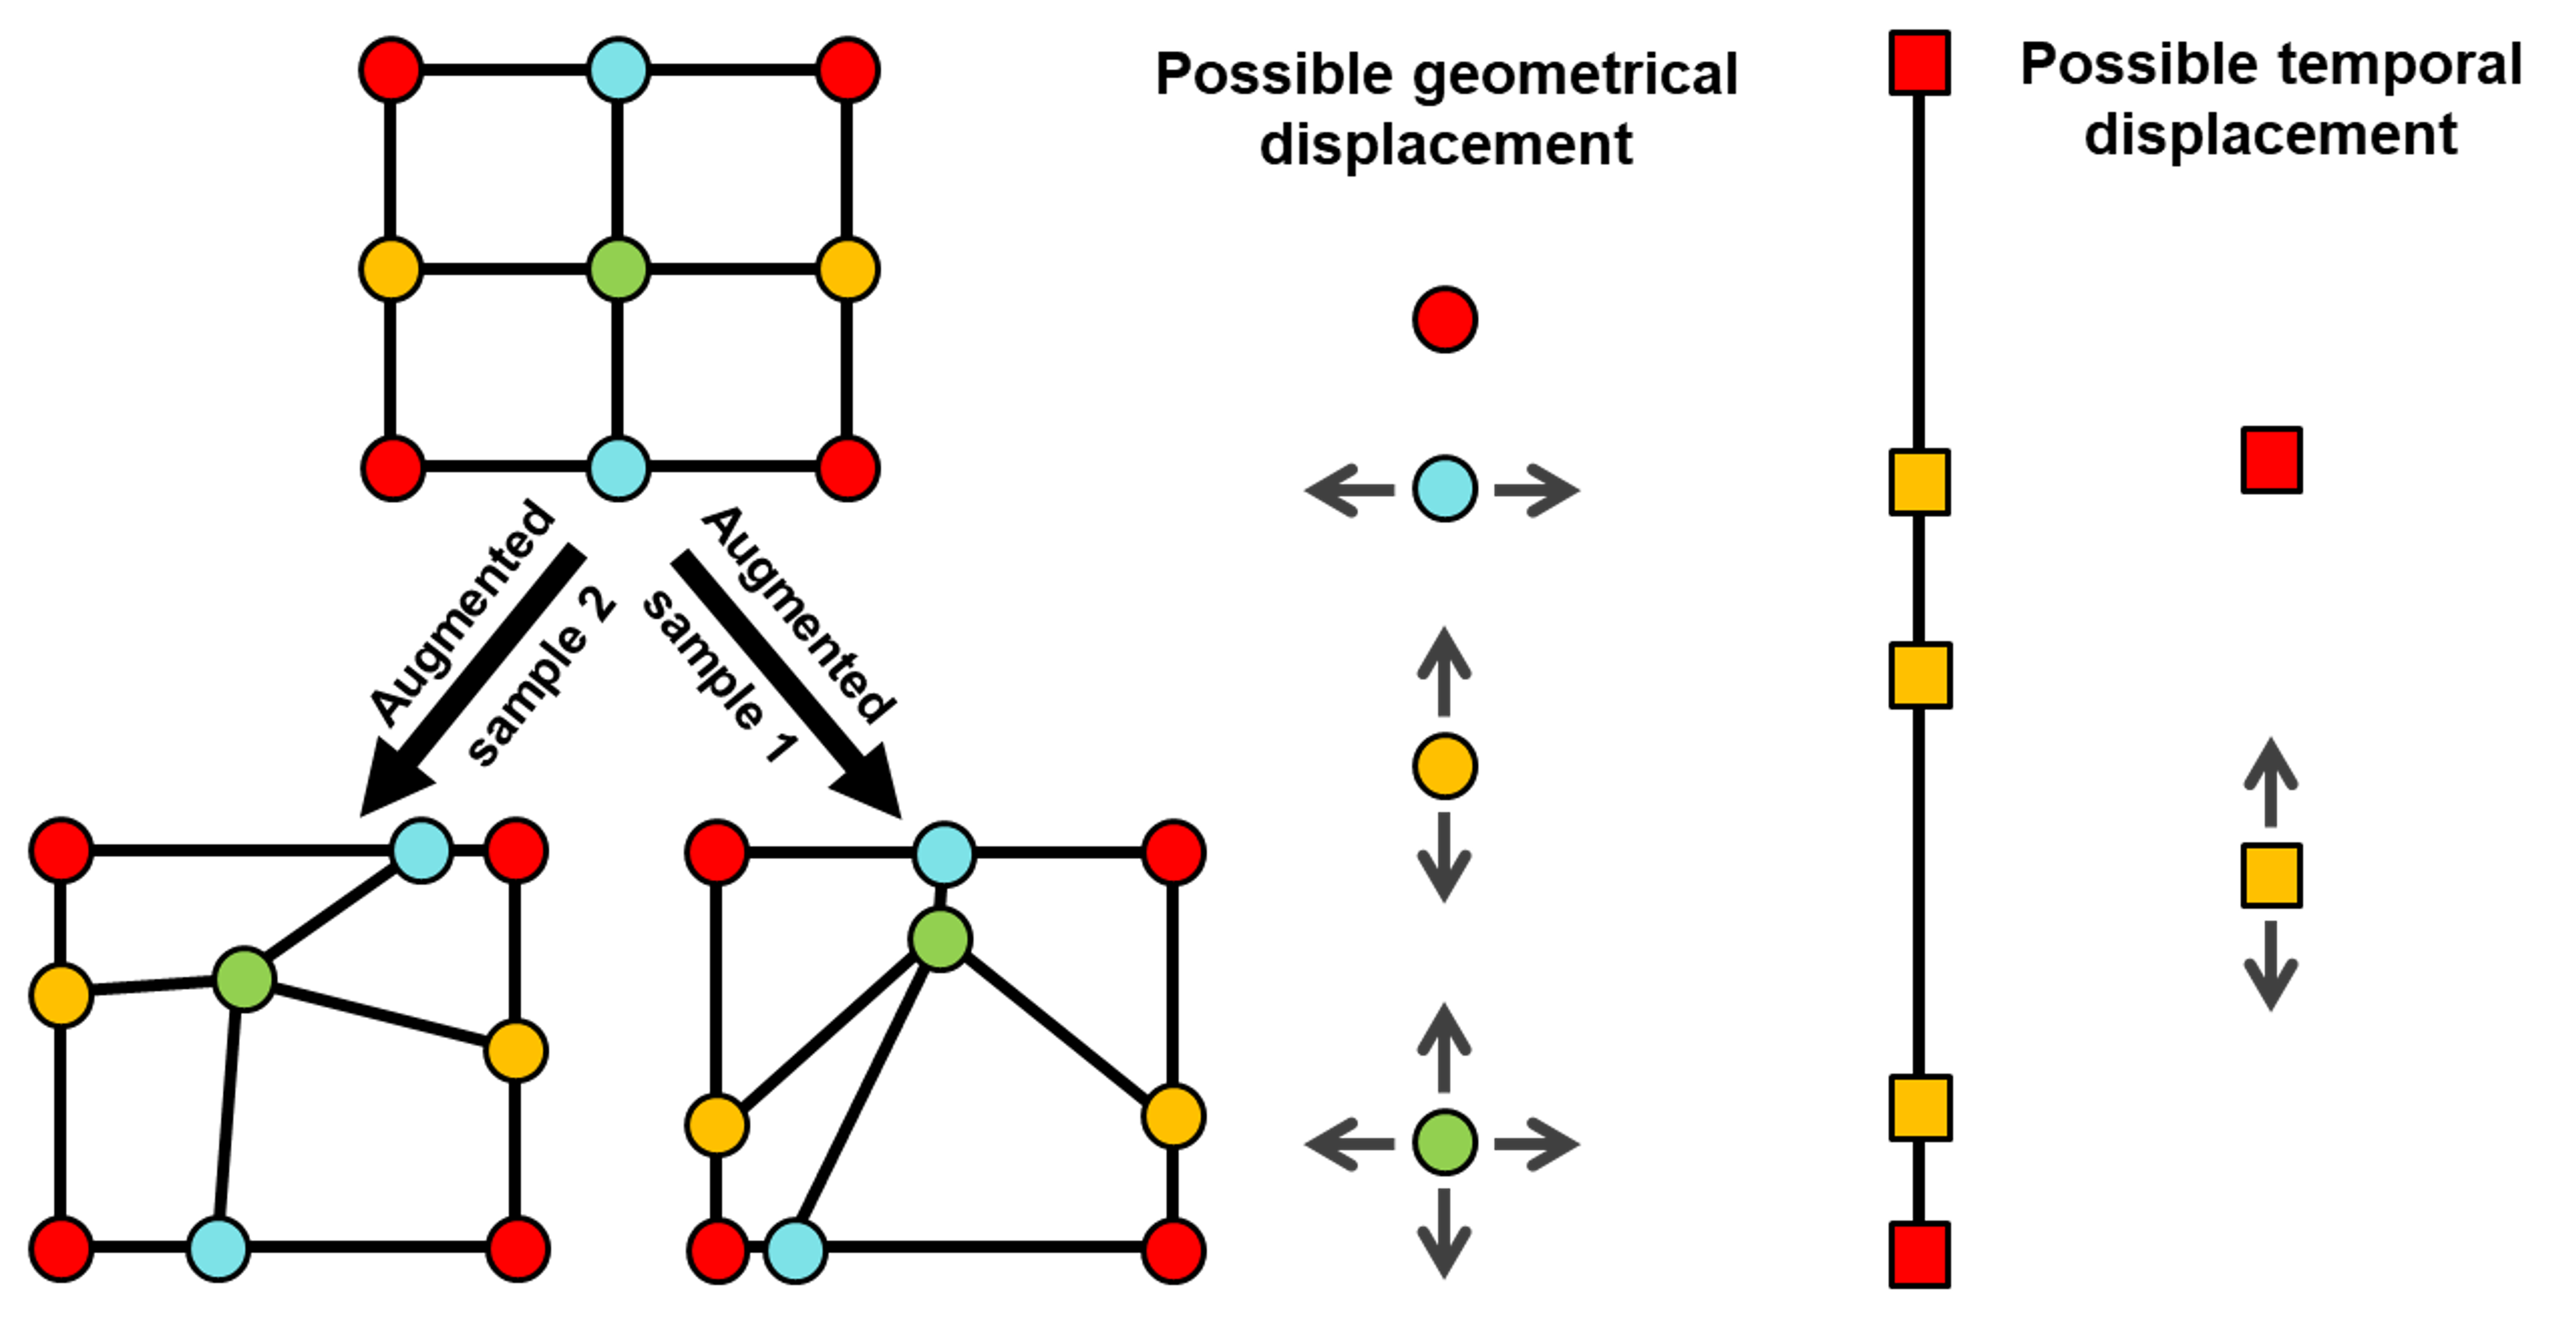
\includegraphics[width=0.8\linewidth,keepaspectratio]{augmentation.png}
\caption{Sample of data augmentation in the spatial and temporal domains, moved on possible or allowable directions.}\label{fig:augmentation}
\end{figure}

After the spatiotemporal perturbation, it is necessary to randomly rotate the coordinate axes using a randomly generated rotation matrix $\mathbf{R}$, as they might differ across scales. In this way, any component of data $\mathbf{T}$ can be rotated to $\mathbf{T}_\text{rotated}$, utilizing finite strain theory [\cite{gerhard-book}], as follows:

\begin{equation}
\mathbf{T}_\text{rotated} = \begin{cases}
\mathbf{R}^{T} \cdot \mathbf{T} \cdot \mathbf{R} & \text{if \textbf{T} is a symmetric 2nd-order tensor}, \\
\mathbf{T} \cdot \mathbf{R} & \text{if \textbf{T} is a 1st-order tensor or a vector}, \\
\mathbf{T} & \text{if \textbf{T} is a scalar or one-hot encoding}. \\
\end{cases}
\end{equation}
%
These sequential transformations can create new interpolated nodal data with perturbed element configuration during training, as exemplified in Fig.~\ref{fig:da_sample}. However, the use of such on-the-fly \ac{da} and as well as complex subgraphing may bottleneck training. One remedy is our hybrid implementation, as inserting a solver in the surrogate can significantly accelerate training. This is achieved by simplifying the learning problem, as illustrated in the previous chapter, and by facilitating the transfer of boundary information to central areas, potentially reducing the need for high message passing [\cite{um2020}].

We further accelerate training using a custom training loop, depicted in Fig.~\ref{fig:training_loop}.
%
\begin{figure}\centering
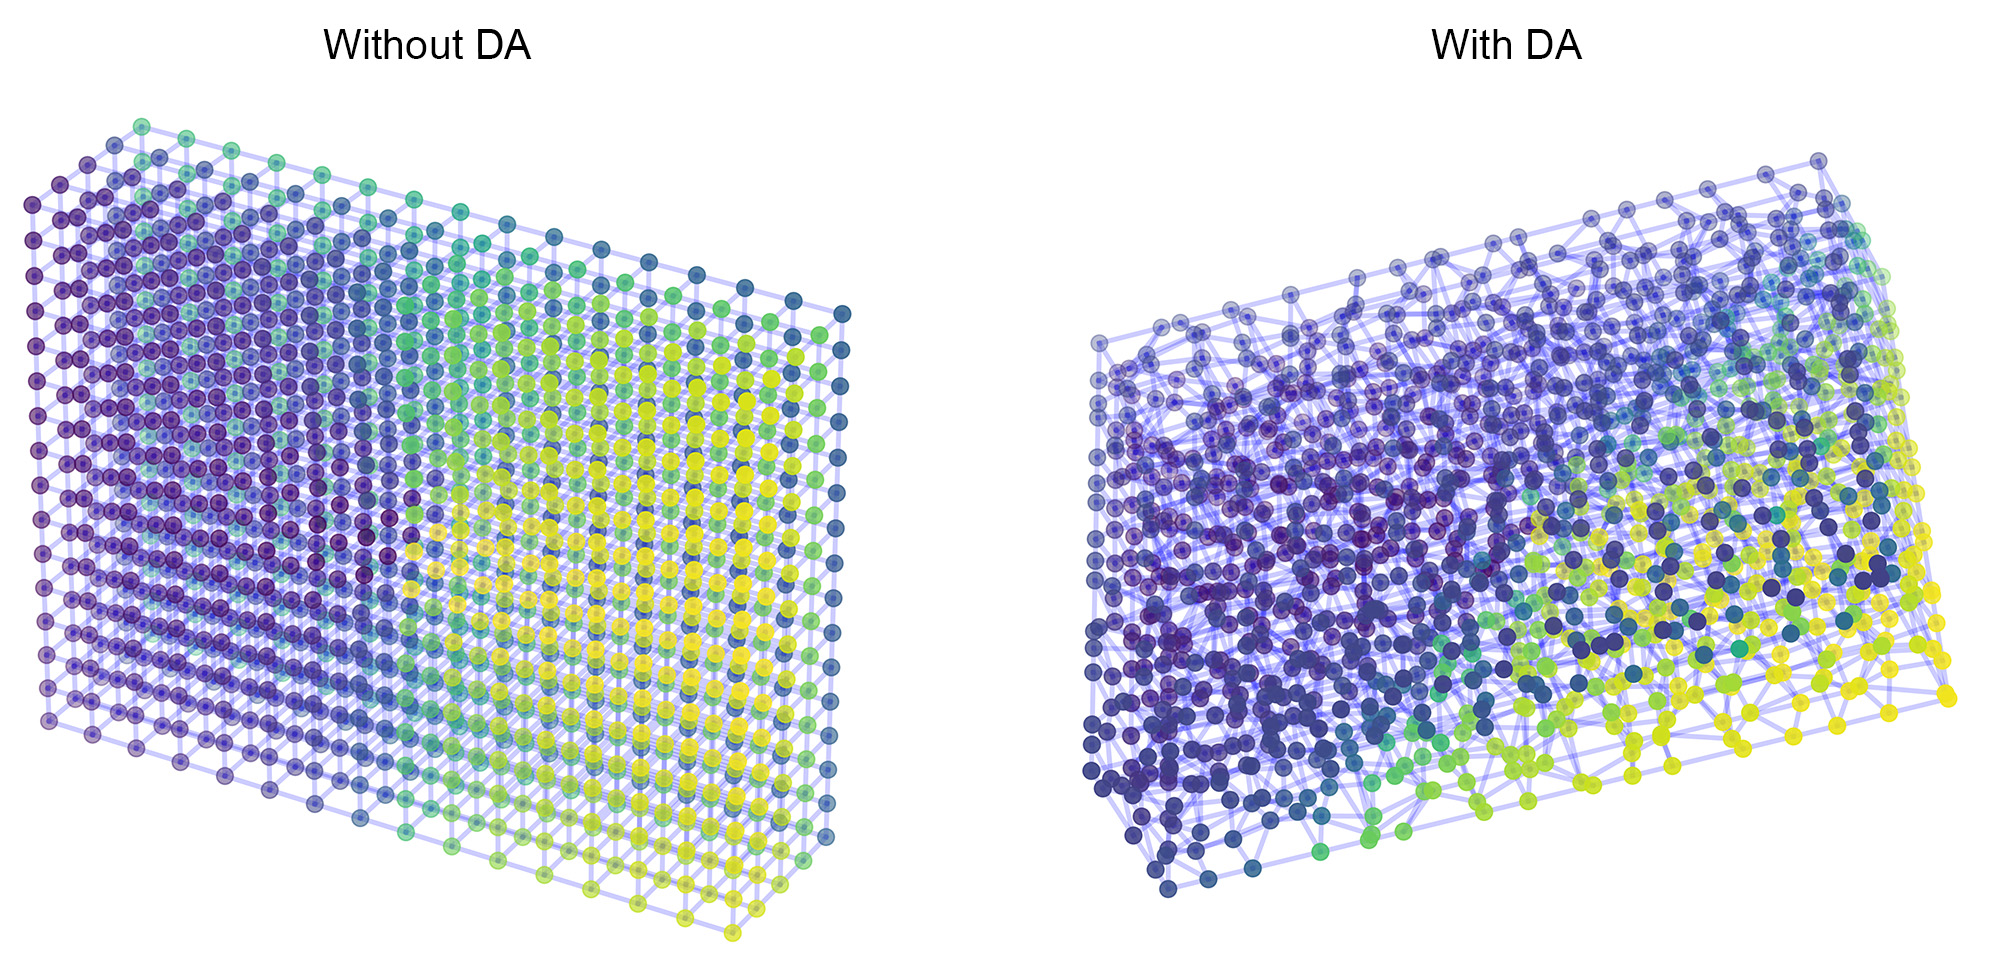
\includegraphics[width=0.8\linewidth,keepaspectratio]{da_sample.jpg}
\caption{Sample of a model with and without data augmentation.}\label{fig:da_sample}
\end{figure}
%
It implements each epoch of training with preprocessing and an early stopping algorithm, followed by another nested loop for training, also employing another early stopping. This process ensures new data is introduced only when necessary, thus speeding up training. Nonetheless, this incremental learning approach risks overshooting. To mitigate this, the algorithm decreases the learning rate, \( \alpha \), by a factor of 10 at the end of each epoch, and then progressively increases it in the nested loop, as follows:
%
\begin{equation}
    \alpha = \frac{1}{10^{i_{\text{outer}}}} \left[
    \alpha_{\text{init}} + \min\left(\frac{i_{\text{inner}}}{N_{\text{inner}}}, 1\right) \cdot (\alpha_{\text{final}} - \alpha_{\text{init}})
    \right].
\end{equation}
%
Here, \( i_{\text{inner}} \) and \( N_{\text{inner}} \) denote the iteration count and patience number of the secondary (inner) loop, respectively. \( i_{\text{outer}} \) represents the iteration count of the primary (outer) loop, i.e., the epoch number. \( \alpha_{\text{init}} \) and \( \alpha_{\text{final}} \) refer to the initial and final learning rate ranges in the first epoch. The optimal data is stored to be restored if overshooting occurs. Training terminates when the learning rate becomes significantly reduced. This methodology permits efficient implementation of our training experiments, even on a regular \ac{cpu}.
%
\begin{figure}\centering
\includegraphics[width=\linewidth,keepaspectratio]{training_loop.png}
\caption{Key stages of the custom training loop. The primary distinction from standard training loops is the incremental preprocessing of large batches of graphs at each epoch, coupled with iterative training within a separate inner loop for these large batches; thereby speeding up the training process. Additionally, the early stopping algorithms and learning rate schedulers are employed to prevent overshooting and overfitting, respectively.}\label{fig:training_loop}
\end{figure}

\subsection{Simulation Tests}
%
We systematically analyze the impact of \ac{da} and other proposed methods, focusing on the balance between generalizability and efficiency in complex biomechanical modeling. Initially, datasets are generated through small-scale simulations and subsequently tested in large-scale simulations, as depicted in Fig.~\ref{fig:inductive}.

%
\begin{figure}\centering
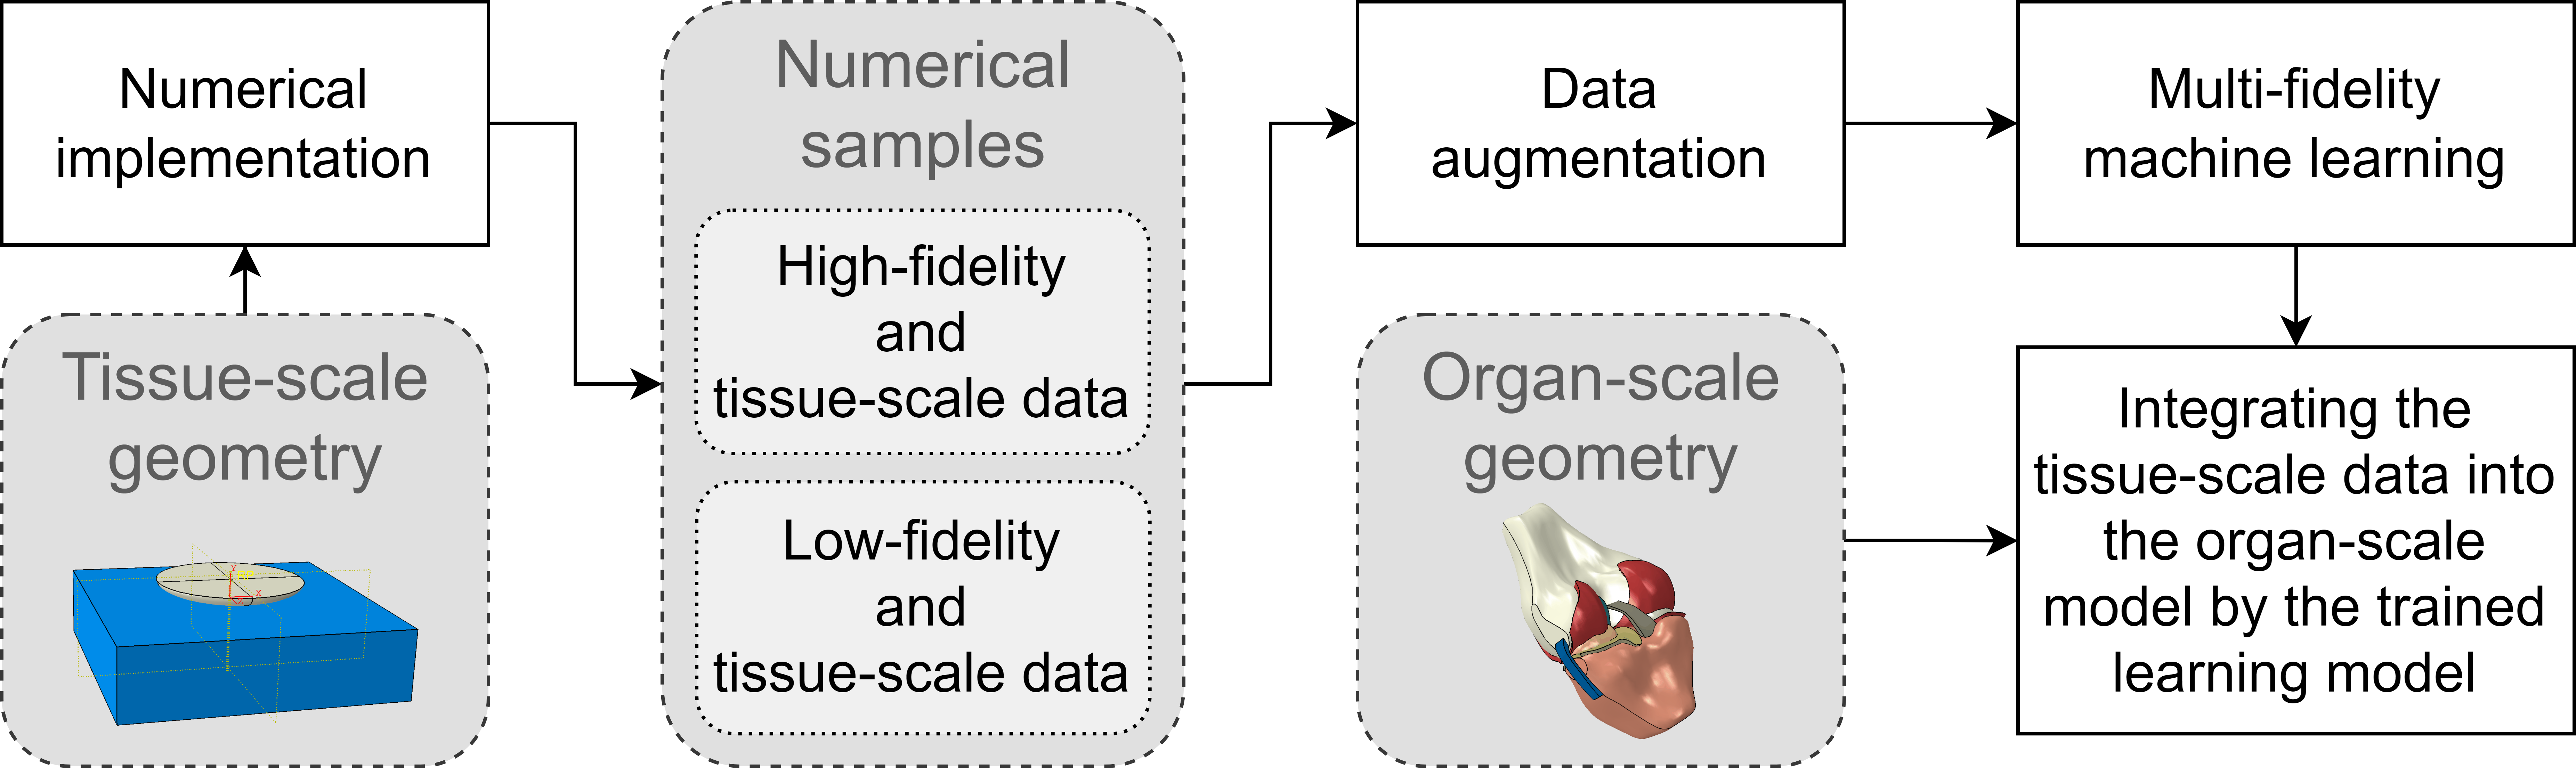
\includegraphics[width=1\linewidth,keepaspectratio]{inductive.png}
\caption{Illustration of the role of different models at different scales in surrogate modeling.}\label{fig:inductive}
\end{figure}

\paragraph{Dataset generation.} We implement the joint-scale model from the previous chapter, now enhanced with a complex multiphasic model for \ac{hf} modeling of cartilage. This includes all major components, as based on eqs.~\ref{eq-stress} and \ref{eq-cartilage_solid}. For the small-scale simulation, we employ a rectangular cube with dimensions $7.5\times7.5\times1.9\, \text{mm}^3$. This cube is subjected to compression by an indenter, mimicking the material behavior of soft tissue, here, a meniscus. In modeling cartilage at \ac{lf}, we assume linear viscoelasticity to capture the dynamic behavior of the tissue through a simpler monophasic model, based on eqs.~\ref{eq-isotropic_elastic} and \ref{eq-visco}. This is implemented using the 8-node linear brick elements, and we set $\mathcal{G}=0.744$, $\mathcal{K}=0.978$, and $\mathcal{T}=13.3\,\text{Sec}$. Additionally, Young's modulus and Poisson's ratio are set at $37.8\,\text{MPa}$ and $0.47$, respectively. These values, adapted from former cartilage research [\cite{keenan2013}], are modified to enhance numerical convergence and to increase elasticity, thereby enriching the global data in the nodes, facilitating the subsequent \ac{hml} analyses.

The indenter used in the model is semi-elliptic with radii of $2$ and $0.5 \, \text{mm}$. We apply random displacement boundary conditions at a central reference point, kinematically coupled to the flat surface of the indenter. The bottom of the model is fully fixed. By approximating the normalized depth from the top and bottom surfaces, it effectively mimics a simple cut of the tissue. This approach, which employs a few elements of highly structured shapes, accelerates data generation. Ideally, we should have allowed fluid diffusion on the free-contacting surfaces for better fidelity, but this is omitted to simplify the numerical implementation. For increased accuracy, the indenter could have been designed using cartilage material and various shapes to better simulate the effect of complex boundary conditions. While these assumptions may compromise biomechanical fidelity, we intend to design reproducible physics problems by complex multiphasic cartilage models with generalizable surrogate modeling, rather than creating a validated application-oriented biomechanical model of cartilage, which lies beyond the scope of this \ac{ml} study.

By applying randomly sampling from uniform distribution ($U$), we sample axial displacements of indented from $U(0, \, 0.6\,\text{mm})$, whereas planar displacements are sampled from $U(0.5, \, 0.5\,\text{mm})$, and rotational displacements are sampled from $U(-0.1, \, 0.1\,\text{rad})$. In our large-scale analysis, human weight is sampled by $U(0, \, -1000\,\text{N})$. For all scenarios, the simulation time is sampled between $U(0.001, \, 100\,\text{Sec})$ to simulate different strain rates. Additionally, the rate of boundary conditions in small-scale simulations is further randomized with four weighting multipliers that are equally spaced in time, sampled from $U(0, \, 1)$. These weights are interpolated over the entire time range using a cubic spline interpolator [\cite{de_boor1978}], to minimize extreme variations. During implementation, we begin with the \ac{hf} models, recording also the time points for temporal synchronization between models of different fidelities. The \ac{hf} model outputs include fluid pressure and the Mises stresses of solid components, which serve as nodal target values. The stress-strain results, derived by the \ac{lf} model, along with the primary fibrillar directions, are used as input nodal features and are stored for use as nodal features. We also store time and one-hot encoded data, distinguishing surface nodes from others, as additional input nodal features.

We also identify the allowable edges for each node for \ac{da} in the small-scale model. These could be manually preselected and stored due to the simplicity of its geometry. However, we develop a simple algorithm that aggregates the indices of each connected edge and then ranks them by their quantity. Nodes with fewer edges (e.g., corner nodes) are considered fully fixed during \ac{da} (i.e., all their edges are non-allowable). Conversely, nodes with the most edges (e.g., inner nodes) have all their edges set as allowable for \ac{da} to enable nodal movements on them. For other nodes, edges connected to higher-ranked nodes are assumed non-allowable to maintain boundary shape unchanged. We store this nodal set of allowable edges for random selection during \ac{da} preprocessing.

We generate 50 small-scale samples, divided into three roughly equal groups: training, validation, and in-distribution testing samples. Out-of-distribution samples are generated from six far more resource-intensive large-scale simulations. To expedite the simulation process, we applied an arbitrarily large value for the maximum allowable change in fluid pressure, a method occasionally employed in similar cartilage studies (see, e.g., the \cite{mononen2023} study).

\paragraph{Training experimentation.} We first extracted the preprocessing hyperparameters used for normalization and Yeo-Johnson transformations, based on samples from the graphs generated for each numerical sample in the training set. The edge features, also normalized, are formulated as described in the previous chapter. In our on-the-fly preprocessor, we create graphs across all temporal frames for subsequent frame sampling. Our experiments include sampling one and two randomly selected closely located or interpolated frames (for 2 and 5 message passings respectively), which are concatenated to augment nodal and edge features. Then, \ac{da} is applied to these graph frames, with their relative temporal distances added as additional nodal input feature values. All these graphs are combined using disjoint unions of 100 sampled frames to create a large discrete graph batch for training.

We also experiment with application of different loss functions and subgraph resamplings, as will be reported in the following section. Additionally, a small Gaussian noise with a standard deviation of 0.01 was added to the nodal features. For further exploration, we experimented with models where an upstream \ac{ae} with a single compressive layer was used to encode input features. A \ac{cr} is utilized to report the ratio of the original input nodal features to the output size of the first latent layer. The primary and secondary patience hyperparameters are set to $2$ and $100$ respectively. Training commences with an initial learning rate of $0.1$, and is stopped when it reduces to less than $10^{-5}$. Finally, for resampling, we employed $1000$ subgraphs summed in each batch. To obtain sample or resampling weights, we used 50 bins for dynamic implementation, while 2 bins were employed for static implementation to avoid the curse of dimensionality. Other hyperparameters remained consistent with those used in the previous chapter.

For the evaluation, we also consider scenarios excluding our proposed methods, all evaluated by \acp{mse} and \acp{pmse}, applied to transformed targets. This approach ensures a fair comparison when averaging all outputs. It should be noted that the targets might be imbalanced and have highly varied ranges, which can significantly impact both learning and evaluation, as demonstrated in previous studies. However, with the preprocessing transformation, the targets' ranges are transformed into similar normalized distributions, and given that we also employ a cubic transformation, the error is highly influenced by even small potential nodal errors. Consequently, we set the training settings to achieve an error between than $0.1$ and $0.001$, as greater accuracy might be excessively costly and unnecessary, considering the inherent errors in numerical models which are, by nature, approximate.

Furthermore, while the in-distribution testing batch size remains 100, the out-of-distribution batch size is reduced to 5 since it hardly fits into memory due to the large scale of the knee model and complex preprocessing. This might influence the evaluation results from sampling; however, in most cases when interpreting the results, we focus on the overall pattern and disregard outliers, instead of considering a single sample that can be too simple or complex and not representative of the overall accuracy and generalizability. 

Obviously, the hyperparameters, training settings, and even \ac{fe} modeling might be further modified to enhance performance. In particular, in our experiments, we set them in a way to ensure overall fair comparisons, as in large batch sizes they all trained efficiently. Although we do not disregard the possibility that they might outperform with smaller batches, this makes experimentation infeasible under such different conditions. Yet, as will be shown, we still achieved sufficiently good accuracy with our extension.

While we have explained the implementation steps, interested readers can refer to the open-sourced repository\footnote{\href{https://github.com/shayansss/ehml}{https://github.com/shayansss/ehml}.} for further details.

\section{Results and Discussion}
%
In order to evaluate the generalizability of the extended \ac{hml} approach in cartilage biomechanics, a series of simulation tests were performed. These tests utilized varying fidelities and scales and were executed on a regular computing setup (a Core i5 \ac{cpu}). Detailed runtime metrics are presented in Tables~\ref{table:smallscale_runtime} and \ref{table:largescale_runtime} in Appendix \ref{appendix_1}, with a summary provided in Table~\ref{tabel:runtimes_stats}.
%
\begin{table}[H]
\caption{Runtimes (Min) with their mean and standard deviation for each model.}\centering
\label{tabel:runtimes_stats}
\begin{tabular}{lcc}
\toprule
 & \textbf{Small-scale simulation} & \textbf{Large-scale simulation} \\
\midrule
HF model & 21.21 ± 2.16 & 118.31 ± 6.42 \\
LF model & 1.31 ± 0.69 & 3.07 ± 0.27 \\
\bottomrule
\end{tabular}
\end{table}

A notable observation is the significant reduction in runtime compared to the efficiency gains recorded in the previous chapter, as, here, all the main components of cartilage are included in the simulation. This results in relative differences in runtime ranging from 15 to 38 times across different fidelities. Furthermore, the large-scale simulations exhibited slower performance, approximately 2 to 5 times, rendering the small-scale models more favorable choices for training. This discrepancy in runtime could potentially be amplified with the implementation of more complex boundary conditions in the knee models. Overall, the \ac{lf} models are efficient in all scales, justifying the applicability of the generalizable and hybrid machine learning framework of this study.

In this section, we report a series of comparative analyses to evaluate the effectiveness of extended \ac{hml} with and without the proposed extensions. The evaluations are performed across different simulation scales, while we use small-scale samples for training purposes. The \ac{ml} models are trained on a \ac{gpu}, while in parallel, preprocessed on a \ac{cpu} in a few hours. Nonetheless, they could have been implemented sequentially on a regular \ac{cpu}.

\paragraph{Tissue-scale simulation.} Prior to the training phase, a comprehensive preprocessing analysis is conducted on the nodal data of both inputs and outputs. This analysis is executed using various transformations, both individually on the ablated pipeline and in combination. The observed imbalance and skewness support our first hypothesis about the existence of such data, as shown in Fig.~\ref{fig:normalization}. We addressed this using a series of transformations, as such data might have led to biased training and reduced performance [\cite{rezvani2023}].
%
\begin{sidewaysfigure}
    \centering
    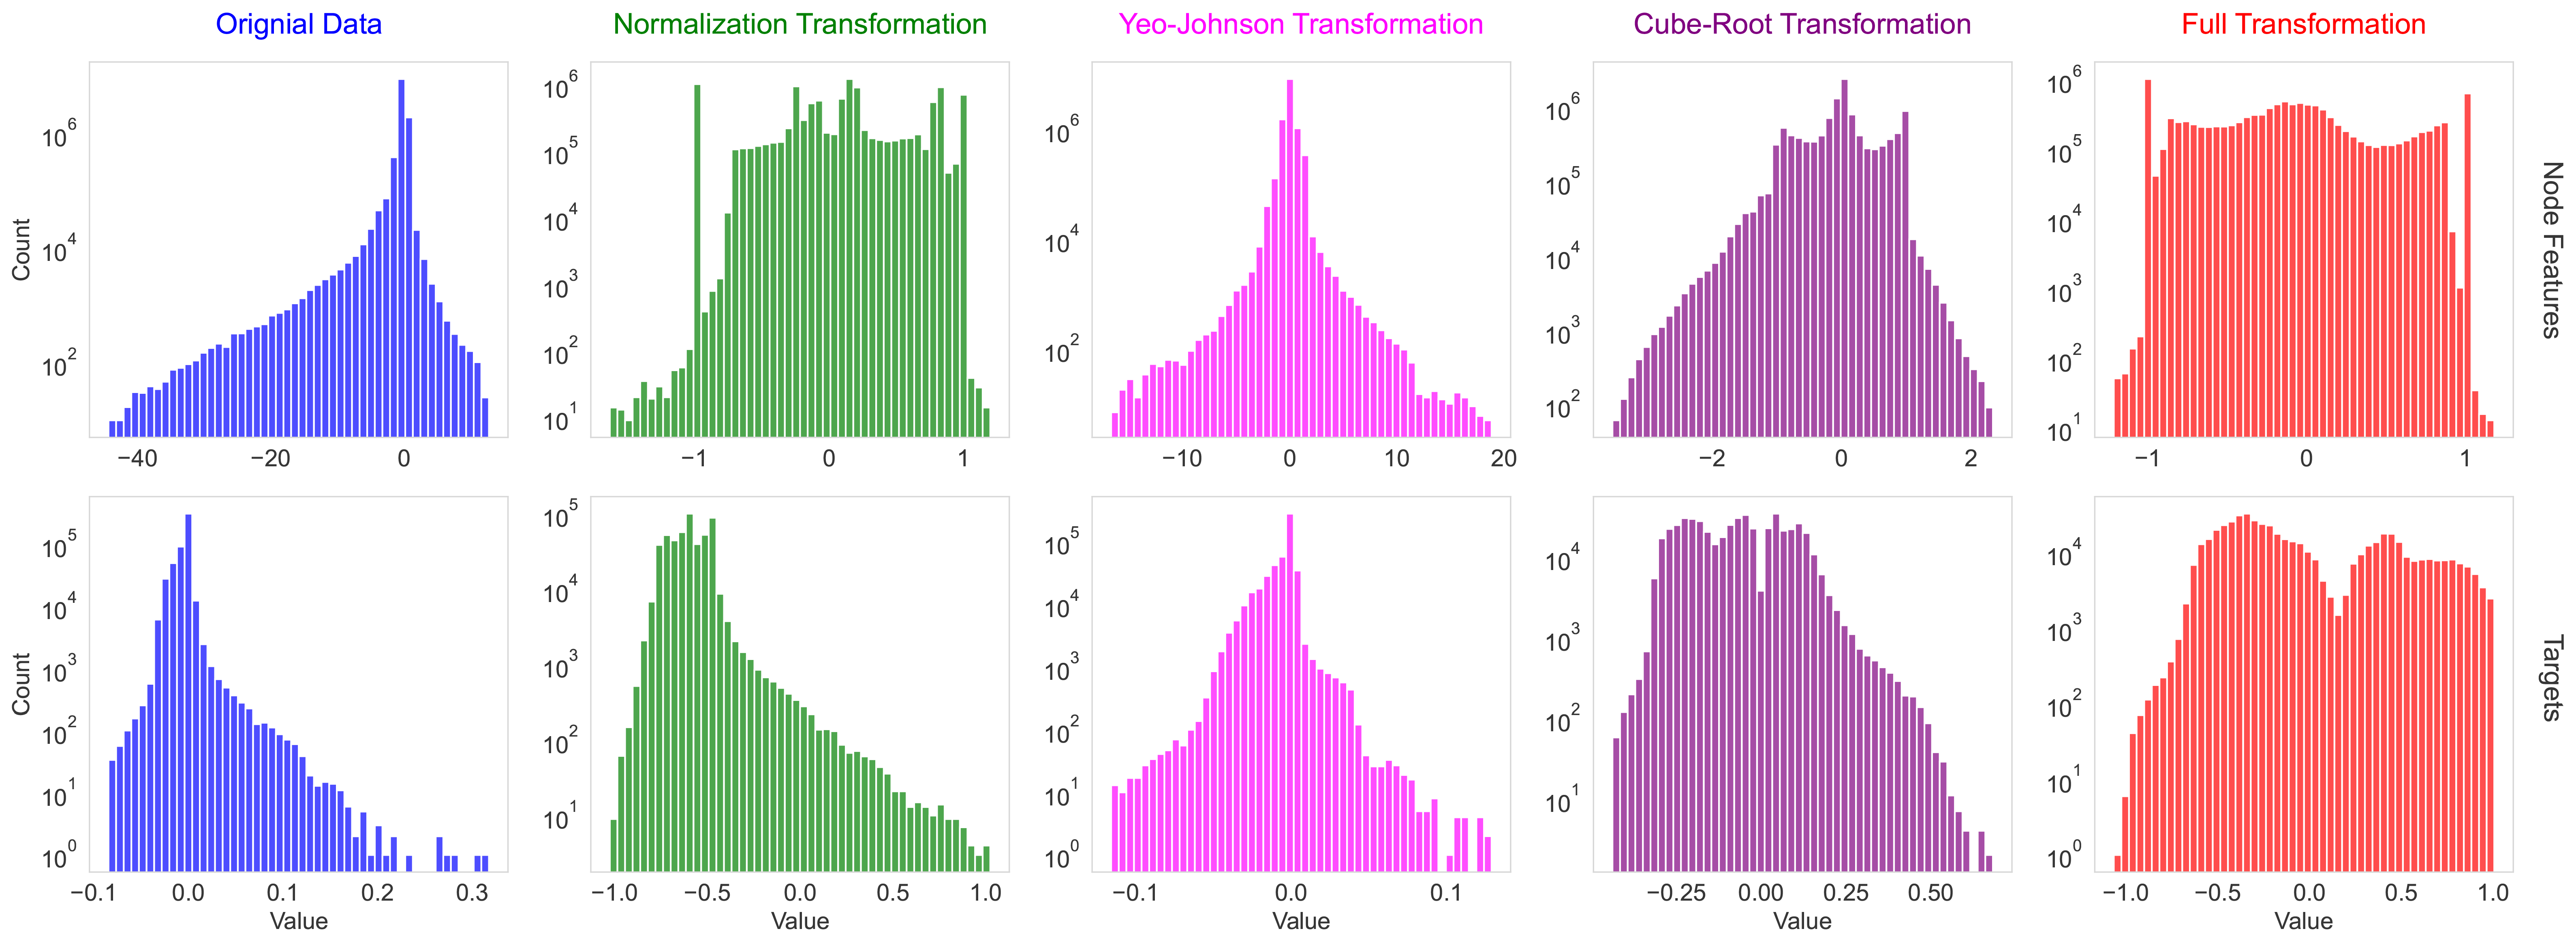
\includegraphics[width=\textheight,keepaspectratio]{normalization.png}
    \caption{Comparison of various preprocessing transformations on nodal input and output features. These transformations were applied to each feature dimension independently but were aggregated here solely for illustration purposes. Overall, the transformations alone could provide a more standardized normalized distribution, while their combination yielded a more uniform distribution. This approach can make the average evaluation errors highly sensitive to a small minority of complex nodes, rather than the majority of simpler nodes, which are typically in areas far from the boundaries (having small values). The existence of many small but few large values is attributable to the nature of soft tissues, where only small regions deform and resist pressure significantly more than other areas, particularly when the deformation is moderate but applied rapidly, as implemented in this study.}
    \label{fig:normalization}
\end{sidewaysfigure}

As expected, the normalization transformation diminished well data imbalance, yet it fell short in rectifying the skewness inherent in the data. Conversely, the Yeo-Johnson transformation demonstrates a marked improvement in centering the data, especially for the input features. Its combination with the normalization transformation could then potentially normalize the dataset and mitigate skewness. However, a notable imbalance persists, predominantly around the zero value, likely representing unaffected cartilage regions. The introduction of a cubic transformation, in conjunction with the aforementioned methods, shows potential in further refining the dataset. This approach not only addresses the remaining imbalances but also contributes to a more uniform data distribution, thereby preparing it for effective training and fair evaluation.

Figures~\ref{fig:gnn} and \ref{fig:combined} elucidate the training validation \acp{mse}, with and without \ac{ae}. Likewise, the testing \acp{mse} are averaged and detailed in Tables~\ref{table_in_distribution_2} and \ref{table_in_distribution_5} in Appendix~\ref{appendix_b}. It is observed that, in a majority of instances, a single graph batch (implemented repeatedly in one training epoch) is sufficient to attenuate the errors to negligible magnitudes. Exceptions are the models with lower \ac{cr} and more complexity, where feeding more training batches are still beneficial. Intriguingly, the integration of an upstream \ac{ae} did not yield an enhancement in training. In contrast, conventional loss functions exhibited superior performance, predominantly in complex models with more message-passing steps. Nevertheless, it is imperative to note that such enhancements do not imply improved generalization capabilities (as will be discussed). On a broader spectrum, the testing (in-distribution) errors predominantly align within comparable ranges, thereby supporting our hypothesis that the application of \ac{hml} allows opting for simpler models, allowing faster training [\cite{tan2021}].
%
\begin{figure}\centering
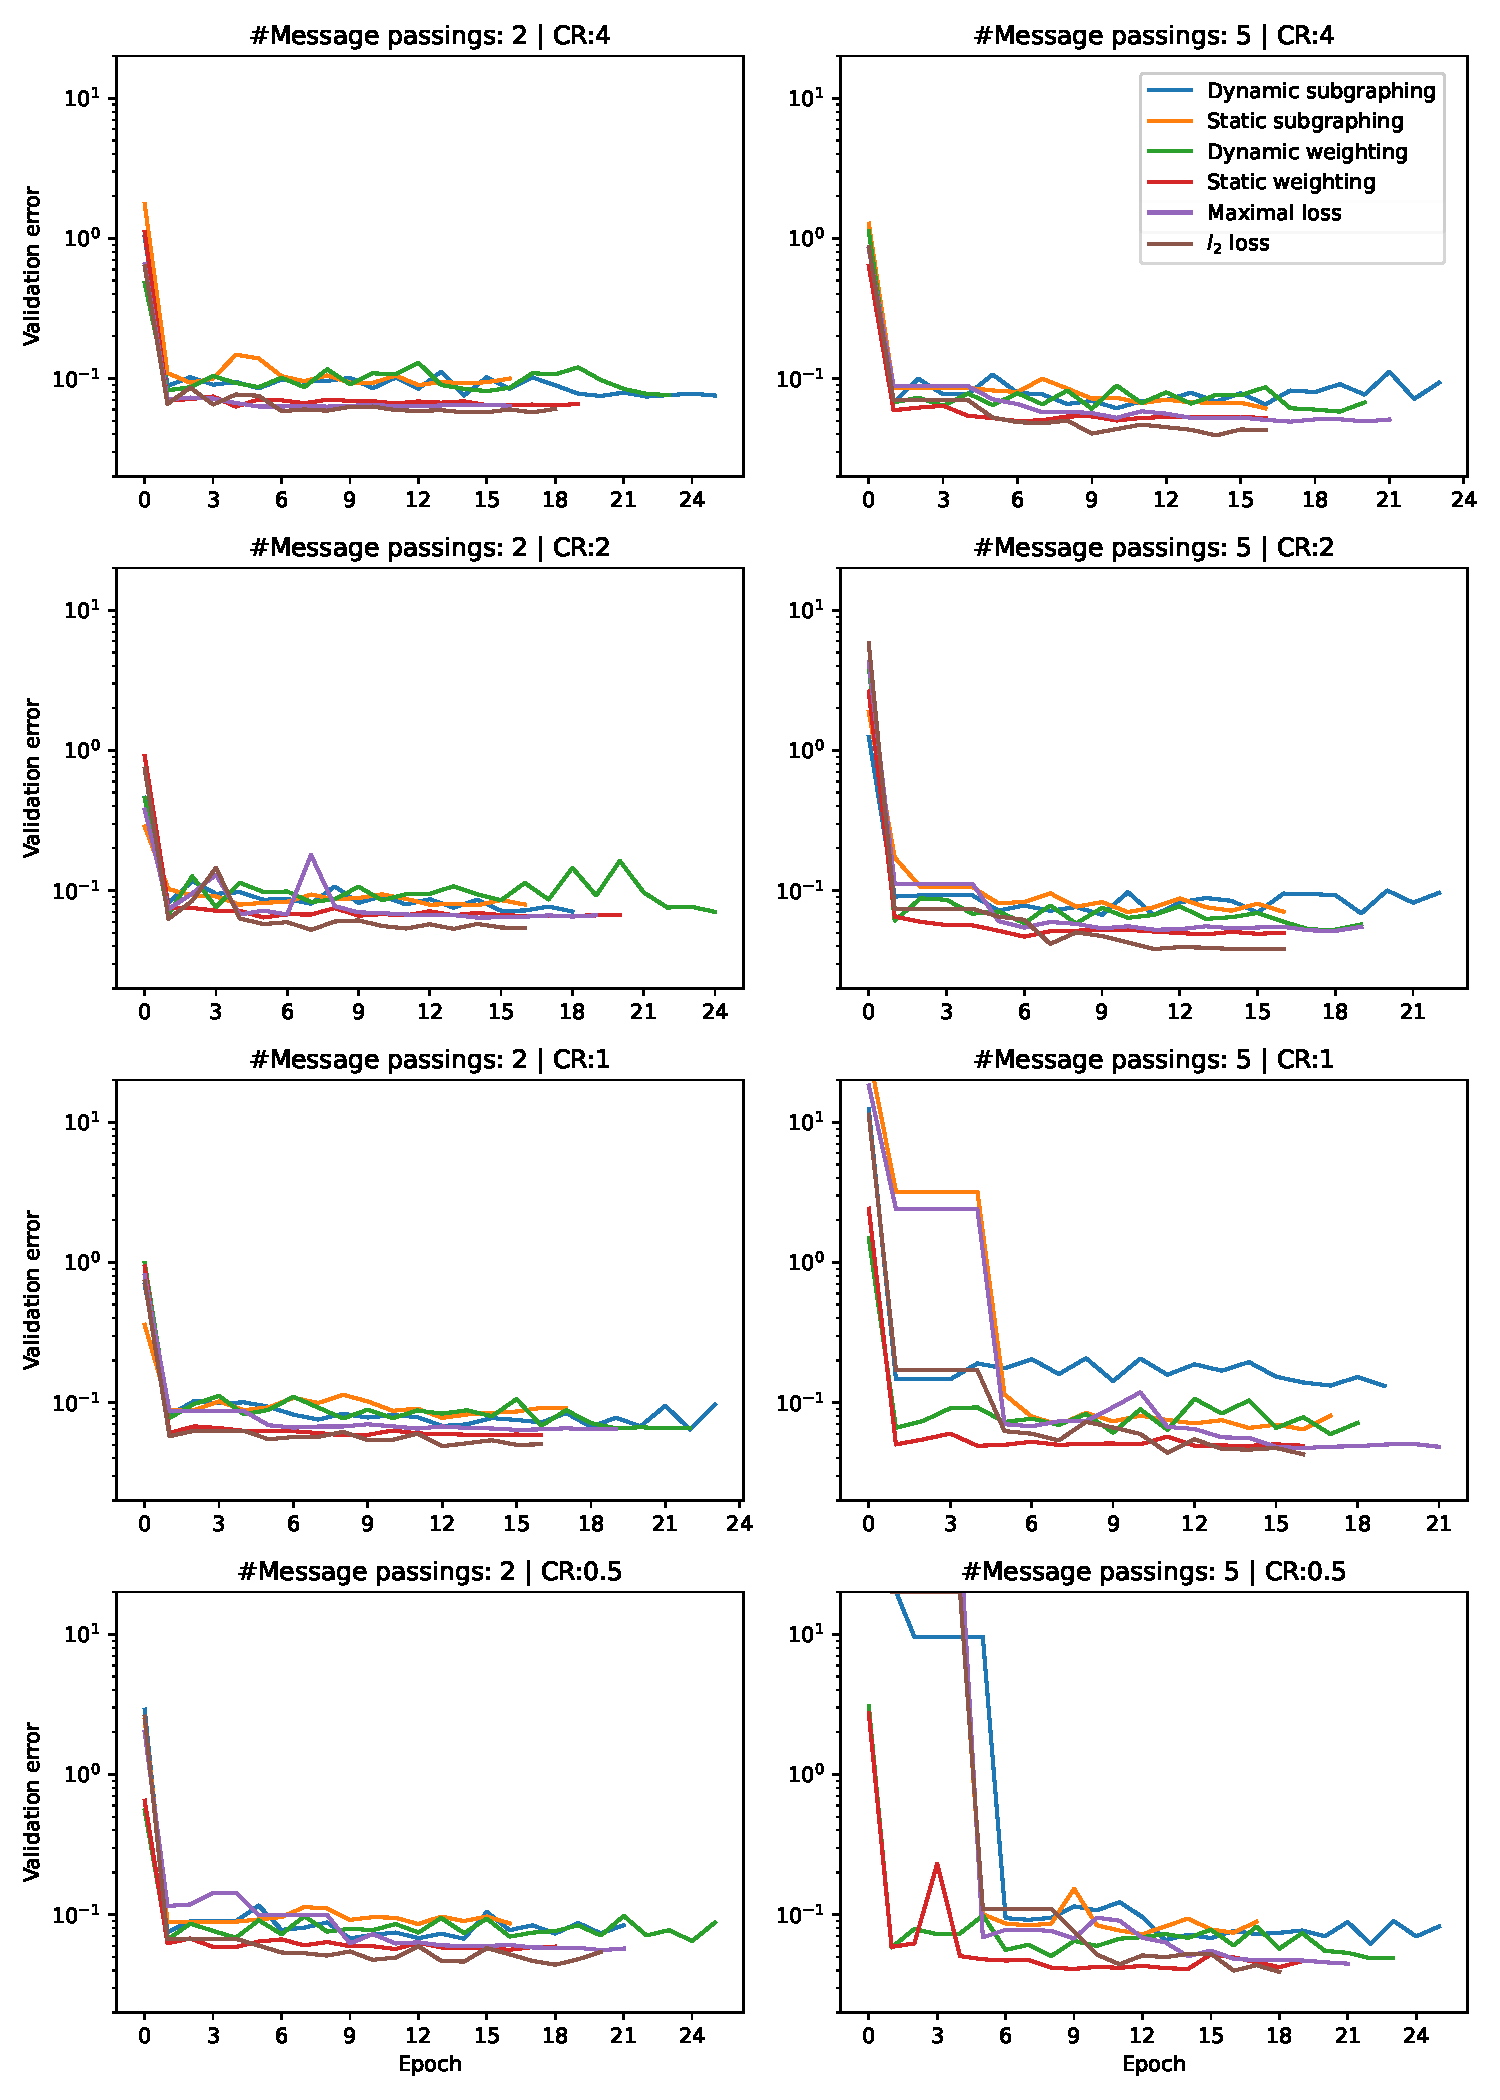
\includegraphics[width=1\linewidth,keepaspectratio]{gnn.pdf}
\caption{Comparative analysis of validation errors across training epochs for the models without AE.}\label{fig:gnn}
\end{figure}
%
\begin{figure}\centering
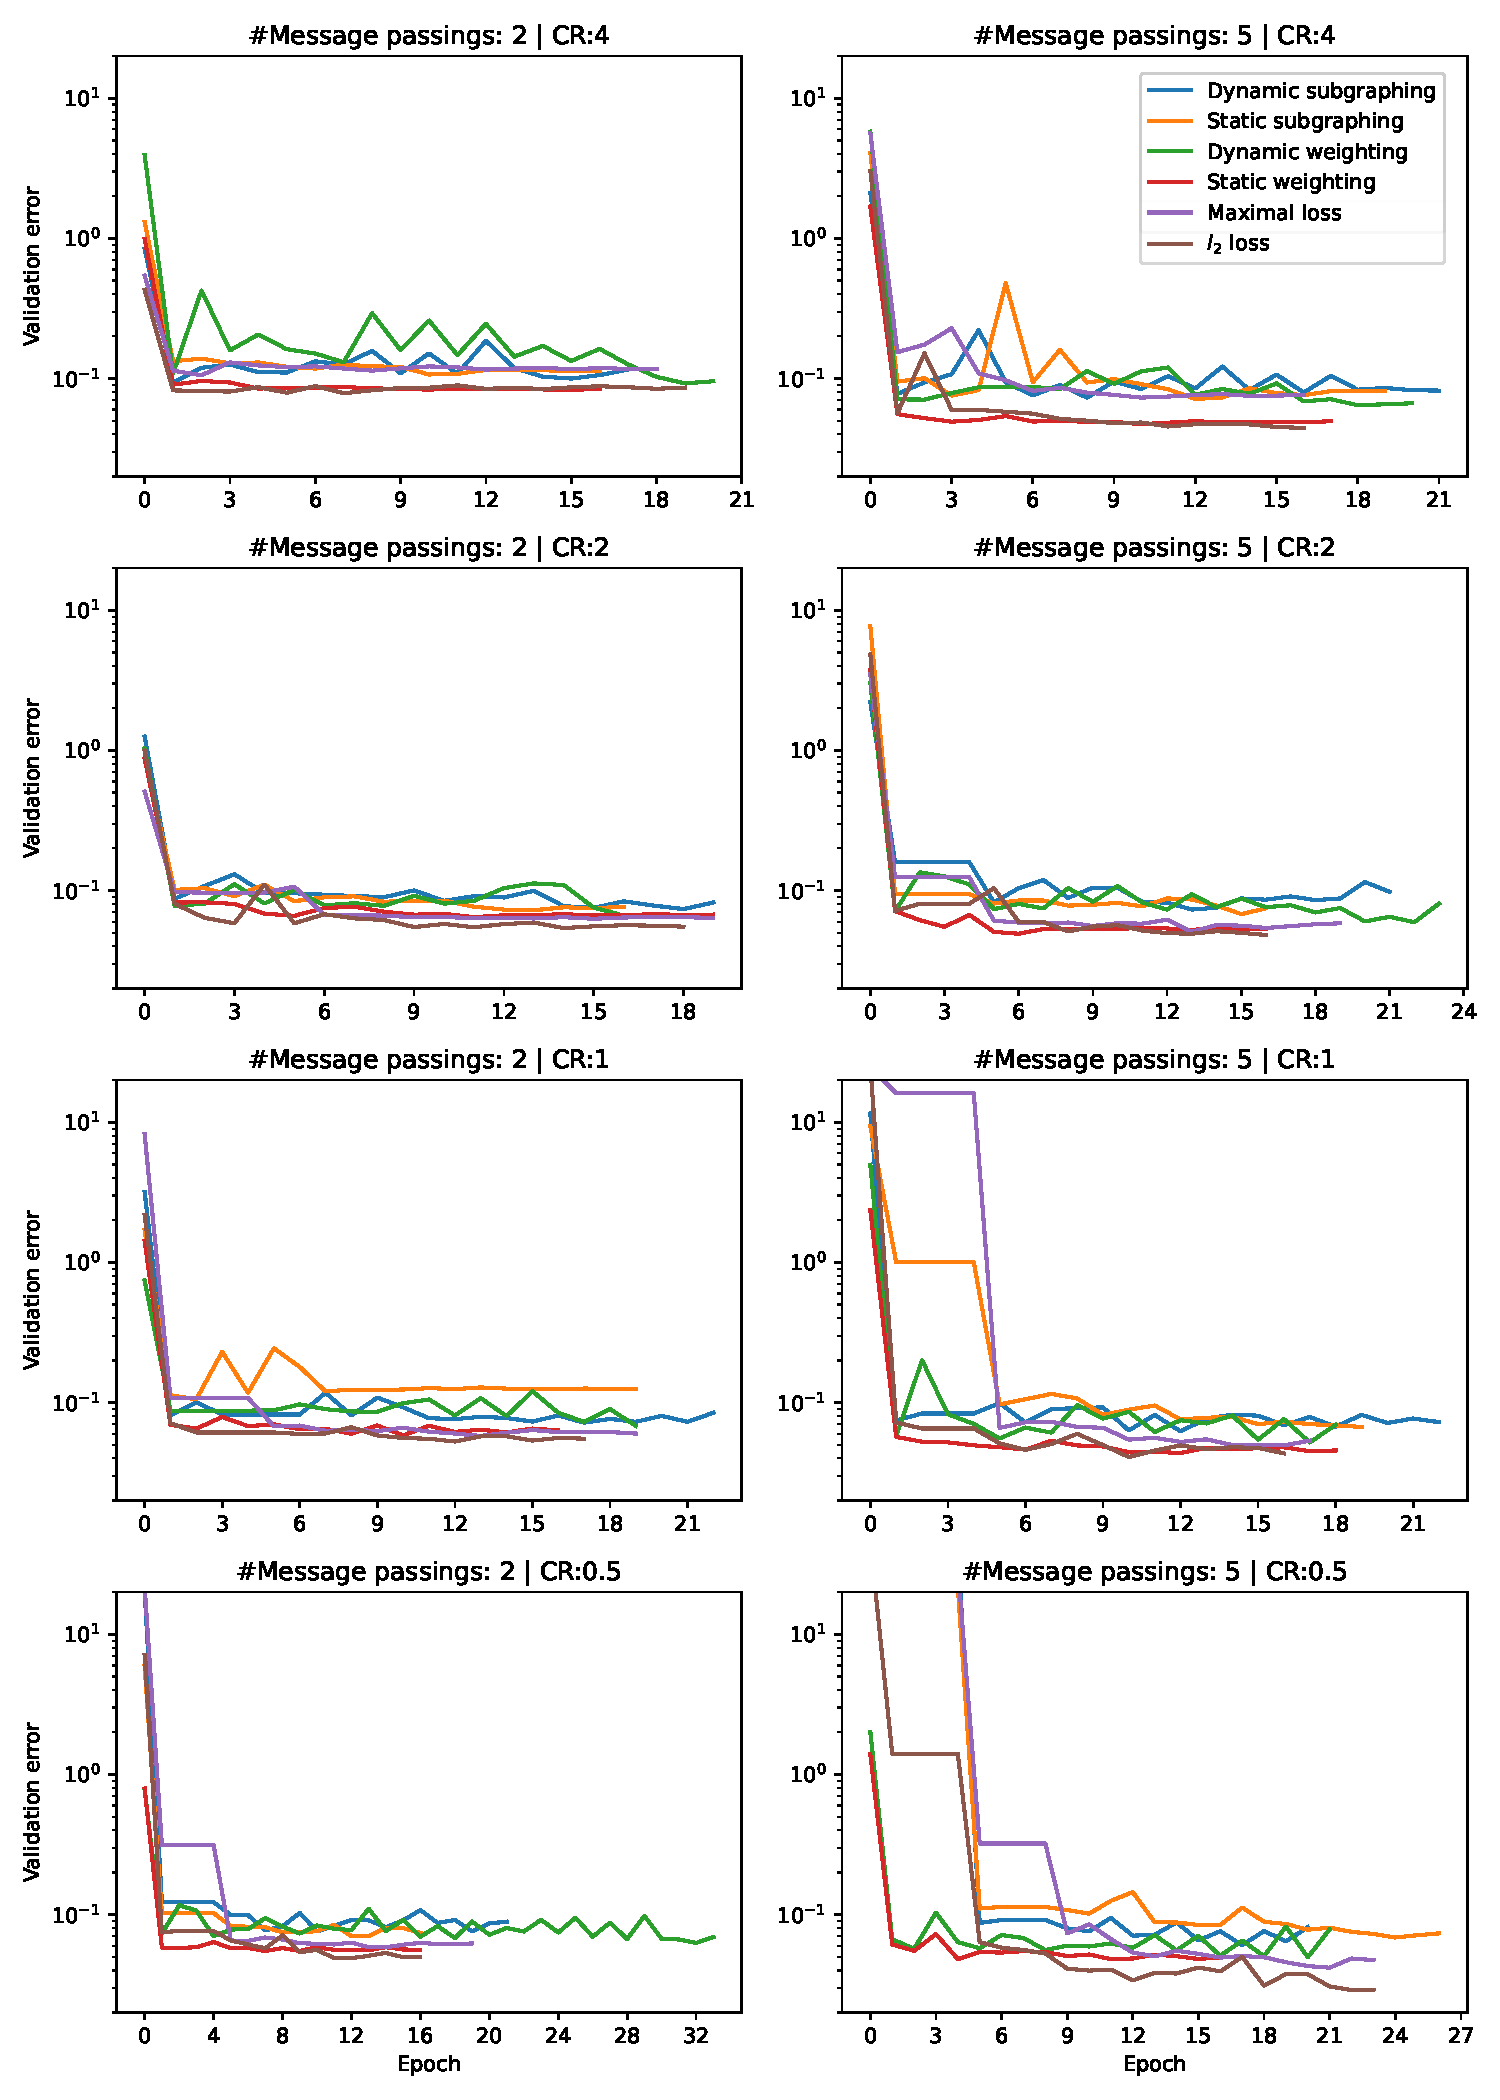
\includegraphics[width=1\linewidth,keepaspectratio]{combined.pdf}
\caption{Comparative analysis of validation errors across training epochs for the models with AE.}\label{fig:combined}
\end{figure}

\paragraph{Knee-scale simulation.} In Fig.~\ref{fig:3d_boxplot}, we present a comprehensive analysis of the out-of-distribution testing errors, as detailed in Tables~\ref{table_4_5} to \ref{table_0.5_5} in Appendix~\ref{appendix_b}. We acknowledge that the limited sample size employed in this knee-scale simulation, a constraint imposed by the infeasibility of storing an extensive array of snapshots in memory. This limitation might introduce some bias in the error metrics due to sampling variability. Despite this, a discernible pattern emerges from the aggregated data, disregarding the outliers. Remarkably, the application of more complex models, particularly with \ac{ae}, does not again manifest in substantial performance enhancements. Conversely, \ac{da} exhibits a pronounced positive impact, primarily because models devoid of augmentation lack exposure to diversified element configurations. Notably, the models implementing a weighted loss approach consistently demonstrate the most minimal error margins, coupled with a markedly lower variance.
%
\begin{figure}[t!]\centering
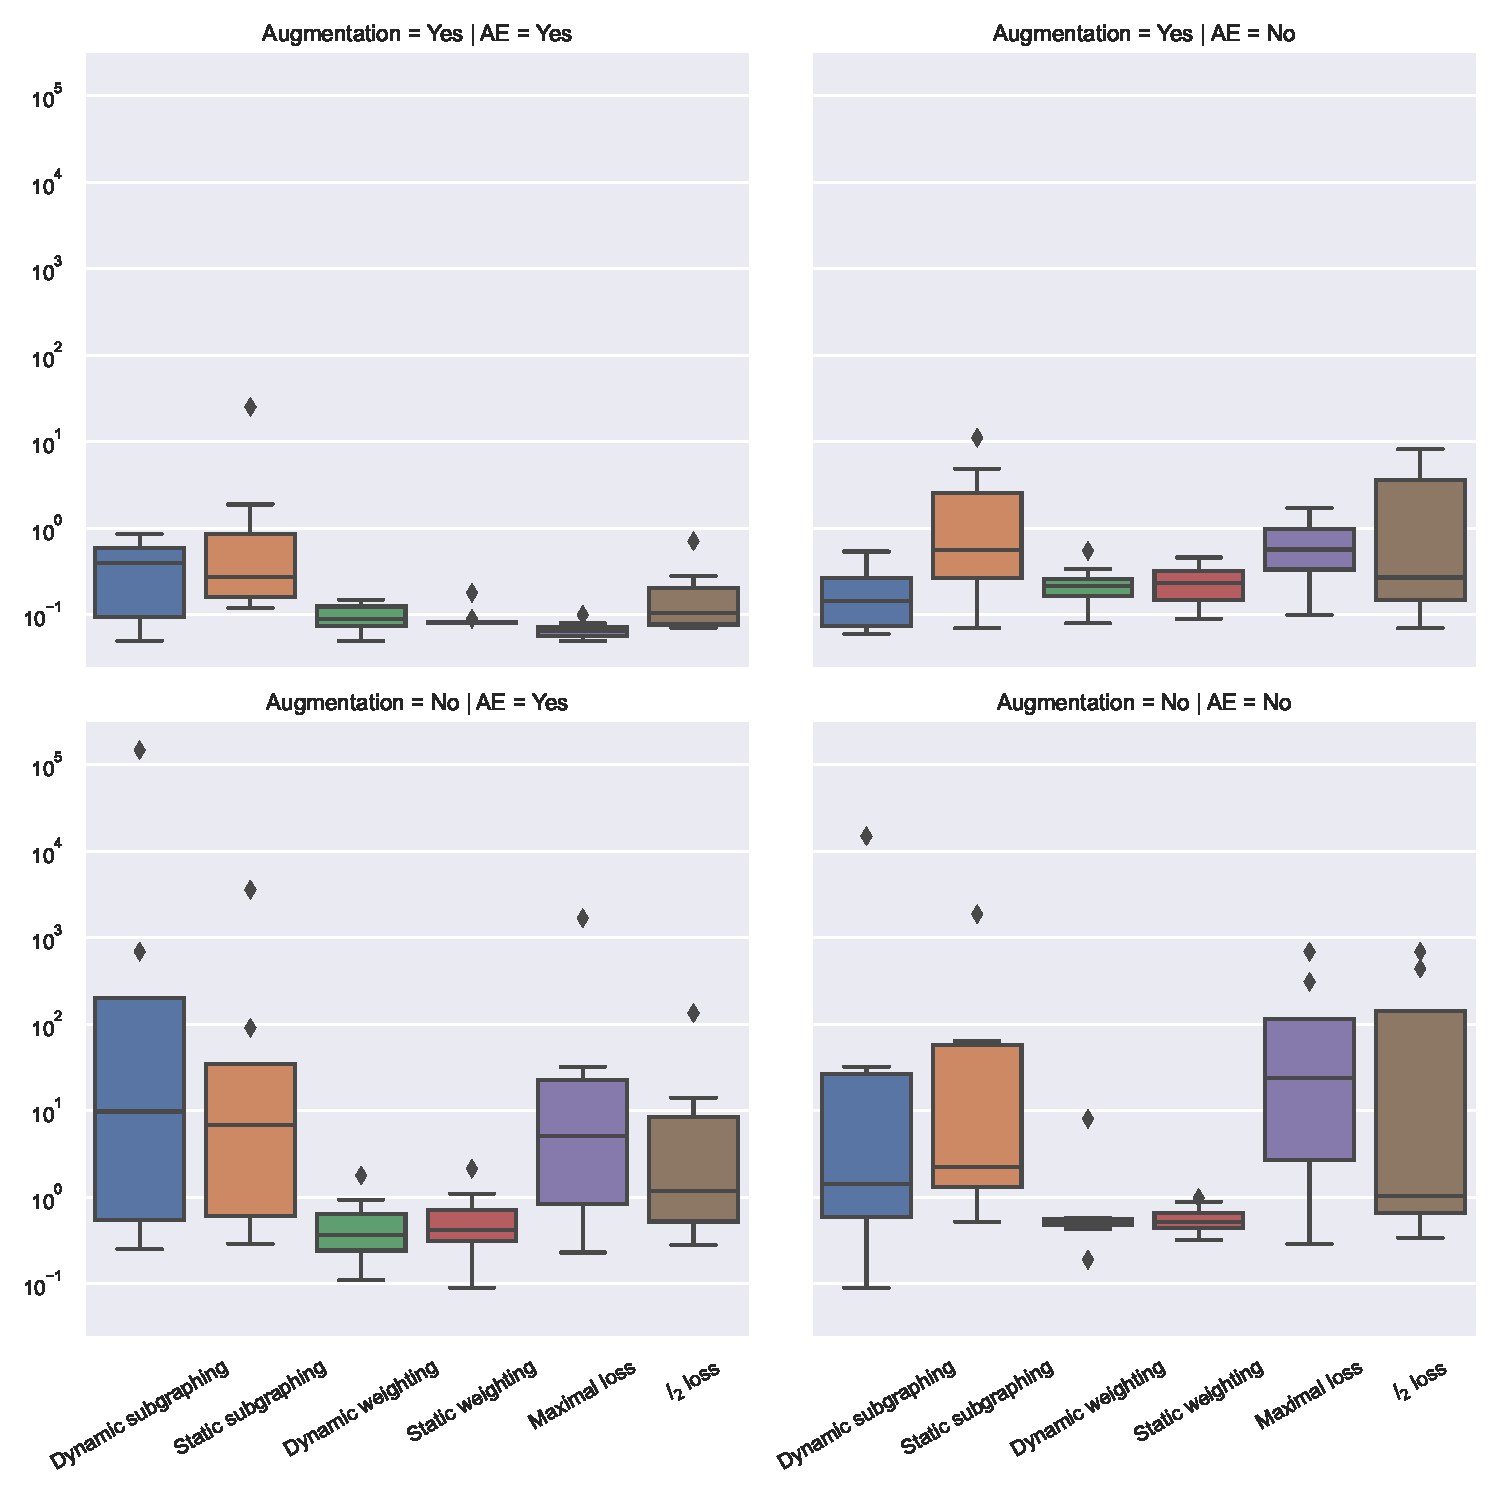
\includegraphics[width=1\linewidth,keepaspectratio]{3d_boxplot.pdf}
\caption{Averaged out-of-distribution testing errors for various models trained using different loss functions.}\label{fig:3d_boxplot}
\end{figure}

To further assess the efficacy of our novel graph-based \ac{da} technique, we examined the averaged pointwise errors, as depicted in Fig.~\ref{fig:3d_inductive}. Notably, the regular loss function yielded the highest errors, while the implementation of weighted loss functions resulted in significantly reduced errors, almost negligible in comparison. Although maximal loss may still hold value in simpler models, it demands very large training batch sizes. Interestingly, subgraph-based methods did not surpass the performance of weighting strategies, likely due to their specific tuning requirements. Dynamic versions of these methods, requiring minimal tuning, showed superior performance over their static counterparts with \ac{da}. Regardless of the approach used for addressing data imbalance, the application of our \ac{da} algorithm consistently achieved a substantial reduction in errors, further validating its effectiveness.
%
\begin{figure}\centering
\includegraphics[height=0.9\textheight,keepaspectratio]{3d_inductive.jpg}
\caption{Averaged pointwise out-of-distribution testing errors for various models trained using different loss functions. Illustrated values are from zero (shown in blue) to beyond 2 (shown in red).}\label{fig:3d_inductive}
\end{figure}

\paragraph{Other discussion.} We acknowledge two key limitations. First, the subgraph implementation might be too specific. Indeed, we updated the dynamic version at each training epoch instead of each step, a decision influenced by potential performance bottlenecks. This approach, while effective for our objectives, leaves room for future optimization in different training scenarios [\cite{xue2023}]. Second, although we used a complex multiphasic model (with pre-stressing) for the large-scale simulation, the numerical implementation and imposed boundary conditions are again very specific to avoid very demanding \ac{hf} data generation. However, this constraint aligns with the methodological nature of this work, as experiments are designed to evaluate the effectiveness of our extensions, particularly the \ac{da} approach, rather than executing diverse \ac{hf} simulations and biomechanical analyses.

To summarize, we proposed and empirically tested an extended \ac{hml} framework tailored for multiphasic surrogate modeling of knee cartilage, showcasing potentials in both few-shot learning and zero-shot generalization. This approach integrates a customized training loop and a hybrid (multi-fidelity) scheme, permitting efficient training. These models exhibited sufficient accuracy even with a minimal number of message-passing blocks and without \ac{ae}-based \ac{mor}. Additionally, we conducted a comparative analysis of various preprocessing, cost-sensitive, and resampling strategies, underscoring their critical role in addressing data imbalance and skewness that impacted training. Most importantly, the chapter also highlights how our proposed physics-based \ac{da} technique significantly improves the surrogate model's generalizability. Such advancements might also mitigate the prevalent issues of limited generalizability and efficiency in existing \ac{ml}-based surrogate models, potentially extending their applicability across broader multiscale domains.

\chapter{Conclusion}
%
This work is one of the first attempts to provide a multi-physics numerical and data-driven model of knee cartilage with implementation efficiency. At the heart of this study was the development of an efficient, generalizable, and scalable surrogate modeling framework, trained on a multiphasic model of cartilage across various scales and fidelities. Then, surrogate models were developed with the assumption of limited training data, as \ac{hf} biomechanical models might be too expensive to generate the data. By integrating state-of-the-art \ac{ml} and \ac{fe} analysis, we sought to overcome these challenges and developed four research questions in this regard.

Addressing the first research question, ``\textit{How can a complex multi-physics model of cartilage biomechanics be implemented efficiently enough to generate the required training datasets?}'', we successfully implemented a complex multi-physics model of cartilage biomechanics with a fully automated \ac{psa}, optimized for efficient subsequent \ac{hf} dataset generation. This model was designed with a focus on balancing computational efficiency with the numerical fidelity necessary to capture the heterogeneous and multiphasic nature of cartilage tissue. Besides, the key to efficiently generating the training datasets was found in the strategic simplification of our multi-physics cartilage model, used subsequently in a \ac{hml} method.

The second research question, ``\textit{How can machine learning techniques be integrated into the numerical model for efficient surrogate modeling?}'', was addressed through the development of a novel hybrid multi-fidelity learning framework. It combines the \ac{lf} (reduced-order) numerical analysis with model-agnostic supervised \ac{ml} techniques. The cornerstone of this integration was the creation of surrogate models that are trained on a limited number of \ac{hf} numerical samples. The surrogate models developed showcased a significant reduction in computational time compared to traditional numerical methods, achieving the goal of efficient surrogate modeling. This integration of \ac{ml} into our numerical model is a leap forward in the field, especially in the context of cartilage biomechanics.

In light of the third research question, ``\textit{Is the new machine learning system scalable and generalizable across different scales}'', we expanded the scope of our study to encompass multiscale simulations. The scalability and generalizability of our \ac{hml} framework were rigorously tested by employing it in both tissue-scale and knee-scale simulations. We tested the integration of an upstream \ac{ae} model, along with the application of various preprocessing and customization algorithms, to evaluate their effects on performance. Our findings suggest that the augmented \ac{hml} framework, combined with \acp{gnn}, can effectively learn from small-scale data and generalize its knowledge to larger, more complex simulations, thereby answering positively this question.

Addressing the final research question, ``\textit{What are the potential implications of the proposed methods for future research?}'', we believe that our proposed methods can significantly contribute to future development due to their non-intrusive implementation of advanced cartilage biomechanics. Our \ac{hf} pre-stressed and multi-physics cartilage model can be efficiently implemented since it is based on a combination of regular nonlinear \ac{fe} and a \ac{fpbbs}. The data-driven extensions also are based on widely adopted \ac{dl} algorithms, again with efficient execution and fast training. Additionally, as similar models are extensively developed in biomechanics, the implications of this research are far-reaching, potentially providing a new template for efficiently implementing simulations without sacrificing constitutive complexity.

Nonetheless, during our evaluation, we designed the simulations specifically to efficiently generate datasets. We recognize this as a limitation but have strived to enhance the generalizability of our results by implementing complex biomechanical models in various scenarios. However, for application-oriented studies, further research may be needed to devise the best strategies for generating the most informative training samples corresponding to each biomechanical simulation. Since sample-wise validation of the model may not be generalizable or even feasible, especially in large-scale testing where we may have zero testing samples in practice, we may resort to further available evaluation errors. However, these metrics also have their limits [\cite{barocas2023}] and therefore cannot replace rigorous \textit{in vivo} or \textit{in vitro} validation. Such tests, however, are highly time-consuming and problem-specific and thus remain for future studies.

Among possible future directions to advance our method is the integration of generative models [\cite{rezende2014,kingma2014}], to replace the preprocessing steps. This integration could accelerate preprocessing tasks and potentially eliminate the need for our custom training loops. Furthermore, applying our method to more advanced, simulation-specific analyses, especially with more complex boundary conditions [\cite{lenhart2015}], is another interesting research direction. In particular, our hybrid method has significant potential to expedite the repetitive process of cartilage analysis, e.g., [\cite{elahi2021}], particularly when incorporating osmotic pressure, as in [\cite{elahi2023}]. Also, since it has been successfully tested for zero-shot generalization, it might be applied for very interesting multiscale modeling with even non-iterative tasks at large-scale, while trained on small-scale data.

On the other hand, while \ac{ml} studies have embraced the open-source culture, e.g., [\cite{panfilov2019,desai2019,desai2021,thomas2021,panfilov2022}], numerical studies in biomechanics are rarely open-sourced, likely due to legal complexities, which complicates the future testing and advancement of our methods. Recently, a few biomechanical or numerical studies have started to democratize the field by sharing their code, e.g., [\cite{fehervary2020,maes2023,chokhandre2021}], but the scarcity of such models remains a major challenge for future progress. As a remedy, we have open-sourced most of our data, accompanied by detailed documentation.

To conclude, we summarize our main original contributions, which were empirically tested throughout this research, as follows:
%
\begin{enumerate}
    \item Development of a cartilage model, optimized for automatic generation of \ac{hf} training data, with its merits demonstrated by pre-stressing simulation to assess its impact on constitutive behavior and tissue biomechanics.
    \item Development of straightforward \ac{hml} in the context of soft tissue multi-physics, enabling multi-fidelity surrogate modeling of cartilage regardless of the \ac{ml} model employed.
    \item Extension of the hybrid model with a set of relatively efficient algorithms, particularly physics-based \ac{da}, permitting multiscale surrogate modeling, implemented by using \acp{gnn}.
\end{enumerate}
%
Furthermore, our research may transcend its initial biomechanical application, showcasing a harmonious blend of learnable AI with traditional numerical analysis, while emphasizing the balance between efficiency and complexity under limited resources.

% References
\printbibliography[title={References}, heading=bibintoc]

% Appendices
%\renewcommand{\appendixname}{Appendices}
%\appendix

\begin{appendices}
\chapter{Runtime Details}\label{appendix_1}

\begin{longtable}{lcccc}
\caption{Runtime details, on a regular \ac{cpu}, corresponding data generation of small-scale numerical samples used in Chapter~\ref{ch4}.}
\label{table:hml_2d_runtime}
\\\toprule
\textbf{2D Sample} & \multicolumn{2}{c}{\textbf{LF model}} & \multicolumn{2}{c}{\textbf{HF model}} \\\cmidrule{2-3} \cmidrule{4-5}
 & {Min} & {Sec} & {Min}  & {Sec} \\
\midrule
\endfirsthead
\multicolumn{5}{@{}l}{\ldots continued}\\\toprule
\textbf{2D Sample} & \multicolumn{2}{c}{\textbf{LF model}} & \multicolumn{2}{c}{\textbf{HF model}} \\\cmidrule{2-3} \cmidrule{4-5}
 & {Min} & {Sec} &  {Min}  & {Sec} \\
\midrule
\endhead
1   &   0 &  21 &   2 &  21 \\
2   &   0 &  21 &   2 &  21 \\
3   &   0 &  21 &   2 &  21 \\
4   &   0 &  21 &   2 &  21 \\
5   &   0 &  21 &   2 &  21 \\
6   &   0 &  21 &   2 &  21 \\
7   &   0 &  21 &   2 &  20 \\
8   &   0 &  21 &   2 &  19 \\
9   &   0 &  21 &   2 &  22 \\
10  &   0 &  21 &   2 &  21 \\
11  &   0 &  21 &   2 &  21 \\
12  &   0 &  21 &   2 &  21 \\
13  &   0 &  21 &   2 &  21 \\
14  &   0 &  21 &   2 &  21 \\
15  &   0 &  21 &   2 &  21 \\
16  &   0 &  21 &   2 &  21 \\
17  &   0 &  21 &   2 &  21 \\
18  &   0 &  21 &   2 &  22 \\
19  &   0 &  21 &   2 &  21 \\
20  &   0 &  21 &   2 &  22 \\
21  &   0 &  21 &   2 &  21 \\
22  &   0 &  21 &   2 &  22 \\
23  &   0 &  21 &   2 &  22 \\
24  &   0 &  21 &   2 &  22 \\
25  &   0 &  21 &   2 &  22 \\
26  &   0 &  21 &   2 &  21 \\
27  &   0 &  21 &   2 &  21 \\
28  &   0 &  21 &   2 &  22 \\
29  &   0 &  21 &   2 &  22 \\
30  &   0 &  21 &   2 &  22 \\
31  &   0 &  24 &   2 &  11 \\
32  &   0 &  18 &   2 &  10 \\
33  &   0 &  18 &   2 &  10 \\
34  &   0 &  18 &   2 &  10 \\
35  &   0 &  18 &   2 &  10 \\
36  &   0 &  19 &   2 &  11 \\
37  &   0 &  18 &   2 &  11 \\
38  &   0 &  18 &   1 &  51 \\
39  &   0 &  18 &   2 &  10 \\
40  &   0 &  18 &   2 &  11 \\
\bottomrule
\end{longtable}

\begin{longtable}{lcccc}
\caption{Runtime details, on a regular \ac{cpu}, corresponding data generation of large-scale numerical samples used in Chapter~\ref{ch4}.}
\label{table:hml_3d_runtime}
\\\toprule
\textbf{3D Sample} & \multicolumn{2}{c}{\textbf{LF model}} & \multicolumn{2}{c}{\textbf{HF model}} \\\cmidrule{2-3} \cmidrule{4-5}
 & {Min} & {Sec} &  {Min}  & {Sec} \\
\midrule
\endfirsthead
\multicolumn{5}{@{}l}{\ldots continued}\\\toprule
\textbf{3D Sample} & \multicolumn{2}{c}{\textbf{LF model}} & \multicolumn{2}{c}{\textbf{HF model}} \\\cmidrule{2-3} \cmidrule{4-5}
 & {Min} & {Sec} &  {Min}  & {Sec} \\
\midrule
\endhead
1   &   1 &  22 &  10 &  22 \\
2   &   1 &   5 &   7 &  31 \\
3   &   1 &   1 &   7 &  37 \\
4   &   1 &  51 &  14 &  23 \\
5   &   1 &   9 &  11 &  53 \\
6   &   1 &   7 &  11 &  40 \\
7   &   1 &  19 &   9 &  54 \\
8   &   1 &  11 &  12 &   2 \\
9   &   1 &  31 &   9 &   2 \\
10  &   1 &  23 &  12 &  19 \\
11  &   1 &   3 &   7 &  11 \\
12  &   1 &  15 &  11 &  27 \\
13  &   1 &  23 &   8 &  37 \\
14  &   1 &  53 &  14 &  22 \\
15  &   1 &  13 &   7 &  15 \\
16  &   1 &  25 &  14 &  50 \\
17  &   1 &   5 &   4 &   2 \\
18  &   1 &  17 &  11 &  40 \\
19  &   1 &   7 &   7 &  29 \\
20  &   1 &   5 &   7 &  18 \\
21  &   0 &  59 &   7 &  25 \\
22  &   2 &   3 &  20 &  48 \\
23  &   1 &  15 &  12 &  36 \\
24  &   1 &  29 &   9 &  57 \\
25  &   1 &  11 &   7 &  20 \\
26  &   1 &  21 &  12 &  14 \\
27  &   1 &  17 &   7 &  13 \\
28  &   1 &   5 &   8 &   7 \\
29  &   1 &  23 &  13 &  50 \\
30  &   1 &  11 &  12 &  58 \\
31  &   1 &   0 &   7 &  55 \\
32  &   2 &  13 &  17 &  15 \\
33  &   1 &   7 &   7 &  53 \\
34  &   1 &  25 &  15 &  43 \\
35  &   1 &   5 &   7 &  42 \\
36  &   1 &   9 &   7 &  25 \\
37  &   1 &   9 &  10 &  30 \\
38  &   1 &   3 &   4 &  18 \\
39  &   1 &  19 &  10 &   5 \\
40  &   1 &  23 &  14 &  18 \\
41  &   1 &  11 &  10 &  58 \\
42  &   1 &  17 &   7 &  55 \\
43  &   1 &  13 &  11 &  52 \\
44  &   1 &  29 &  15 &  39 \\
45  &   1 &  13 &  13 &  14 \\
46  &   1 &   7 &   4 &  36 \\
47  &   1 &  17 &  19 &  32 \\
48  &   1 &  19 &  10 &  28 \\
49  &   1 &   3 &   7 &  35 \\
50  &   1 &   7 &   4 &  14 \\
51  &   1 &  21 &  14 &   1 \\
52  &   1 &  21 &  12 &  36 \\
53  &   1 &  43 &  13 &  10 \\
54  &   1 &  23 &  15 &   5 \\
55  &   1 &   4 &   9 &   5 \\
56  &   1 &  23 &  13 &  38 \\
57  &   2 &   3 &  21 &  21 \\
58  &   1 &  21 &   9 &  39 \\
59  &   1 &  17 &  10 &  17 \\
60  &   1 &   7 &   7 &  25 \\
61  &   1 &   7 &   8 &  29 \\
62  &   1 &   3 &   8 &  48 \\
63  &   1 &  53 &  14 &  19 \\
64  &   1 &  19 &   9 &   4 \\
65  &   1 &  51 &  13 &  52 \\
66  &   1 &  43 &  15 &   7 \\
67  &   1 &  15 &  13 &  25 \\
68  &   1 &   9 &  11 &  31 \\
69  &   1 &   7 &   7 &  23 \\
70  &   1 &  33 &  13 &   3 \\
71  &   1 &  17 &  18 &  24 \\
72  &   1 &  43 &  13 &  36 \\
73  &   1 &  21 &   9 &  36 \\
74  &   1 &  15 &   9 &  18 \\
75  &   1 &   3 &   7 &  40 \\
76  &   1 &  23 &  12 &  21 \\
77  &   1 &  11 &  10 &  10 \\
78  &   1 &  19 &   9 &  50 \\
79  &   2 &   5 &  13 &   1 \\
80  &   1 &  17 &   9 &   8 \\
81  &   1 &  21 &  12 &  17 \\
82  &   1 &  39 &  14 &  36 \\
83  &   1 &   7 &  11 &  31 \\
84  &   1 &  37 &  13 &   3 \\
85  &   1 &   7 &   7 &   8 \\
86  &   1 &  23 &   9 &  42 \\
87  &   2 &  17 &  15 &  32 \\
88  &   1 &  17 &   8 &  42 \\
89  &   1 &  13 &   9 &  58 \\
90  &   1 &  19 &   8 &  34 \\
91  &   1 &   5 &   3 &  54 \\
92  &   1 &   5 &   8 &  28 \\
93  &   1 &   7 &   7 &   7 \\
94  &   1 &   9 &  10 &  37 \\
95  &   1 &  11 &   9 &  54 \\
96  &   1 &   5 &   7 &   7 \\
97  &   1 &   1 &   8 &   8 \\
98  &   2 &  11 &  15 &   8 \\
99  &   1 &   1 &   8 &   2 \\
100 &   1 &   2 &   4 &   6 \\
\bottomrule
\end{longtable}

\begin{longtable}{lcccc}
\caption{Runtime details, on a regular \ac{cpu}, corresponding data generation of small-scale numerical samples used in Chapter~\ref{ch5}.}
\label{table:smallscale_runtime}
\\\toprule
\textbf{Small-scale sample} & \multicolumn{2}{c}{\textbf{LF model}} & \multicolumn{2}{c}{\textbf{HF model}} \\\cmidrule{2-3} \cmidrule{4-5}
 & {Min} & {Sec} & {Min}  & {Sec} \\
\midrule
\endfirsthead
\multicolumn{5}{@{}l}{\ldots continued}\\\toprule
\textbf{Small-scale sample} & \multicolumn{2}{c}{\textbf{LF model}} & \multicolumn{2}{c}{\textbf{HF model}} \\\cmidrule{2-3} \cmidrule{4-5}
 & {Min} & {Sec} &  {Min}  & {Sec} \\
\midrule
\endhead

1 & 1 & 1 & 21 & 29 \\
2 & 1 & 16 & 18 & 54 \\
3 & 0 & 56 & 21 & 53 \\
4 & 0 & 48 & 19 & 54 \\
5 & 3 & 56 & 19 & 51 \\
6 & 1 & 1 & 20 & 0 \\
7 & 0 & 56 & 23 & 4 \\
8 & 1 & 36 & 18 & 7 \\
9 & 1 & 31 & 16 & 44 \\
10 & 0 & 51 & 16 & 7 \\
11 & 0 & 46 & 19 & 39 \\
12 & 0 & 52 & 21 & 13 \\
13 & 1 & 21 & 19 & 38 \\
14 & 1 & 6 & 18 & 16 \\
15 & 2 & 46 & 22 & 21 \\
16 & 1 & 21 & 19 & 19 \\
17 & 1 & 31 & 19 & 53 \\
18 & 0 & 56 & 21 & 22 \\
19 & 0 & 51 & 20 & 13 \\
20 & 0 & 46 & 23 & 6 \\
21 & 0 & 52 & 22 & 27 \\
22 & 1 & 6 & 20 & 43 \\
23 & 1 & 32 & 18 & 10 \\
24 & 1 & 21 & 19 & 0 \\
25 & 1 & 6 & 22 & 52 \\
26 & 1 & 42 & 24 & 10 \\
27 & 4 & 12 & 19 & 10 \\
28 & 1 & 22 & 20 & 45 \\
29 & 0 & 46 & 21 & 20 \\
30 & 1 & 26 & 24 & 3 \\
31 & 2 & 1 & 21 & 32 \\
32 & 1 & 12 & 21 & 45 \\
33 & 1 & 41 & 21 & 41 \\
34 & 1 & 6 & 27 & 0 \\
35 & 0 & 56 & 23 & 56 \\
36 & 0 & 46 & 21 & 34 \\
37 & 1 & 1 & 20 & 55 \\
38 & 1 & 2 & 22 & 32 \\
39 & 1 & 8 & 17 & 42 \\
40 & 0 & 56 & 24 & 11 \\
41 & 0 & 52 & 22 & 54 \\
42 & 1 & 56 & 22 & 14 \\
43 & 0 & 58 & 23 & 9 \\
44 & 0 & 46 & 21 & 35 \\
45 & 1 & 11 & 20 & 20 \\
46 & 0 & 56 & 22 & 37 \\
47 & 1 & 11 & 21 & 6 \\
48 & 1 & 21 & 21 & 27 \\
49 & 1 & 21 & 23 & 45 \\
50 & 1 & 6 & 24 & 38 \\
\bottomrule
\end{longtable}

\begin{longtable}{lcccc}
\caption{Runtime details, on a regular \ac{cpu}, corresponding data generation of small-scale numerical samples used in Chapter~\ref{ch5}.}
\label{table:largescale_runtime}
\\\toprule
\textbf{Large-scale sample} & \multicolumn{2}{c}{\textbf{LF model}} & \multicolumn{2}{c}{\textbf{HF model}} \\\cmidrule{2-3} \cmidrule{4-5}
 & {Min} & {Sec} & {Min}  & {Sec} \\
\midrule
\endfirsthead
\multicolumn{5}{@{}l}{\ldots continued}\\\toprule
\textbf{Large-scale sample} & \multicolumn{2}{c}{\textbf{LF model}} & \multicolumn{2}{c}{\textbf{HF model}} \\\cmidrule{2-3} \cmidrule{4-5}
 & {Min} & {Sec} &  {Min}  & {Sec} \\
\midrule
\endhead
1 & 3 & 0 & 120 & 55 \\
2 & 3 & 2 & 110 & 59 \\
3 & 3 & 28 & 114 & 38 \\
4 & 2 & 54 & 114 & 4 \\
5 & 3 & 14 & 120 & 23 \\
6 & 2 & 42 & 128 & 48 \\
\bottomrule
\end{longtable}

\chapter{Supplemental Results}\label{appendix_b}

\begin{table}[H]
\centering
\caption{In-distribution MSE of the small-scale model used in Chapter~\ref{ch5} with message passings: 2.}
\label{table_in_distribution_2}
\begin{tabular}{lcccccccc}
\toprule
 & \multicolumn{2}{r}{\textbf{CR: 4}} & \multicolumn{2}{r}{\textbf{CR 2}} & \multicolumn{2}{r}{\textbf{CR: 1}} & \multicolumn{2}{r}{\textbf{CR: 0.5}} \\
 \cmidrule{2-9}
\textbf{Model type} / with AE & No & Yes & No & Yes & No & Yes & No & Yes \\
\midrule
\textbf{Dynamic subgraphing} & 0.08 & 0.13 & 0.11 & 0.08 & 0.07 & 0.07 & 0.07 & 0.08 \\
\textbf{Static subgraphing} & 0.15 & 0.17 & 0.09 & 0.25 & 0.10 & 0.15 & 0.10 & 0.99 \\
\textbf{Dynamic weighting} & 0.09 & 0.27 & 0.07 & 0.19 & 0.08 & 0.40 & 0.07 & 0.53 \\
\textbf{Static weighting} & 0.08 & 0.21 & 0.06 & 0.31 & 0.07 & 0.41 & 0.07 & 0.34 \\
\textbf{Maximal loss} & 0.08 & 0.17 & 0.07 & 1.10 & 0.08 & 0.76 & 0.08 & 1.44 \\
\textbf{$\boldsymbol{l_2}$ loss} & 0.07 & 0.13 & 0.08 & 0.20 & 0.08 & 0.18 & 0.05 & 0.34 \\
\bottomrule
\end{tabular}
\end{table}

\begin{table}[H]
\centering
\caption{In-distribution MSE of the small-scale model used in Chapter~\ref{ch5} with message passings: 5.}
\label{table_in_distribution_5}
\begin{tabular}{lcccccccc}
\toprule
 & \multicolumn{2}{r}{\textbf{CR: 4}} & \multicolumn{2}{r}{\textbf{CR 2}} & \multicolumn{2}{r}{\textbf{CR: 1}} & \multicolumn{2}{r}{\textbf{CR: 0.5}} \\
 \cmidrule{2-9}
\textbf{Model type} / with AE & No & Yes & No & Yes & No & Yes & No & Yes \\
\midrule
\textbf{Dynamic subgraphing} & 0.06 & 0.10 & 0.08 & 0.09 & 0.17 & 0.06 & 0.10 & 0.07 \\
\textbf{Static subgraphing} & 0.10 & 0.41 & 0.10 & 0.30 & 0.09 & 0.28 & 0.10 & 1.11 \\
\textbf{Dynamic weighting} & 0.09 & 0.26 & 0.07 & 0.30 & 0.07 & 0.22 & 0.08 & 0.23 \\
\textbf{Static weighting} & 0.08 & 0.20 & 0.08 & 0.32 & 0.08 & 0.16 & 0.07 & 0.19 \\
\textbf{Maximal loss} & 0.06 & 1.80 & 0.06 & 0.33 & 0.07 & 7.48 & 0.07 & 1.10 \\
\textbf{$\boldsymbol{l_2}$ loss} & 0.06 & 0.36 & 0.09 & 0.16 & 0.08 & 26.07 & 0.07 & 0.19 \\
\bottomrule
\end{tabular}
\end{table}

\begin{table}
\centering
\caption{Out-of-distribution MSE of the full model used in Chapter~\ref{ch5} with compression ratio 4 and number of message passings 2.}
\label{table_4_2}
\begin{tabular}{lcccc}
\toprule
 & \multicolumn{2}{c}{\textbf{With augmentation}} & \multicolumn{2}{c}{\textbf{Without augmentation}} \\
 \cmidrule{2-3} \cmidrule{4-5}
\textbf{Model type} & With AE & Without AE & With AE & Without AE \\
\midrule
\textbf{Dynamic subgraphing} & 0.13 & 0.10 & 0.45 & 0.16 \\
\textbf{Static subgraphing} & 0.47 & 0.16 & 1.26 & 0.94 \\
\textbf{Dynamic weighting} & 0.09 & 0.19 & 0.43 & 14.83 \\
\textbf{Static weighting} & 0.12 & 0.67 & 0.55 & 0.99 \\
\textbf{Maximal loss} & 0.09 & 0.16 & 0.51 & 19.73 \\
\textbf{$\boldsymbol{l_2}$ loss} & 0.13 & 0.11 & 1.08 & 1.52 \\
\bottomrule
\end{tabular}
\end{table}

\begin{table}
\centering
\caption{Out-of-distribution MSE of the full model used in Chapter~\ref{ch5} with compression ratio 4 and number of message passings 5.}
\label{table_4_5}
\begin{tabular}{lcccc}
\toprule
 & \multicolumn{2}{c}{\textbf{With augmentation}} & \multicolumn{2}{c}{\textbf{Without augmentation}} \\
 \cmidrule{2-3} \cmidrule{4-5}
\textbf{Model type} & With AE & Without AE & With AE & Without AE \\
\midrule
\textbf{Dynamic subgraphing} & 1.28 & 0.15 & 7.42 & 2.52 \\
\textbf{Static subgraphing} & 0.17 & 0.59 & 18.65 & 2.68 \\
\textbf{Dynamic weighting} & 0.21 & 0.30 & 0.22 & 0.96 \\
\textbf{Static weighting} & 0.11 & 0.24 & 0.16 & 1.94 \\
\textbf{Maximal loss} & 0.11 & 2.35 & 0.47 & 0.78 \\
\textbf{$\boldsymbol{l_2}$ loss} & 0.11 & 0.43 & 12.06 & 1.15 \\
\bottomrule
\end{tabular}
\end{table}

\begin{table}
\centering
\caption{Out-of-distribution MSE of the full model used in Chapter~\ref{ch5} with compression ratio 2 and number of message passings 2.}
\label{table_2_2}
\begin{tabular}{lcccc}
\toprule
 & \multicolumn{2}{c}{\textbf{With augmentation}} & \multicolumn{2}{c}{\textbf{Without augmentation}} \\
 \cmidrule{2-3} \cmidrule{4-5}
\textbf{Model type} & With AE & Without AE & With AE & Without AE \\
\midrule
\textbf{Dynamic subgraphing} & 0.84 & 0.09 & 0.62 & 1.22 \\
\textbf{Static subgraphing} & 0.25 & 0.53 & 0.71 & 4.61 \\
\textbf{Dynamic weighting} & 0.15 & 0.37 & 0.40 & 0.80 \\
\textbf{Static weighting} & 0.13 & 0.50 & 2.05 & 0.72 \\
\textbf{Maximal loss} & 0.09 & 0.79 & 1.87 & 0.52 \\
\textbf{$\boldsymbol{l_2}$ loss} & 0.11 & 0.24 & 0.55 & 2.32 \\
\bottomrule
\end{tabular}
\end{table}

\begin{table}
\centering
\caption{Out-of-distribution MSE of the full model used in Chapter~\ref{ch5} with compression ratio 2 and number of message passings 5.}
\label{table_2_5}
\begin{tabular}{lcccc}
\toprule
 & \multicolumn{2}{c}{\textbf{With augmentation}} & \multicolumn{2}{c}{\textbf{Without augmentation}} \\
 \cmidrule{2-3} \cmidrule{4-5}
\textbf{Model type} & With AE & Without AE & With AE & Without AE \\
\midrule
\textbf{Dynamic subgraphing} & 0.09 & 0.14 & 66.11 & 56.07 \\
\textbf{Static subgraphing} & 2.83 & 2.62 & 163.23 & 100.30 \\
\textbf{Dynamic weighting} & 0.10 & 0.34 & 1.69 & 0.89 \\
\textbf{Static weighting} & 0.25 & 0.28 & 0.99 & 0.51 \\
\textbf{Maximal loss} & 0.10 & 0.20 & 3018.96 & 1279.40 \\
\textbf{$\boldsymbol{l_2}$ loss} & 0.39 & 4.29 & 26.25 & 1299.88 \\
\bottomrule
\end{tabular}
\end{table}

\begin{table}
\centering
\caption{Out-of-distribution MSE of the full model used in Chapter~\ref{ch5} with compression ratio 1 and number of message passings 2.}
\label{table_1_2}
\begin{tabular}{lcccc}
\toprule
 & \multicolumn{2}{c}{\textbf{With augmentation}} & \multicolumn{2}{c}{\textbf{Without augmentation}} \\
 \cmidrule{2-3} \cmidrule{4-5}
\textbf{Model type} & With AE & Without AE & With AE & Without AE \\
\midrule
\textbf{Dynamic subgraphing} & 0.14 & 0.33 & 0.97 & 0.65 \\
\textbf{Static subgraphing} & 0.33 & 0.08 & 0.44 & 1.80 \\
\textbf{Dynamic weighting} & 0.13 & 0.46 & 0.88 & 0.86 \\
\textbf{Static weighting} & 0.12 & 0.47 & 0.59 & 0.99 \\
\textbf{Maximal loss} & 0.13 & 0.90 & 6.06 & 68.72 \\
\textbf{$\boldsymbol{l_2}$ loss} & 0.09 & 0.19 & 0.44 & 0.53 \\
\bottomrule
\end{tabular}
\end{table}

\begin{table}
\centering
\caption{Out-of-distribution MSE of the full model used in Chapter~\ref{ch5} with compression ratio 1 and number of message passings 5.}
\label{table_1_5}
\begin{tabular}{lcccc}
\toprule
 & \multicolumn{2}{c}{\textbf{With augmentation}} & \multicolumn{2}{c}{\textbf{Without augmentation}} \\
 \cmidrule{2-3} \cmidrule{4-5}
\textbf{Model type} & With AE & Without AE & With AE & Without AE \\
\midrule
\textbf{Dynamic subgraphing} & 0.78 & 0.72 & 1159.24 & 25001.22 \\
\textbf{Static subgraphing} & 37.67 & 15.85 & 5983.59 & 3685.13 \\
\textbf{Dynamic weighting} & 0.17 & 0.20 & 0.41 & 0.84 \\
\textbf{Static weighting} & 0.11 & 0.17 & 0.76 & 0.61 \\
\textbf{Maximal loss} & 0.12 & 0.82 & 12.27 & 554.70 \\
\textbf{$\boldsymbol{l_2}$ loss} & 0.89 & 15.37 & 2.90 & 792.63 \\
\bottomrule
\end{tabular}
\end{table}

\begin{table}
\centering
\caption{Out-of-distribution MSE of the full model used in Chapter~\ref{ch5} with compression ratio 0.5 and number of message passings 2.}
\label{table_0.5_2}
\begin{tabular}{lcccc}
\toprule
 & \multicolumn{2}{c}{\textbf{With augmentation}} & \multicolumn{2}{c}{\textbf{Without augmentation}} \\
 \cmidrule{2-3} \cmidrule{4-5}
\textbf{Model type} & With AE & Without AE & With AE & Without AE \\
\midrule
\textbf{Dynamic subgraphing} & 0.58 & 0.77 & 29.05 & 2.83 \\
\textbf{Static subgraphing} & 0.18 & 0.85 & 6.17 & 3.51 \\
\textbf{Dynamic weighting} & 0.10 & 0.68 & 0.68 & 0.82 \\
\textbf{Static weighting} & 0.11 & 0.36 & 0.48 & 0.78 \\
\textbf{Maximal loss} & 0.07 & 1.14 & 35.30 & 5.81 \\
\textbf{$\boldsymbol{l_2}$ loss} & 0.16 & 7.86 & 1.05 & 1.05 \\
\bottomrule
\end{tabular}
\end{table}

\begin{table}
\centering
\caption{Out-of-distribution MSE of the full model used in Chapter~\ref{ch5} with compression ratio 0.5 and number of message passings 5.}
\label{table_0.5_5}
\begin{tabular}{lcccc}
\toprule
 & \multicolumn{2}{c}{\textbf{With augmentation}} & \multicolumn{2}{c}{\textbf{Without augmentation}} \\
 \cmidrule{2-3} \cmidrule{4-5}
\textbf{Model type} & With AE & Without AE & With AE & Without AE \\
\midrule
\textbf{Dynamic subgraphing} & 0.58 & 0.25 & 276541.50 & 46.19 \\
\textbf{Static subgraphing} & 0.75 & 6.94 & 29.73 & 118.65 \\
\textbf{Dynamic weighting} & 0.17 & 0.27 & 3.32 & 0.37 \\
\textbf{Static weighting} & 0.13 & 0.18 & 4.06 & 1.72 \\
\textbf{Maximal loss} & 0.08 & 1.92 & 60.22 & 94.65 \\
\textbf{$\boldsymbol{l_2}$ loss} & 0.25 & 0.32 & 250.52 & 76.40 \\
\bottomrule
\end{tabular}
\end{table}

\end{appendices}

\documentclass[12pt,a4paper]{report}
\usepackage[utf8]{inputenc}
\usepackage{setspace}
\onehalfspacing % Adjusted line spacing
\usepackage[hidelinks]{hyperref}
\hypersetup{
    colorlinks=true,
    linkcolor=blue,
    citecolor=blue,
    urlcolor=blue,
}
\usepackage{geometry}
% acronyms
\usepackage[nolist,nohyperlinks]{acronym}
\acrodef{2d}[2D]{two-dimensional}
\acrodef{gpu}[GPU]{graphics processing unit}
\acrodef{ai}[AI]{artificial intelligence}
\acrodef{3d}[3D]{three-dimensional}
\acrodef{ac}[AC]{articular cartilage}
\acrodef{ae}[AE]{autoencoder}
\acrodef{cpu}[CPU]{central processing unit}
\acrodef{cr}[CR]{compression ratio}
\acrodef{da}[DA]{data augmentation}
\acrodef{dl}[DL]{deep learning}
\acrodef{dz}[DZ]{deep zone}
\acrodef{ml}[ML]{machine learning}
\acrodef{mo}[MO]{material optimization}
\acrodef{mor}[MOR]{model order reduction}
\acrodef{mse}[MSE]{mean squared error}
\acrodef{mz}[MZ]{middle zone}
\acrodef{fe}[FE]{finite element}
\acrodef{ffnn}[FFNN]{feed-forward neural network}
\acrodef{fpbbs}[FPBBS]{fixed-point-based backward scheme}
\acrodef{gnn}[GNN]{graph neural network}
\acrodef{hf}[HF]{high-fidelity}
\acrodef{rom}[ROM]{reduced-order modeling}
\acrodef{hml}[HML]{hybrid \ac{ml}}
\acrodef{lf}[LF]{low-fidelity}
\acrodef{pmse}[PMSE]{pointwise \ac{mse}}
\acrodef{psa}[PSA]{pre-stressing algorithm}
\acrodef{sz}[SZ]{superficial zone}
%

% Adjust the page dimensions
\geometry{top=2.5cm,bottom=2.5cm,left=2.5cm,right=2.5cm}
\pagestyle{empty}
\usepackage{enumitem}

\begin{document}

\begin{center}
   {\Large
    \vspace{0.5em} % Adjust space before the title
    \textbf{Hybrid Machine Learning and Numerical Analysis of Cartilage Biomechanics}%
    \par % Ends the paragraph here, which is important for the line break
   }
   \vspace{1.5em} % Adjust space after the title
   By Seyed Shayan Sajjadinia
\end{center}

\paragraph{Abstract.} \Ac{ac}, a soft tissue essential for pain-free movement, faces significant biomechanical stress, making it a prime subject for research, especially via non-invasive computer simulations. These simulations often employ time-consuming numerical methods like \ac{fe} analysis. \Ac{ai}, offering a faster alternative, utilizes \ac{ml} as a surrogate model, which replicates numerical analysis using samples of numerical data. However, this approach can be inefficient due to the requirement for extensive training and large datasets. This study introduces an efficient, advanced biomechanical model using multi-physics modeling and a novel \ac{psa}. It generates a limited number of training samples across various fidelities and scales. Subsequently, we propose efficient, multi-fidelity, generalizable surrogate models with innovative preprocessing and training algorithms. These models integrate non-intrusive reduced-order modeling of the multi-physics equation with upstream \ac{ml}. Our empirical results underline the importance of pre-stressing in multiphasic modeling, which entails time-intensive numerical execution. This highlights the utility of efficient surrogate modeling. The surrogate models are then empirically tested, showing a substantial reduction in computational time. Moreover, the scalability and generalizability of the \ac{hml} framework are rigorously evaluated through multiscale simulations. The findings demonstrate the significant impact of our proposed physics-constrained \ac{da} and \ac{gnn} implementation. Therefore, while this study potentially advances the field with the developed \ac{psa} algorithm, it also presents an effective approach to address computational challenges and data scarcity in \ac{ml}-based surrogate modeling of cartilage biomechanics. Besides, this research, though tailored to specific cartilage modeling, potentially paves the way for broader applications of our synergistic methodology through its open-source availability.


\pagebreak

\begin{center}
   \textbf{\Large List of Activities during PhD Studies}\\
\end{center}

\begin{enumerate}[leftmargin=*]
    \item Performing a PhD project and disseminating results, as detailed at the beginning of the PhD dissertation and summarized as follows:
    \begin{itemize}
        \item Publication of two peer-reviewed papers at top journals (ranked Q1 when published), with another manuscript currently under review.
        \item Publication of one peer-reviewed conference proceedings paper, along with another recently accepted conference paper.
        \item Presentation of four conference abstracts (half presented through posters and the other half through oral presentations).
        \item Contributed an invited chapter to a forth-coming Wiley book.
        \item Open-sourcing most of the research code, such as the Python scripts and Fortran subroutines, with detailed documentation.
    \end{itemize}
    \item Participation in educational training programs, including:
    \begin{itemize}
        \item Two PhD courses focusing on research methods.
        \item Two technical courses in machine learning.
        \item One course on academic writing in English.
        \item Three summer schools: one in biomechanics (including a short oral presentation), and two others in \textit{in silico} medicine and advanced data science.
        \item One seminar on knowledge representation (including a short oral presentation).
    \end{itemize}
    \item Involvement in volunteer activities such as:
    \begin{itemize}
        \item Serving as a teaching assistant for an undergraduate mathematics course.
        \item Peer reviewing for top journals, as listed at \href{https://orcid.org/0000-0002-0789-6394}{orcid.org/0000-0002-0789-6394}.
    \end{itemize}
    \item Other activities:
    \begin{itemize}
        \item Reporting a mandatory and extensive literature review.
        \item Networking and collaborating with an international team of researchers.
        \item Attending yearly exams and presentations for project readers.
        \item Periodically presenting written and verbal updates of work to the supervisor.
        \item Self-learning research-related topics, such as graph neural networks.
        \item Attending general C1 English and A1-B1 Italian courses.
        \item Presenting a poster at a faculty evaluation meeting (invited by the faculty as one of the top five PhD students).
    \end{itemize}
\end{enumerate}

\end{document}


\end{document}
